
% Default to the notebook output style



% Tell the templating engine what output template we want to use.

% Default to the notebook output style


% Inherit from the specified cell style.




    
\documentclass{article}

    
    
    \usepackage{graphicx} % Used to insert images
    \usepackage{adjustbox} % Used to constrain images to a maximum size 
    \usepackage{color} % Allow colors to be defined
    \usepackage{enumerate} % Needed for markdown enumerations to work
    \usepackage{geometry} % Used to adjust the document margins
    \usepackage{amsmath} % Equations
    \usepackage{amssymb} % Equations
    \usepackage{eurosym} % defines \euro
    \usepackage[mathletters]{ucs} % Extended unicode (utf-8) support
    \usepackage[utf8x]{inputenc} % Allow utf-8 characters in the tex document
    \usepackage{fancyvrb} % verbatim replacement that allows latex
    \usepackage{grffile} % extends the file name processing of package graphics 
                         % to support a larger range 
    % The hyperref package gives us a pdf with properly built
    % internal navigation ('pdf bookmarks' for the table of contents,
    % internal cross-reference links, web links for URLs, etc.)
    \usepackage{hyperref}
    \usepackage{longtable} % longtable support required by pandoc >1.10
    \usepackage{booktabs}  % table support for pandoc > 1.12.2
    

    
    
    \definecolor{orange}{cmyk}{0,0.4,0.8,0.2}
    \definecolor{darkorange}{rgb}{.71,0.21,0.01}
    \definecolor{darkgreen}{rgb}{.12,.54,.11}
    \definecolor{myteal}{rgb}{.26, .44, .56}
    \definecolor{gray}{gray}{0.45}
    \definecolor{lightgray}{gray}{.95}
    \definecolor{mediumgray}{gray}{.8}
    \definecolor{inputbackground}{rgb}{.95, .95, .85}
    \definecolor{outputbackground}{rgb}{.95, .95, .95}
    \definecolor{traceback}{rgb}{1, .95, .95}
    % ansi colors
    \definecolor{red}{rgb}{.6,0,0}
    \definecolor{green}{rgb}{0,.65,0}
    \definecolor{brown}{rgb}{0.6,0.6,0}
    \definecolor{blue}{rgb}{0,.145,.698}
    \definecolor{purple}{rgb}{.698,.145,.698}
    \definecolor{cyan}{rgb}{0,.698,.698}
    \definecolor{lightgray}{gray}{0.5}
    
    % bright ansi colors
    \definecolor{darkgray}{gray}{0.25}
    \definecolor{lightred}{rgb}{1.0,0.39,0.28}
    \definecolor{lightgreen}{rgb}{0.48,0.99,0.0}
    \definecolor{lightblue}{rgb}{0.53,0.81,0.92}
    \definecolor{lightpurple}{rgb}{0.87,0.63,0.87}
    \definecolor{lightcyan}{rgb}{0.5,1.0,0.83}
    
    % commands and environments needed by pandoc snippets
    % extracted from the output of `pandoc -s`
    \providecommand{\tightlist}{%
      \setlength{\itemsep}{0pt}\setlength{\parskip}{0pt}}
    \DefineVerbatimEnvironment{Highlighting}{Verbatim}{commandchars=\\\{\}}
    % Add ',fontsize=\small' for more characters per line
    \newenvironment{Shaded}{}{}
    \newcommand{\KeywordTok}[1]{\textcolor[rgb]{0.00,0.44,0.13}{\textbf{{#1}}}}
    \newcommand{\DataTypeTok}[1]{\textcolor[rgb]{0.56,0.13,0.00}{{#1}}}
    \newcommand{\DecValTok}[1]{\textcolor[rgb]{0.25,0.63,0.44}{{#1}}}
    \newcommand{\BaseNTok}[1]{\textcolor[rgb]{0.25,0.63,0.44}{{#1}}}
    \newcommand{\FloatTok}[1]{\textcolor[rgb]{0.25,0.63,0.44}{{#1}}}
    \newcommand{\CharTok}[1]{\textcolor[rgb]{0.25,0.44,0.63}{{#1}}}
    \newcommand{\StringTok}[1]{\textcolor[rgb]{0.25,0.44,0.63}{{#1}}}
    \newcommand{\CommentTok}[1]{\textcolor[rgb]{0.38,0.63,0.69}{\textit{{#1}}}}
    \newcommand{\OtherTok}[1]{\textcolor[rgb]{0.00,0.44,0.13}{{#1}}}
    \newcommand{\AlertTok}[1]{\textcolor[rgb]{1.00,0.00,0.00}{\textbf{{#1}}}}
    \newcommand{\FunctionTok}[1]{\textcolor[rgb]{0.02,0.16,0.49}{{#1}}}
    \newcommand{\RegionMarkerTok}[1]{{#1}}
    \newcommand{\ErrorTok}[1]{\textcolor[rgb]{1.00,0.00,0.00}{\textbf{{#1}}}}
    \newcommand{\NormalTok}[1]{{#1}}
    
    % Define a nice break command that doesn't care if a line doesn't already
    % exist.
    \def\br{\hspace*{\fill} \\* }
    % Math Jax compatability definitions
    \def\gt{>}
    \def\lt{<}
    % Document parameters
    \title{local\_authorities}
    
    
    

    % Pygments definitions
    
\makeatletter
\def\PY@reset{\let\PY@it=\relax \let\PY@bf=\relax%
    \let\PY@ul=\relax \let\PY@tc=\relax%
    \let\PY@bc=\relax \let\PY@ff=\relax}
\def\PY@tok#1{\csname PY@tok@#1\endcsname}
\def\PY@toks#1+{\ifx\relax#1\empty\else%
    \PY@tok{#1}\expandafter\PY@toks\fi}
\def\PY@do#1{\PY@bc{\PY@tc{\PY@ul{%
    \PY@it{\PY@bf{\PY@ff{#1}}}}}}}
\def\PY#1#2{\PY@reset\PY@toks#1+\relax+\PY@do{#2}}

\expandafter\def\csname PY@tok@gd\endcsname{\def\PY@tc##1{\textcolor[rgb]{0.63,0.00,0.00}{##1}}}
\expandafter\def\csname PY@tok@gu\endcsname{\let\PY@bf=\textbf\def\PY@tc##1{\textcolor[rgb]{0.50,0.00,0.50}{##1}}}
\expandafter\def\csname PY@tok@gt\endcsname{\def\PY@tc##1{\textcolor[rgb]{0.00,0.27,0.87}{##1}}}
\expandafter\def\csname PY@tok@gs\endcsname{\let\PY@bf=\textbf}
\expandafter\def\csname PY@tok@gr\endcsname{\def\PY@tc##1{\textcolor[rgb]{1.00,0.00,0.00}{##1}}}
\expandafter\def\csname PY@tok@cm\endcsname{\let\PY@it=\textit\def\PY@tc##1{\textcolor[rgb]{0.25,0.50,0.50}{##1}}}
\expandafter\def\csname PY@tok@vg\endcsname{\def\PY@tc##1{\textcolor[rgb]{0.10,0.09,0.49}{##1}}}
\expandafter\def\csname PY@tok@m\endcsname{\def\PY@tc##1{\textcolor[rgb]{0.40,0.40,0.40}{##1}}}
\expandafter\def\csname PY@tok@mh\endcsname{\def\PY@tc##1{\textcolor[rgb]{0.40,0.40,0.40}{##1}}}
\expandafter\def\csname PY@tok@go\endcsname{\def\PY@tc##1{\textcolor[rgb]{0.53,0.53,0.53}{##1}}}
\expandafter\def\csname PY@tok@ge\endcsname{\let\PY@it=\textit}
\expandafter\def\csname PY@tok@vc\endcsname{\def\PY@tc##1{\textcolor[rgb]{0.10,0.09,0.49}{##1}}}
\expandafter\def\csname PY@tok@il\endcsname{\def\PY@tc##1{\textcolor[rgb]{0.40,0.40,0.40}{##1}}}
\expandafter\def\csname PY@tok@cs\endcsname{\let\PY@it=\textit\def\PY@tc##1{\textcolor[rgb]{0.25,0.50,0.50}{##1}}}
\expandafter\def\csname PY@tok@cp\endcsname{\def\PY@tc##1{\textcolor[rgb]{0.74,0.48,0.00}{##1}}}
\expandafter\def\csname PY@tok@gi\endcsname{\def\PY@tc##1{\textcolor[rgb]{0.00,0.63,0.00}{##1}}}
\expandafter\def\csname PY@tok@gh\endcsname{\let\PY@bf=\textbf\def\PY@tc##1{\textcolor[rgb]{0.00,0.00,0.50}{##1}}}
\expandafter\def\csname PY@tok@ni\endcsname{\let\PY@bf=\textbf\def\PY@tc##1{\textcolor[rgb]{0.60,0.60,0.60}{##1}}}
\expandafter\def\csname PY@tok@nl\endcsname{\def\PY@tc##1{\textcolor[rgb]{0.63,0.63,0.00}{##1}}}
\expandafter\def\csname PY@tok@nn\endcsname{\let\PY@bf=\textbf\def\PY@tc##1{\textcolor[rgb]{0.00,0.00,1.00}{##1}}}
\expandafter\def\csname PY@tok@no\endcsname{\def\PY@tc##1{\textcolor[rgb]{0.53,0.00,0.00}{##1}}}
\expandafter\def\csname PY@tok@na\endcsname{\def\PY@tc##1{\textcolor[rgb]{0.49,0.56,0.16}{##1}}}
\expandafter\def\csname PY@tok@nb\endcsname{\def\PY@tc##1{\textcolor[rgb]{0.00,0.50,0.00}{##1}}}
\expandafter\def\csname PY@tok@nc\endcsname{\let\PY@bf=\textbf\def\PY@tc##1{\textcolor[rgb]{0.00,0.00,1.00}{##1}}}
\expandafter\def\csname PY@tok@nd\endcsname{\def\PY@tc##1{\textcolor[rgb]{0.67,0.13,1.00}{##1}}}
\expandafter\def\csname PY@tok@ne\endcsname{\let\PY@bf=\textbf\def\PY@tc##1{\textcolor[rgb]{0.82,0.25,0.23}{##1}}}
\expandafter\def\csname PY@tok@nf\endcsname{\def\PY@tc##1{\textcolor[rgb]{0.00,0.00,1.00}{##1}}}
\expandafter\def\csname PY@tok@si\endcsname{\let\PY@bf=\textbf\def\PY@tc##1{\textcolor[rgb]{0.73,0.40,0.53}{##1}}}
\expandafter\def\csname PY@tok@s2\endcsname{\def\PY@tc##1{\textcolor[rgb]{0.73,0.13,0.13}{##1}}}
\expandafter\def\csname PY@tok@vi\endcsname{\def\PY@tc##1{\textcolor[rgb]{0.10,0.09,0.49}{##1}}}
\expandafter\def\csname PY@tok@nt\endcsname{\let\PY@bf=\textbf\def\PY@tc##1{\textcolor[rgb]{0.00,0.50,0.00}{##1}}}
\expandafter\def\csname PY@tok@nv\endcsname{\def\PY@tc##1{\textcolor[rgb]{0.10,0.09,0.49}{##1}}}
\expandafter\def\csname PY@tok@s1\endcsname{\def\PY@tc##1{\textcolor[rgb]{0.73,0.13,0.13}{##1}}}
\expandafter\def\csname PY@tok@kd\endcsname{\let\PY@bf=\textbf\def\PY@tc##1{\textcolor[rgb]{0.00,0.50,0.00}{##1}}}
\expandafter\def\csname PY@tok@sh\endcsname{\def\PY@tc##1{\textcolor[rgb]{0.73,0.13,0.13}{##1}}}
\expandafter\def\csname PY@tok@sc\endcsname{\def\PY@tc##1{\textcolor[rgb]{0.73,0.13,0.13}{##1}}}
\expandafter\def\csname PY@tok@sx\endcsname{\def\PY@tc##1{\textcolor[rgb]{0.00,0.50,0.00}{##1}}}
\expandafter\def\csname PY@tok@bp\endcsname{\def\PY@tc##1{\textcolor[rgb]{0.00,0.50,0.00}{##1}}}
\expandafter\def\csname PY@tok@c1\endcsname{\let\PY@it=\textit\def\PY@tc##1{\textcolor[rgb]{0.25,0.50,0.50}{##1}}}
\expandafter\def\csname PY@tok@kc\endcsname{\let\PY@bf=\textbf\def\PY@tc##1{\textcolor[rgb]{0.00,0.50,0.00}{##1}}}
\expandafter\def\csname PY@tok@c\endcsname{\let\PY@it=\textit\def\PY@tc##1{\textcolor[rgb]{0.25,0.50,0.50}{##1}}}
\expandafter\def\csname PY@tok@mf\endcsname{\def\PY@tc##1{\textcolor[rgb]{0.40,0.40,0.40}{##1}}}
\expandafter\def\csname PY@tok@err\endcsname{\def\PY@bc##1{\setlength{\fboxsep}{0pt}\fcolorbox[rgb]{1.00,0.00,0.00}{1,1,1}{\strut ##1}}}
\expandafter\def\csname PY@tok@mb\endcsname{\def\PY@tc##1{\textcolor[rgb]{0.40,0.40,0.40}{##1}}}
\expandafter\def\csname PY@tok@ss\endcsname{\def\PY@tc##1{\textcolor[rgb]{0.10,0.09,0.49}{##1}}}
\expandafter\def\csname PY@tok@sr\endcsname{\def\PY@tc##1{\textcolor[rgb]{0.73,0.40,0.53}{##1}}}
\expandafter\def\csname PY@tok@mo\endcsname{\def\PY@tc##1{\textcolor[rgb]{0.40,0.40,0.40}{##1}}}
\expandafter\def\csname PY@tok@kn\endcsname{\let\PY@bf=\textbf\def\PY@tc##1{\textcolor[rgb]{0.00,0.50,0.00}{##1}}}
\expandafter\def\csname PY@tok@mi\endcsname{\def\PY@tc##1{\textcolor[rgb]{0.40,0.40,0.40}{##1}}}
\expandafter\def\csname PY@tok@gp\endcsname{\let\PY@bf=\textbf\def\PY@tc##1{\textcolor[rgb]{0.00,0.00,0.50}{##1}}}
\expandafter\def\csname PY@tok@o\endcsname{\def\PY@tc##1{\textcolor[rgb]{0.40,0.40,0.40}{##1}}}
\expandafter\def\csname PY@tok@kr\endcsname{\let\PY@bf=\textbf\def\PY@tc##1{\textcolor[rgb]{0.00,0.50,0.00}{##1}}}
\expandafter\def\csname PY@tok@s\endcsname{\def\PY@tc##1{\textcolor[rgb]{0.73,0.13,0.13}{##1}}}
\expandafter\def\csname PY@tok@kp\endcsname{\def\PY@tc##1{\textcolor[rgb]{0.00,0.50,0.00}{##1}}}
\expandafter\def\csname PY@tok@w\endcsname{\def\PY@tc##1{\textcolor[rgb]{0.73,0.73,0.73}{##1}}}
\expandafter\def\csname PY@tok@kt\endcsname{\def\PY@tc##1{\textcolor[rgb]{0.69,0.00,0.25}{##1}}}
\expandafter\def\csname PY@tok@ow\endcsname{\let\PY@bf=\textbf\def\PY@tc##1{\textcolor[rgb]{0.67,0.13,1.00}{##1}}}
\expandafter\def\csname PY@tok@sb\endcsname{\def\PY@tc##1{\textcolor[rgb]{0.73,0.13,0.13}{##1}}}
\expandafter\def\csname PY@tok@k\endcsname{\let\PY@bf=\textbf\def\PY@tc##1{\textcolor[rgb]{0.00,0.50,0.00}{##1}}}
\expandafter\def\csname PY@tok@se\endcsname{\let\PY@bf=\textbf\def\PY@tc##1{\textcolor[rgb]{0.73,0.40,0.13}{##1}}}
\expandafter\def\csname PY@tok@sd\endcsname{\let\PY@it=\textit\def\PY@tc##1{\textcolor[rgb]{0.73,0.13,0.13}{##1}}}

\def\PYZbs{\char`\\}
\def\PYZus{\char`\_}
\def\PYZob{\char`\{}
\def\PYZcb{\char`\}}
\def\PYZca{\char`\^}
\def\PYZam{\char`\&}
\def\PYZlt{\char`\<}
\def\PYZgt{\char`\>}
\def\PYZsh{\char`\#}
\def\PYZpc{\char`\%}
\def\PYZdl{\char`\$}
\def\PYZhy{\char`\-}
\def\PYZsq{\char`\'}
\def\PYZdq{\char`\"}
\def\PYZti{\char`\~}
% for compatibility with earlier versions
\def\PYZat{@}
\def\PYZlb{[}
\def\PYZrb{]}
\makeatother


    % Exact colors from NB
    \definecolor{incolor}{rgb}{0.0, 0.0, 0.5}
    \definecolor{outcolor}{rgb}{0.545, 0.0, 0.0}



    
    % Prevent overflowing lines due to hard-to-break entities
    \sloppy 
    % Setup hyperref package
    \hypersetup{
      breaklinks=true,  % so long urls are correctly broken across lines
      colorlinks=true,
      urlcolor=blue,
      linkcolor=darkorange,
      citecolor=darkgreen,
      }
    % Slightly bigger margins than the latex defaults
    
    \geometry{verbose,tmargin=1in,bmargin=1in,lmargin=1in,rmargin=1in}
    
    

    \begin{document}
    
    
    \author{Joanna Lewis and Peter White}\title{Local differences in chlamydia prevalence, proportion diagnosed and positivity in England, 2012.}

\date{\today}
\maketitle

    
    

    
    \section{Local differences in chlamydia prevalence, proportion diagnosed
and
positivity}\label{local-differences-in-chlamydia-prevalence-proportion-diagnosed-and-positivity}

In this example, we use local numbers of chlamydia tests and diagnoses
recorded during 2012 to investigate local differences in incidence,
prevalence and screening in men and women.

    \begin{footnotesize}
        \begin{Verbatim}[commandchars=\\\{\}]
{\color{incolor}In [{\color{incolor}1}]:} \PY{c}{\PYZsh{} This script also contains the functions linking observed tests, symptomatic/asymptomatic/toal diagnoses, }
        \PY{c}{\PYZsh{} incidence, prevalence, screening and other model parameters}
        \PY{c}{\PYZsh{} Running it takes a little while because of all the symbolic algebra}
        \PY{o}{\PYZpc{}}\PY{k}{run} \PYZhy{}i test\PYZus{}diag\PYZus{}fun.py
        
        \PY{c}{\PYZsh{} This script provides a function for calculating the likelihood of categorical data.}
        \PY{o}{\PYZpc{}}\PY{k}{run} \PYZhy{}i multinomial\PYZus{}pmf.py
        
        \PY{c}{\PYZsh{} This script samples model parameters from prior distributions, following the method in england.ipynb.}
        \PY{o}{\PYZpc{}}\PY{k}{run} \PYZhy{}i sample\PYZus{}parameters.py
\end{Verbatim}
    \end{footnotesize}

    Surveillance data on chlamydia testing and diagnosis rates by English
local authority (LA) in 2012 were downloaded from:
http://www.chlamydiascreening.nhs.uk/ps/data.asp (downloaded 9 February
2016). Numbers of tests and diagnoses were copied into the csv file
included with this notebook.

    \begin{footnotesize}
        \begin{Verbatim}[commandchars=\\\{\}]
{\color{incolor}In [{\color{incolor}2}]:} \PY{c}{\PYZsh{} now read in the local testing and diagnosis rates}
        \PY{k+kn}{import} \PY{n+nn}{pandas} \PY{k+kn}{as} \PY{n+nn}{pd}
        \PY{k+kn}{from} \PY{n+nn}{pandas} \PY{k+kn}{import} \PY{o}{*}
        \PY{n}{pd}\PY{o}{.}\PY{n}{options}\PY{o}{.}\PY{n}{mode}\PY{o}{.}\PY{n}{chained\PYZus{}assignment} \PY{o}{=} \PY{n+nb+bp}{None}  \PY{c}{\PYZsh{} default=\PYZsq{}warn\PYZsq{}}
        
        \PY{n}{alldata} \PY{o}{=} \PY{n}{pd}\PY{o}{.}\PY{n}{read\PYZus{}csv}\PY{p}{(}\PY{l+s}{\PYZsq{}}\PY{l+s}{2012\PYZus{}age\PYZus{}sex\PYZus{}LA.csv}\PY{l+s}{\PYZsq{}}\PY{p}{)}
        \PY{n}{alldata} \PY{o}{=} \PY{n}{alldata}\PY{p}{[}\PY{n}{alldata}\PY{o}{.}\PY{n}{la} \PY{o}{!=} \PY{l+s}{\PYZsq{}}\PY{l+s}{Isles of Scilly}\PY{l+s}{\PYZsq{}}\PY{p}{]} \PY{c}{\PYZsh{} remove Scilly Isles because of small numbers}
        \PY{n}{alldata}\PY{o}{.}\PY{n}{index} \PY{o}{=} \PY{n+nb}{range}\PY{p}{(}\PY{n+nb}{len}\PY{p}{(}\PY{n}{alldata}\PY{p}{)}\PY{p}{)}
        \PY{k}{print} \PY{n}{alldata}\PY{p}{[}\PY{p}{[}\PY{l+s}{\PYZsq{}}\PY{l+s}{la}\PY{l+s}{\PYZsq{}}\PY{p}{,}\PY{l+s}{\PYZsq{}}\PY{l+s}{tests.male.15\PYZhy{}19}\PY{l+s}{\PYZsq{}}\PY{p}{,}\PY{l+s}{\PYZsq{}}\PY{l+s}{positives.male.15\PYZhy{}19}\PY{l+s}{\PYZsq{}}\PY{p}{,} \PY{l+s}{\PYZsq{}}\PY{l+s}{population.male.15\PYZhy{}19}\PY{l+s}{\PYZsq{}}\PY{p}{]}\PY{p}{]}\PY{p}{[}\PY{p}{:}\PY{l+m+mi}{10}\PY{p}{]}
        
        \PY{c}{\PYZsh{} la: Local Authority (Upper Tier)}
        \PY{c}{\PYZsh{} gor: Government Office Region}
        \PY{c}{\PYZsh{} phec: Public Health England Region}
        \PY{c}{\PYZsh{} pher: Public Health England Centre}
\end{Verbatim}
    \end{footnotesize}

    \begin{Verbatim}[commandchars=\\\{\}]
la  tests.male.15-19  positives.male.15-19  \textbackslash{}
0  Barking and Dagenham              1741                    83   
1                Barnet               491                    46   
2                Bexley               631                    55   
3                 Brent              1209                    98   
4               Bromley              1049                    59   
5                Camden              1225                    91   
6        City of London                12                     0   
7               Croydon              1570                   146   
8                Ealing              1126                    47   
9               Enfield               609                    44   

   population.male.15-19  
0                   6672  
1                  10694  
2                   7850  
3                   9809  
4                   9289  
5                   5915  
6                    113  
7                  12161  
8                   9660  
9                  10808
    \end{Verbatim}

    Tests, diagnoses and population sizs for men aged 15-19 in ten LAs are
printed above, to provide examples of the data used.

\subsection{Testing and diagnosis
rates}\label{testing-and-diagnosis-rates}

Samples for the testing and diagnosis rates for 16-24-year-old men and
women in each LA were generated from gamma distributions based on the
data.

    \begin{footnotesize}
        \begin{Verbatim}[commandchars=\\\{\}]
{\color{incolor}In [{\color{incolor}3}]:} \PY{c}{\PYZsh{} NB random state (rs) is set in sample\PYZus{}parameters.py, above.}
        
        \PY{c}{\PYZsh{} set up arrays to store, for each LA: }
        \PY{n}{test\PYZus{}sample\PYZus{}m} \PY{o}{=} \PY{n}{empty}\PY{p}{(}\PY{p}{[}\PY{n}{n\PYZus{}sample}\PY{p}{,} \PY{n+nb}{len}\PY{p}{(}\PY{n}{alldata}\PY{p}{)}\PY{p}{]}\PY{p}{)} \PY{c}{\PYZsh{} testing rate}
        \PY{n}{test\PYZus{}sample\PYZus{}f} \PY{o}{=} \PY{n}{empty}\PY{p}{(}\PY{p}{[}\PY{n}{n\PYZus{}sample}\PY{p}{,} \PY{n+nb}{len}\PY{p}{(}\PY{n}{alldata}\PY{p}{)}\PY{p}{]}\PY{p}{)}
        \PY{n}{diag\PYZus{}sample\PYZus{}m} \PY{o}{=} \PY{n}{empty}\PY{p}{(}\PY{p}{[}\PY{n}{n\PYZus{}sample}\PY{p}{,} \PY{n+nb}{len}\PY{p}{(}\PY{n}{alldata}\PY{p}{)}\PY{p}{]}\PY{p}{)} \PY{c}{\PYZsh{} observed diagnosis rate}
        \PY{n}{diag\PYZus{}sample\PYZus{}f} \PY{o}{=} \PY{n}{empty}\PY{p}{(}\PY{p}{[}\PY{n}{n\PYZus{}sample}\PY{p}{,} \PY{n+nb}{len}\PY{p}{(}\PY{n}{alldata}\PY{p}{)}\PY{p}{]}\PY{p}{)}
        \PY{n}{diag\PYZus{}m\PYZus{}la} \PY{o}{=} \PY{n}{empty}\PY{p}{(}\PY{p}{[}\PY{n}{n\PYZus{}sample}\PY{p}{,} \PY{n+nb}{len}\PY{p}{(}\PY{n}{alldata}\PY{p}{)}\PY{p}{]}\PY{p}{)} \PY{c}{\PYZsh{} predicted diagnosis rate}
        \PY{n}{diag\PYZus{}f\PYZus{}la} \PY{o}{=} \PY{n}{empty}\PY{p}{(}\PY{p}{[}\PY{n}{n\PYZus{}sample}\PY{p}{,} \PY{n+nb}{len}\PY{p}{(}\PY{n}{alldata}\PY{p}{)}\PY{p}{]}\PY{p}{)}
        
        \PY{k}{for} \PY{n}{i} \PY{o+ow}{in} \PY{n+nb}{xrange}\PY{p}{(}\PY{n+nb}{len}\PY{p}{(}\PY{n}{alldata}\PY{o}{.}\PY{n}{index}\PY{p}{)}\PY{p}{)}\PY{p}{:}
            
            \PY{c}{\PYZsh{}\PYZsh{}\PYZsh{}\PYZsh{}\PYZsh{}}
            \PY{c}{\PYZsh{} men}
            \PY{c}{\PYZsh{}\PYZsh{}\PYZsh{}\PYZsh{}\PYZsh{}}
            \PY{c}{\PYZsh{} sample for the testing rate, per sexually active 15\PYZhy{}24\PYZhy{}year\PYZhy{}old}
            \PY{n}{test\PYZus{}sample\PYZus{}m}\PY{p}{[}\PY{p}{:}\PY{p}{,}\PY{n}{i}\PY{p}{]} \PY{o}{=} \PY{n}{rs}\PY{o}{.}\PY{n}{gamma}\PY{p}{(}\PY{n}{alldata}\PY{p}{[}\PY{l+s}{\PYZsq{}}\PY{l+s}{tests.male.total}\PY{l+s}{\PYZsq{}}\PY{p}{]}\PY{p}{[}\PY{n}{i}\PY{p}{]}\PY{p}{,}\PY{l+m+mi}{1}\PY{p}{,}\PY{n}{size} \PY{o}{=} \PY{n}{n\PYZus{}sample}\PY{p}{)}\PY{o}{/} \PYZbs{}
                \PY{n}{rs}\PY{o}{.}\PY{n}{binomial}\PY{p}{(}\PY{n}{alldata}\PY{p}{[}\PY{l+s}{\PYZsq{}}\PY{l+s}{population.male.15\PYZhy{}19}\PY{l+s}{\PYZsq{}}\PY{p}{]}\PY{p}{[}\PY{n}{i}\PY{p}{]} \PY{o}{+} \PY{n}{alldata}\PY{p}{[}\PY{l+s}{\PYZsq{}}\PY{l+s}{population.male.20\PYZhy{}24}\PY{l+s}{\PYZsq{}}\PY{p}{]}\PY{p}{[}\PY{n}{i}\PY{p}{]}\PY{p}{,} 
                                \PY{n}{p\PYZus{}active\PYZus{}m\PYZus{}16\PYZus{}24}\PY{p}{,} \PY{n}{size}\PY{o}{=}\PY{n}{n\PYZus{}sample}\PY{p}{)}
            \PY{n}{diag\PYZus{}sample\PYZus{}m}\PY{p}{[}\PY{p}{:}\PY{p}{,}\PY{n}{i}\PY{p}{]} \PY{o}{=} \PY{n}{rs}\PY{o}{.}\PY{n}{gamma}\PY{p}{(}\PY{n}{alldata}\PY{p}{[}\PY{l+s}{\PYZsq{}}\PY{l+s}{positives.male.total}\PY{l+s}{\PYZsq{}}\PY{p}{]}\PY{p}{[}\PY{n}{i}\PY{p}{]}\PY{p}{,}\PY{l+m+mi}{1}\PY{p}{,}\PY{n}{size} \PY{o}{=} \PY{n}{n\PYZus{}sample}\PY{p}{)}\PY{o}{/} \PYZbs{}
                \PY{n}{rs}\PY{o}{.}\PY{n}{binomial}\PY{p}{(}\PY{n}{alldata}\PY{p}{[}\PY{l+s}{\PYZsq{}}\PY{l+s}{population.male.15\PYZhy{}19}\PY{l+s}{\PYZsq{}}\PY{p}{]}\PY{p}{[}\PY{n}{i}\PY{p}{]} \PY{o}{+} \PY{n}{alldata}\PY{p}{[}\PY{l+s}{\PYZsq{}}\PY{l+s}{population.male.20\PYZhy{}24}\PY{l+s}{\PYZsq{}}\PY{p}{]}\PY{p}{[}\PY{n}{i}\PY{p}{]}\PY{p}{,} 
                                \PY{n}{p\PYZus{}active\PYZus{}m\PYZus{}16\PYZus{}24}\PY{p}{,} \PY{n}{size}\PY{o}{=}\PY{n}{n\PYZus{}sample}\PY{p}{)}
                
            \PY{c}{\PYZsh{}\PYZsh{}\PYZsh{}\PYZsh{}\PYZsh{}}
            \PY{c}{\PYZsh{} women}
            \PY{c}{\PYZsh{}\PYZsh{}\PYZsh{}\PYZsh{}\PYZsh{}}
            \PY{c}{\PYZsh{} sample for the testing rate, per sexually active 15\PYZhy{}24\PYZhy{}year\PYZhy{}old}
            \PY{n}{test\PYZus{}sample\PYZus{}f}\PY{p}{[}\PY{p}{:}\PY{p}{,}\PY{n}{i}\PY{p}{]} \PY{o}{=} \PY{n}{rs}\PY{o}{.}\PY{n}{gamma}\PY{p}{(}\PY{n}{alldata}\PY{p}{[}\PY{l+s}{\PYZsq{}}\PY{l+s}{tests.female.total}\PY{l+s}{\PYZsq{}}\PY{p}{]}\PY{p}{[}\PY{n}{i}\PY{p}{]}\PY{p}{,}\PY{l+m+mi}{1}\PY{p}{,}\PY{n}{size} \PY{o}{=} \PY{n}{n\PYZus{}sample}\PY{p}{)}\PY{o}{/} \PYZbs{}
                \PY{n}{rs}\PY{o}{.}\PY{n}{binomial}\PY{p}{(}\PY{n}{alldata}\PY{p}{[}\PY{l+s}{\PYZsq{}}\PY{l+s}{population.female.15\PYZhy{}19}\PY{l+s}{\PYZsq{}}\PY{p}{]}\PY{p}{[}\PY{n}{i}\PY{p}{]} \PY{o}{+} \PY{n}{alldata}\PY{p}{[}\PY{l+s}{\PYZsq{}}\PY{l+s}{population.female.20\PYZhy{}24}\PY{l+s}{\PYZsq{}}\PY{p}{]}\PY{p}{[}\PY{n}{i}\PY{p}{]}\PY{p}{,} 
                                \PY{n}{p\PYZus{}active\PYZus{}f\PYZus{}16\PYZus{}24}\PY{p}{,} \PY{n}{size}\PY{o}{=}\PY{n}{n\PYZus{}sample}\PY{p}{)}
            \PY{n}{diag\PYZus{}sample\PYZus{}f}\PY{p}{[}\PY{p}{:}\PY{p}{,}\PY{n}{i}\PY{p}{]} \PY{o}{=} \PY{n}{rs}\PY{o}{.}\PY{n}{gamma}\PY{p}{(}\PY{n}{alldata}\PY{p}{[}\PY{l+s}{\PYZsq{}}\PY{l+s}{positives.female.total}\PY{l+s}{\PYZsq{}}\PY{p}{]}\PY{p}{[}\PY{n}{i}\PY{p}{]}\PY{p}{,}\PY{l+m+mi}{1}\PY{p}{,}\PY{n}{size} \PY{o}{=} \PY{n}{n\PYZus{}sample}\PY{p}{)}\PY{o}{/} \PYZbs{}
                \PY{n}{rs}\PY{o}{.}\PY{n}{binomial}\PY{p}{(}\PY{n}{alldata}\PY{p}{[}\PY{l+s}{\PYZsq{}}\PY{l+s}{population.female.15\PYZhy{}19}\PY{l+s}{\PYZsq{}}\PY{p}{]}\PY{p}{[}\PY{n}{i}\PY{p}{]} \PY{o}{+} \PY{n}{alldata}\PY{p}{[}\PY{l+s}{\PYZsq{}}\PY{l+s}{population.female.20\PYZhy{}24}\PY{l+s}{\PYZsq{}}\PY{p}{]}\PY{p}{[}\PY{n}{i}\PY{p}{]}\PY{p}{,} 
                                \PY{n}{p\PYZus{}active\PYZus{}f\PYZus{}16\PYZus{}24}\PY{p}{,} \PY{n}{size}\PY{o}{=}\PY{n}{n\PYZus{}sample}\PY{p}{)}
\end{Verbatim}
    \end{footnotesize}

    We now examine the correlation between local proportions tested and
diagnosed, for men and women separately.

    \begin{footnotesize}
        \begin{Verbatim}[commandchars=\\\{\}]
{\color{incolor}In [{\color{incolor}4}]:} \PY{c}{\PYZsh{} Figure 1:}
        \PY{c}{\PYZsh{} plot testing and diagnosis rates to examine correlation}
        \PY{k+kn}{import} \PY{n+nn}{matplotlib.pyplot} \PY{k+kn}{as} \PY{n+nn}{plt}
        \PY{o}{\PYZpc{}}\PY{k}{matplotlib} inline
        
        \PY{k}{def} \PY{n+nf}{plt\PYZus{}ppc}\PY{p}{(}\PY{n}{ax}\PY{p}{,} \PY{n}{xsample}\PY{p}{,} \PY{n}{ysample}\PY{p}{,} \PY{n}{index}\PY{p}{,} \PY{n}{ci}\PY{p}{,} \PY{n}{col}\PY{p}{,} \PY{n}{alpha}\PY{o}{=}\PY{l+m+mi}{1}\PY{p}{)}\PY{p}{:} 
            \PY{c}{\PYZsh{} ci is the confidence interval required, as a \PYZpc{}}
            \PY{n}{ax}\PY{o}{.}\PY{n}{errorbar}\PY{p}{(}\PY{n}{percentile}\PY{p}{(}\PY{n}{xsample}\PY{p}{,} \PY{l+m+mi}{50}\PY{p}{,} \PY{n}{index}\PY{p}{)}\PY{p}{,} 
                        \PY{n}{percentile}\PY{p}{(}\PY{n}{ysample}\PY{p}{,} \PY{l+m+mi}{50}\PY{p}{,} \PY{n}{index}\PY{p}{)}\PY{p}{,} 
                        \PY{n}{xerr}\PY{o}{=}\PY{n}{squeeze}\PY{p}{(}
                            \PY{n}{array}\PY{p}{(}\PY{p}{[}\PY{p}{[}\PY{n}{percentile}\PY{p}{(}\PY{n}{xsample}\PY{p}{,}\PY{l+m+mi}{50}\PY{p}{,} \PY{n}{index}\PY{p}{)} \PY{o}{\PYZhy{}} \PY{n}{percentile}\PY{p}{(}\PY{n}{xsample}\PY{p}{,} \PY{p}{(}\PY{l+m+mf}{100.}\PY{o}{\PYZhy{}}\PY{n}{ci}\PY{p}{)}\PY{o}{/}\PY{l+m+mi}{2}\PY{p}{,} \PY{n}{index}\PY{p}{)}\PY{p}{]}\PY{p}{,} 
                                   \PY{p}{[}\PY{n}{percentile}\PY{p}{(}\PY{n}{xsample}\PY{p}{,} \PY{p}{(}\PY{l+m+mf}{100.}\PY{o}{+}\PY{n}{ci}\PY{p}{)}\PY{o}{/}\PY{l+m+mi}{2}\PY{p}{,} \PY{n}{index}\PY{p}{)} \PY{o}{\PYZhy{}} \PY{n}{percentile}\PY{p}{(}\PY{n}{xsample}\PY{p}{,}\PY{l+m+mi}{50}\PY{p}{,} \PY{n}{index}\PY{p}{)}\PY{p}{]}\PY{p}{]}\PY{p}{)}
                    \PY{p}{)}\PY{p}{,} 
                        \PY{n}{yerr}\PY{o}{=}\PY{n}{squeeze}\PY{p}{(}
                            \PY{n}{array}\PY{p}{(}\PY{p}{[}\PY{p}{[}\PY{n}{percentile}\PY{p}{(}\PY{n}{ysample}\PY{p}{,}\PY{l+m+mi}{50}\PY{p}{,} \PY{n}{index}\PY{p}{)} \PY{o}{\PYZhy{}} \PY{n}{percentile}\PY{p}{(}\PY{n}{ysample}\PY{p}{,} \PY{p}{(}\PY{l+m+mf}{100.}\PY{o}{\PYZhy{}}\PY{n}{ci}\PY{p}{)}\PY{o}{/}\PY{l+m+mi}{2}\PY{p}{,} \PY{n}{index}\PY{p}{)}\PY{p}{]}\PY{p}{,} 
                                   \PY{p}{[}\PY{n}{percentile}\PY{p}{(}\PY{n}{ysample}\PY{p}{,} \PY{p}{(}\PY{l+m+mf}{100.}\PY{o}{+}\PY{n}{ci}\PY{p}{)}\PY{o}{/}\PY{l+m+mi}{2}\PY{p}{,} \PY{n}{index}\PY{p}{)} \PY{o}{\PYZhy{}} \PY{n}{percentile}\PY{p}{(}\PY{n}{ysample}\PY{p}{,}\PY{l+m+mi}{50}\PY{p}{,} \PY{n}{index}\PY{p}{)}\PY{p}{]}\PY{p}{]}\PY{p}{)}
                    \PY{p}{)}\PY{p}{,}
                        \PY{n}{linestyle} \PY{o}{=} \PY{l+s}{\PYZsq{}}\PY{l+s}{None}\PY{l+s}{\PYZsq{}}\PY{p}{,} \PY{n}{color} \PY{o}{=} \PY{n}{col}\PY{p}{,} \PY{n}{alpha}\PY{o}{=}\PY{n}{alpha}\PY{p}{)}
        
        \PY{n}{fig} \PY{o}{=} \PY{n}{plt}\PY{o}{.}\PY{n}{figure}\PY{p}{(}\PY{n}{figsize} \PY{o}{=} \PY{p}{(}\PY{l+m+mi}{10}\PY{p}{,}\PY{l+m+mi}{5}\PY{p}{)}\PY{p}{)}
        \PY{n}{ax1} \PY{o}{=} \PY{n}{fig}\PY{o}{.}\PY{n}{add\PYZus{}subplot}\PY{p}{(}\PY{l+m+mi}{121}\PY{p}{)}
        \PY{n}{ax2} \PY{o}{=} \PY{n}{fig}\PY{o}{.}\PY{n}{add\PYZus{}subplot}\PY{p}{(}\PY{l+m+mi}{122}\PY{p}{)}
        
        \PY{n}{plt\PYZus{}ppc}\PY{p}{(}\PY{n}{ax1}\PY{p}{,} \PY{n}{test\PYZus{}sample\PYZus{}m}\PY{p}{,} \PY{n}{diag\PYZus{}sample\PYZus{}m}\PY{p}{,} \PY{l+m+mi}{0}\PY{p}{,} \PY{l+m+mi}{95}\PY{p}{,} \PY{l+s}{\PYZsq{}}\PY{l+s}{b}\PY{l+s}{\PYZsq{}}\PY{p}{,} \PY{n}{alpha}\PY{o}{=}\PY{l+m+mf}{0.3}\PY{p}{)}
        \PY{n}{ax1}\PY{o}{.}\PY{n}{plot}\PY{p}{(}\PY{n}{percentile}\PY{p}{(}\PY{n}{test\PYZus{}sample\PYZus{}m}\PY{p}{,} \PY{l+m+mi}{50}\PY{p}{,} \PY{l+m+mi}{0}\PY{p}{)}\PY{p}{,} \PY{n}{percentile}\PY{p}{(}\PY{n}{diag\PYZus{}sample\PYZus{}m}\PY{p}{,} \PY{l+m+mi}{50}\PY{p}{,} \PY{l+m+mi}{0}\PY{p}{)}\PY{p}{,} \PY{l+s}{\PYZsq{}}\PY{l+s}{.b}\PY{l+s}{\PYZsq{}}\PY{p}{)}
        \PY{n}{plt\PYZus{}ppc}\PY{p}{(}\PY{n}{ax2}\PY{p}{,} \PY{n}{test\PYZus{}sample\PYZus{}f}\PY{p}{,} \PY{n}{diag\PYZus{}sample\PYZus{}f}\PY{p}{,} \PY{l+m+mi}{0}\PY{p}{,} \PY{l+m+mi}{95}\PY{p}{,} \PY{l+s}{\PYZsq{}}\PY{l+s}{r}\PY{l+s}{\PYZsq{}}\PY{p}{,} \PY{n}{alpha}\PY{o}{=}\PY{l+m+mf}{0.3}\PY{p}{)}
        \PY{n}{ax2}\PY{o}{.}\PY{n}{plot}\PY{p}{(}\PY{n}{percentile}\PY{p}{(}\PY{n}{test\PYZus{}sample\PYZus{}f}\PY{p}{,} \PY{l+m+mi}{50}\PY{p}{,} \PY{l+m+mi}{0}\PY{p}{)}\PY{p}{,} \PY{n}{percentile}\PY{p}{(}\PY{n}{diag\PYZus{}sample\PYZus{}f}\PY{p}{,} \PY{l+m+mi}{50}\PY{p}{,} \PY{l+m+mi}{0}\PY{p}{)}\PY{p}{,} \PY{l+s}{\PYZsq{}}\PY{l+s}{.r}\PY{l+s}{\PYZsq{}}\PY{p}{)}
        
        \PY{n}{ax1}\PY{o}{.}\PY{n}{set\PYZus{}title}\PY{p}{(}\PY{l+s}{\PYZsq{}}\PY{l+s}{Sexually active men, 15\PYZhy{}24}\PY{l+s}{\PYZsq{}}\PY{p}{)}\PY{p}{;} \PY{n}{ax2}\PY{o}{.}\PY{n}{set\PYZus{}title}\PY{p}{(}\PY{l+s}{\PYZsq{}}\PY{l+s}{Sexually active women, 15\PYZhy{}24}\PY{l+s}{\PYZsq{}}\PY{p}{)}
        
        \PY{n}{ax1}\PY{o}{.}\PY{n}{set\PYZus{}xlabel}\PY{p}{(}\PY{l+s}{\PYZsq{}}\PY{l+s}{Proportion tested}\PY{l+s}{\PYZsq{}}\PY{p}{)}\PY{p}{;} \PY{n}{ax2}\PY{o}{.}\PY{n}{set\PYZus{}xlabel}\PY{p}{(}\PY{l+s}{\PYZsq{}}\PY{l+s}{Proportion tested}\PY{l+s}{\PYZsq{}}\PY{p}{)}
        \PY{n}{ax1}\PY{o}{.}\PY{n}{set\PYZus{}ylabel}\PY{p}{(}\PY{l+s}{\PYZsq{}}\PY{l+s}{Proportion diagnosed}\PY{l+s}{\PYZsq{}}\PY{p}{)}\PY{p}{;} \PY{n}{ax2}\PY{o}{.}\PY{n}{set\PYZus{}ylabel}\PY{p}{(}\PY{l+s}{\PYZsq{}}\PY{l+s}{Proportion diagnosed}\PY{l+s}{\PYZsq{}}\PY{p}{)}
        
        \PY{n}{ax1}\PY{o}{.}\PY{n}{set\PYZus{}xlim}\PY{p}{(}\PY{p}{[}\PY{l+m+mi}{0}\PY{p}{,}\PY{l+m+mi}{1}\PY{p}{]}\PY{p}{)}\PY{p}{;} \PY{n}{ax2}\PY{o}{.}\PY{n}{set\PYZus{}xlim}\PY{p}{(}\PY{p}{[}\PY{l+m+mi}{0}\PY{p}{,}\PY{l+m+mi}{1}\PY{p}{]}\PY{p}{)}
        \PY{n}{ax1}\PY{o}{.}\PY{n}{set\PYZus{}ylim}\PY{p}{(}\PY{p}{[}\PY{l+m+mi}{0}\PY{p}{,}\PY{l+m+mf}{0.1}\PY{p}{]}\PY{p}{)}\PY{p}{;} \PY{n}{ax2}\PY{o}{.}\PY{n}{set\PYZus{}ylim}\PY{p}{(}\PY{p}{[}\PY{l+m+mi}{0}\PY{p}{,}\PY{l+m+mf}{0.1}\PY{p}{]}\PY{p}{)}
\end{Verbatim}
    \end{footnotesize}

    \begin{footnotesize}
            \begin{Verbatim}[commandchars=\\\{\}]
{\color{outcolor}Out[{\color{outcolor}4}]:} (0, 0.1)
\end{Verbatim}
    \end{footnotesize}
        
    \begin{figure}
        \begin{center}\adjustimage{max size={0.9\linewidth}{0.4\paperheight}}{local_authorities_files/local_authorities_7_1.png}\end{center}
        \caption{Correlations between the proportions of 16-24-year-old men (left) and women (right) in each local authority who were tested for and diagnosed with chlamydia in 2012.}
        \label{}
    \end{figure}
    
    Plotting the proportion of the sexually active population tested for
chlamydia against the proportion diagnosed shows clearly the correlation
between the two: as more tests are conducted, more infections are
discovered. In these (and all subsequent) plots, markers show the median
of the sampled distributions, and error bars the 2.5th and 97.5th
centiles.

    \subsection{Positivity and prevalence}\label{positivity-and-prevalence}

Using the sampled proportions tested and diagnosed, we now calculate
prevalence in men and women in each LA and then examine the correlation
between observed positivity and our estimated prevalence.

    \begin{footnotesize}
        \begin{Verbatim}[commandchars=\\\{\}]
{\color{incolor}In [{\color{incolor}5}]:} \PY{c}{\PYZsh{} set up arrays to store, for each LA: }
        \PY{n}{scr\PYZus{}m\PYZus{}la} \PY{o}{=} \PY{n}{empty}\PY{p}{(}\PY{p}{[}\PY{n}{n\PYZus{}sample}\PY{p}{,} \PY{n+nb}{len}\PY{p}{(}\PY{n}{alldata}\PY{p}{)}\PY{p}{]}\PY{p}{)} \PY{c}{\PYZsh{} screening (estimated for each LA separately)}
        \PY{n}{scr\PYZus{}f\PYZus{}la} \PY{o}{=} \PY{n}{empty}\PY{p}{(}\PY{p}{[}\PY{n}{n\PYZus{}sample}\PY{p}{,} \PY{n+nb}{len}\PY{p}{(}\PY{n}{alldata}\PY{p}{)}\PY{p}{]}\PY{p}{)}
        \PY{n}{inc\PYZus{}m\PYZus{}la} \PY{o}{=} \PY{n}{empty}\PY{p}{(}\PY{p}{[}\PY{n}{n\PYZus{}sample}\PY{p}{,} \PY{n+nb}{len}\PY{p}{(}\PY{n}{alldata}\PY{p}{)}\PY{p}{]}\PY{p}{)}  \PY{c}{\PYZsh{} estimated incidence}
        \PY{n}{inc\PYZus{}f\PYZus{}la} \PY{o}{=} \PY{n}{empty}\PY{p}{(}\PY{p}{[}\PY{n}{n\PYZus{}sample}\PY{p}{,} \PY{n+nb}{len}\PY{p}{(}\PY{n}{alldata}\PY{p}{)}\PY{p}{]}\PY{p}{)}
        \PY{n}{prev\PYZus{}m\PYZus{}la} \PY{o}{=} \PY{n}{empty}\PY{p}{(}\PY{p}{[}\PY{n}{n\PYZus{}sample}\PY{p}{,} \PY{n+nb}{len}\PY{p}{(}\PY{n}{alldata}\PY{p}{)}\PY{p}{]}\PY{p}{)} \PY{c}{\PYZsh{} estimated prevalence}
        \PY{n}{prev\PYZus{}f\PYZus{}la} \PY{o}{=} \PY{n}{empty}\PY{p}{(}\PY{p}{[}\PY{n}{n\PYZus{}sample}\PY{p}{,} \PY{n+nb}{len}\PY{p}{(}\PY{n}{alldata}\PY{p}{)}\PY{p}{]}\PY{p}{)}
        
        \PY{k}{for} \PY{n}{i} \PY{o+ow}{in} \PY{n+nb}{xrange}\PY{p}{(}\PY{n+nb}{len}\PY{p}{(}\PY{n}{alldata}\PY{o}{.}\PY{n}{index}\PY{p}{)}\PY{p}{)}\PY{p}{:}
            
            \PY{c}{\PYZsh{} keep track of whether stuff is happening}
            \PY{k}{if} \PY{n}{fmod}\PY{p}{(}\PY{n}{i}\PY{p}{,}\PY{l+m+mi}{10}\PY{p}{)}\PY{o}{==}\PY{l+m+mi}{0}\PY{p}{:}
                \PY{k}{print} \PY{n}{i}\PY{p}{,} \PY{n}{alldata}\PY{o}{.}\PY{n}{la}\PY{p}{[}\PY{n}{i}\PY{p}{]}
            
            \PY{c}{\PYZsh{}\PYZsh{}\PYZsh{}\PYZsh{}\PYZsh{}}
            \PY{c}{\PYZsh{} men}
            \PY{c}{\PYZsh{}\PYZsh{}\PYZsh{}\PYZsh{}\PYZsh{}}
                
            \PY{c}{\PYZsh{} screening and diagnosis rates}
            \PY{k}{for} \PY{n}{j} \PY{o+ow}{in} \PY{n+nb}{xrange}\PY{p}{(}\PY{n}{n\PYZus{}sample}\PY{p}{)}\PY{p}{:}
                \PY{c}{\PYZsh{} local screening and incidence, given local testing and diagnoses}
                \PY{p}{[}\PY{n}{inc\PYZus{}m\PYZus{}la}\PY{p}{[}\PY{n}{j}\PY{p}{,}\PY{n}{i}\PY{p}{]}\PY{p}{,} \PY{n}{scr\PYZus{}m\PYZus{}la}\PY{p}{[}\PY{n}{j}\PY{p}{,}\PY{n}{i}\PY{p}{]}\PY{p}{]} \PY{o}{=} \PY{n}{fsolve}\PY{p}{(}\PY{k}{lambda} \PY{n}{x}\PY{p}{:} \PY{n}{test\PYZus{}diag\PYZus{}fun}\PY{p}{(}\PY{n}{concatenate}\PY{p}{(}\PY{p}{[}
                                \PY{n}{x}\PY{p}{,} \PY{n}{array}\PY{p}{(}\PY{p}{[}
                                        \PY{l+m+mi}{1}\PY{o}{\PYZhy{}}\PY{n}{p\PYZus{}asymp\PYZus{}m}\PY{p}{[}\PY{n}{j}\PY{p}{]}\PY{p}{,} \PY{c}{\PYZsh{} proportion of incident infections which are symptomatic}
                                        \PY{n}{sc\PYZus{}m}\PY{p}{[}\PY{n}{j}\PY{p}{]}\PY{p}{,} \PY{c}{\PYZsh{} rate of self\PYZhy{}clear }
                                        \PY{n}{att\PYZus{}symp}\PY{p}{[}\PY{n}{j}\PY{p}{]}\PY{p}{,}
                                        \PY{n}{p\PYZus{}true\PYZus{}pos\PYZus{}m}\PY{p}{[}\PY{n}{j}\PY{p}{]}\PY{p}{,} 
                                        \PY{n}{p\PYZus{}false\PYZus{}pos\PYZus{}m}\PY{p}{[}\PY{n}{j}\PY{p}{]}
                                    \PY{p}{]}\PY{p}{)}\PY{p}{]}\PY{p}{)}\PY{p}{)} \PY{o}{\PYZhy{}} \PY{n}{array}\PY{p}{(}\PY{p}{[}\PY{n}{test\PYZus{}sample\PYZus{}m}\PY{p}{[}\PY{n}{j}\PY{p}{,}\PY{n}{i}\PY{p}{]}\PY{p}{,}\PY{n}{diag\PYZus{}sample\PYZus{}m}\PY{p}{[}\PY{n}{j}\PY{p}{,}\PY{n}{i}\PY{p}{]}\PY{p}{]}\PY{p}{)}\PY{p}{,} \PY{p}{[}\PY{l+m+mf}{0.09}\PY{p}{,} \PY{l+m+mf}{0.25}\PY{p}{]}\PY{p}{)}
                \PY{c}{\PYZsh{} local prevalence, calculated from local screening and incidence}
                \PY{n}{prev\PYZus{}m\PYZus{}la}\PY{p}{[}\PY{n}{j}\PY{p}{,}\PY{n}{i}\PY{p}{]} \PY{o}{=} \PY{n}{dyn\PYZus{}fun}\PY{p}{(}
                    \PY{n}{inc\PYZus{}m\PYZus{}la}\PY{p}{[}\PY{n}{j}\PY{p}{,}\PY{n}{i}\PY{p}{]}\PY{o}{*}\PY{n}{p\PYZus{}asymp\PYZus{}m}\PY{p}{[}\PY{n}{j}\PY{p}{]}\PY{p}{,} 
                    \PY{n}{sc\PYZus{}m}\PY{p}{[}\PY{n}{j}\PY{p}{]} \PY{o}{+} \PY{n}{scr\PYZus{}m\PYZus{}la}\PY{p}{[}\PY{n}{j}\PY{p}{,}\PY{n}{i}\PY{p}{]}\PY{o}{*}\PY{n}{p\PYZus{}true\PYZus{}pos\PYZus{}m}\PY{p}{[}\PY{n}{j}\PY{p}{]}\PY{p}{,} 
                    \PY{n}{inc\PYZus{}m\PYZus{}la}\PY{p}{[}\PY{n}{j}\PY{p}{,}\PY{n}{i}\PY{p}{]}\PY{o}{*}\PY{p}{(}\PY{l+m+mi}{1}\PY{o}{\PYZhy{}}\PY{n}{p\PYZus{}asymp\PYZus{}m}\PY{p}{[}\PY{n}{j}\PY{p}{]}\PY{p}{)}\PY{p}{,} 
                    \PY{n}{scr\PYZus{}m\PYZus{}la}\PY{p}{[}\PY{n}{j}\PY{p}{,}\PY{n}{i}\PY{p}{]}\PY{o}{*}\PY{n}{p\PYZus{}true\PYZus{}pos\PYZus{}m}\PY{p}{[}\PY{n}{j}\PY{p}{]} \PY{o}{+} \PY{n}{att\PYZus{}symp}\PY{p}{[}\PY{n}{j}\PY{p}{]}\PY{o}{*}\PY{n}{p\PYZus{}true\PYZus{}pos\PYZus{}m}\PY{p}{[}\PY{n}{j}\PY{p}{]}
                \PY{p}{)}
            
            \PY{c}{\PYZsh{}\PYZsh{}\PYZsh{}\PYZsh{}\PYZsh{}}
            \PY{c}{\PYZsh{} women}
            \PY{c}{\PYZsh{}\PYZsh{}\PYZsh{}\PYZsh{}\PYZsh{}}
        
            \PY{c}{\PYZsh{} screening and diagnosis rates}
            \PY{n}{diag\PYZus{}f\PYZus{}la}\PY{p}{[}\PY{p}{:}\PY{p}{,}\PY{n}{i}\PY{p}{]} \PY{o}{=} \PY{n}{zeros}\PY{p}{(}\PY{n}{n\PYZus{}sample}\PY{p}{)}
            \PY{k}{for} \PY{n}{j} \PY{o+ow}{in} \PY{n+nb}{xrange}\PY{p}{(}\PY{n}{n\PYZus{}sample}\PY{p}{)}\PY{p}{:}
                \PY{c}{\PYZsh{} local screening and incidence, given local testing and diagnoses}
                \PY{p}{[}\PY{n}{inc\PYZus{}f\PYZus{}la}\PY{p}{[}\PY{n}{j}\PY{p}{,}\PY{n}{i}\PY{p}{]}\PY{p}{,} \PY{n}{scr\PYZus{}f\PYZus{}la}\PY{p}{[}\PY{n}{j}\PY{p}{,}\PY{n}{i}\PY{p}{]}\PY{p}{]} \PY{o}{=} \PY{n}{fsolve}\PY{p}{(}\PY{k}{lambda} \PY{n}{x}\PY{p}{:} \PY{n}{test\PYZus{}diag\PYZus{}fun}\PY{p}{(}\PY{n}{concatenate}\PY{p}{(}\PY{p}{[}
                                \PY{n}{x}\PY{p}{,} \PY{n}{array}\PY{p}{(}\PY{p}{[}
                                        \PY{l+m+mi}{1}\PY{o}{\PYZhy{}}\PY{n}{p\PYZus{}asymp\PYZus{}f}\PY{p}{[}\PY{n}{j}\PY{p}{]}\PY{p}{,} \PY{c}{\PYZsh{} proportion of incident infections which are symptomatic}
                                        \PY{n}{sc\PYZus{}f}\PY{p}{[}\PY{n}{j}\PY{p}{]}\PY{p}{,} \PY{c}{\PYZsh{} rate of self\PYZhy{}clear }
                                        \PY{n}{att\PYZus{}symp}\PY{p}{[}\PY{n}{j}\PY{p}{]}\PY{p}{,}
                                        \PY{n}{p\PYZus{}true\PYZus{}pos\PYZus{}f}\PY{p}{[}\PY{n}{j}\PY{p}{]}\PY{p}{,} 
                                        \PY{n}{p\PYZus{}false\PYZus{}pos\PYZus{}f}\PY{p}{[}\PY{n}{j}\PY{p}{]}
                                    \PY{p}{]}\PY{p}{)}\PY{p}{]}\PY{p}{)}\PY{p}{)} \PY{o}{\PYZhy{}} \PY{n}{array}\PY{p}{(}\PY{p}{[}\PY{n}{test\PYZus{}sample\PYZus{}f}\PY{p}{[}\PY{n}{j}\PY{p}{,}\PY{n}{i}\PY{p}{]}\PY{p}{,}\PY{n}{diag\PYZus{}sample\PYZus{}f}\PY{p}{[}\PY{n}{j}\PY{p}{,}\PY{n}{i}\PY{p}{]}\PY{p}{]}\PY{p}{)}\PY{p}{,} \PY{p}{[}\PY{l+m+mf}{0.09}\PY{p}{,} \PY{l+m+mf}{0.25}\PY{p}{]}\PY{p}{)}
                \PY{c}{\PYZsh{} local prevalence, calculated from local screening and incidence}
                \PY{n}{prev\PYZus{}f\PYZus{}la}\PY{p}{[}\PY{n}{j}\PY{p}{,}\PY{n}{i}\PY{p}{]} \PY{o}{=} \PY{n}{dyn\PYZus{}fun}\PY{p}{(}
                    \PY{n}{inc\PYZus{}f\PYZus{}la}\PY{p}{[}\PY{n}{j}\PY{p}{,}\PY{n}{i}\PY{p}{]}\PY{o}{*}\PY{n}{p\PYZus{}asymp\PYZus{}f}\PY{p}{[}\PY{n}{j}\PY{p}{]}\PY{p}{,} 
                    \PY{n}{sc\PYZus{}f}\PY{p}{[}\PY{n}{j}\PY{p}{]} \PY{o}{+} \PY{n}{scr\PYZus{}f\PYZus{}la}\PY{p}{[}\PY{n}{j}\PY{p}{,}\PY{n}{i}\PY{p}{]}\PY{o}{*}\PY{n}{p\PYZus{}true\PYZus{}pos\PYZus{}f}\PY{p}{[}\PY{n}{j}\PY{p}{]}\PY{p}{,} 
                    \PY{n}{inc\PYZus{}f\PYZus{}la}\PY{p}{[}\PY{n}{j}\PY{p}{,}\PY{n}{i}\PY{p}{]}\PY{o}{*}\PY{p}{(}\PY{l+m+mi}{1}\PY{o}{\PYZhy{}}\PY{n}{p\PYZus{}asymp\PYZus{}f}\PY{p}{[}\PY{n}{j}\PY{p}{]}\PY{p}{)}\PY{p}{,} 
                    \PY{n}{scr\PYZus{}f\PYZus{}la}\PY{p}{[}\PY{n}{j}\PY{p}{,}\PY{n}{i}\PY{p}{]}\PY{o}{*}\PY{n}{p\PYZus{}true\PYZus{}pos\PYZus{}f}\PY{p}{[}\PY{n}{j}\PY{p}{]} \PY{o}{+} \PY{n}{att\PYZus{}symp}\PY{p}{[}\PY{n}{j}\PY{p}{]}\PY{o}{*}\PY{n}{p\PYZus{}true\PYZus{}pos\PYZus{}f}\PY{p}{[}\PY{n}{j}\PY{p}{]}
                \PY{p}{)}
\end{Verbatim}
    \end{footnotesize}

    \begin{Verbatim}[commandchars=\\\{\}]
0 Barking and Dagenham
10 Greenwich
20 Kingston upon Thames
30 Waltham Forest
40 Derbyshire
50 Peterborough
60 Solihull
70 Halton
80 Lancashire
90 Wigan
100 South Tyneside
110 Leeds
120 Gloucestershire
130 Bournemouth
140 Medway
150 Wokingham
    \end{Verbatim}

    \begin{footnotesize}
        \begin{Verbatim}[commandchars=\\\{\}]
{\color{incolor}In [{\color{incolor}6}]:} \PY{c}{\PYZsh{} Figure 2}
        
        \PY{n}{fig} \PY{o}{=} \PY{n}{plt}\PY{o}{.}\PY{n}{figure}\PY{p}{(}\PY{n}{figsize} \PY{o}{=} \PY{p}{(}\PY{l+m+mi}{10}\PY{p}{,}\PY{l+m+mi}{5}\PY{p}{)}\PY{p}{)}
        \PY{n}{ax1} \PY{o}{=} \PY{n}{fig}\PY{o}{.}\PY{n}{add\PYZus{}subplot}\PY{p}{(}\PY{l+m+mi}{121}\PY{p}{)}
        \PY{n}{ax2} \PY{o}{=} \PY{n}{fig}\PY{o}{.}\PY{n}{add\PYZus{}subplot}\PY{p}{(}\PY{l+m+mi}{122}\PY{p}{)}
        
        \PY{c}{\PYZsh{} positivity}
        \PY{n}{pos\PYZus{}m\PYZus{}la} \PY{o}{=} \PY{n}{diag\PYZus{}sample\PYZus{}m}\PY{o}{/}\PY{n}{test\PYZus{}sample\PYZus{}m}
        \PY{n}{pos\PYZus{}f\PYZus{}la} \PY{o}{=} \PY{n}{diag\PYZus{}sample\PYZus{}f}\PY{o}{/}\PY{n}{test\PYZus{}sample\PYZus{}f}
        
        \PY{c}{\PYZsh{} add to plot}
        \PY{n}{plt\PYZus{}ppc}\PY{p}{(}\PY{n}{ax1}\PY{p}{,} \PY{n}{prev\PYZus{}m\PYZus{}la}\PY{p}{,} \PY{n}{pos\PYZus{}m\PYZus{}la}\PY{p}{,} \PY{l+m+mi}{0}\PY{p}{,} \PY{l+m+mi}{95}\PY{p}{,} \PY{l+s}{\PYZsq{}}\PY{l+s}{b}\PY{l+s}{\PYZsq{}}\PY{p}{,} \PY{n}{alpha}\PY{o}{=}\PY{l+m+mf}{0.2}\PY{p}{)}
        \PY{n}{ax1}\PY{o}{.}\PY{n}{plot}\PY{p}{(}\PY{n}{percentile}\PY{p}{(}\PY{n}{prev\PYZus{}m\PYZus{}la}\PY{p}{,} \PY{l+m+mi}{50}\PY{p}{,} \PY{l+m+mi}{0}\PY{p}{)}\PY{p}{,} \PY{n}{percentile}\PY{p}{(}\PY{n}{pos\PYZus{}m\PYZus{}la}\PY{p}{,} \PY{l+m+mi}{50}\PY{p}{,} \PY{l+m+mi}{0}\PY{p}{)}\PY{p}{,} \PY{l+s}{\PYZsq{}}\PY{l+s}{.b}\PY{l+s}{\PYZsq{}}\PY{p}{)}
        \PY{n}{plt\PYZus{}ppc}\PY{p}{(}\PY{n}{ax2}\PY{p}{,} \PY{n}{prev\PYZus{}f\PYZus{}la}\PY{p}{,} \PY{n}{pos\PYZus{}f\PYZus{}la}\PY{p}{,} \PY{l+m+mi}{0}\PY{p}{,} \PY{l+m+mi}{95}\PY{p}{,} \PY{l+s}{\PYZsq{}}\PY{l+s}{r}\PY{l+s}{\PYZsq{}}\PY{p}{,} \PY{n}{alpha}\PY{o}{=}\PY{l+m+mf}{0.2}\PY{p}{)}
        \PY{n}{ax2}\PY{o}{.}\PY{n}{plot}\PY{p}{(}\PY{n}{percentile}\PY{p}{(}\PY{n}{prev\PYZus{}f\PYZus{}la}\PY{p}{,} \PY{l+m+mi}{50}\PY{p}{,} \PY{l+m+mi}{0}\PY{p}{)}\PY{p}{,} \PY{n}{percentile}\PY{p}{(}\PY{n}{pos\PYZus{}f\PYZus{}la}\PY{p}{,} \PY{l+m+mi}{50}\PY{p}{,} \PY{l+m+mi}{0}\PY{p}{)}\PY{p}{,} \PY{l+s}{\PYZsq{}}\PY{l+s}{.r}\PY{l+s}{\PYZsq{}}\PY{p}{)}
        
        \PY{n}{ax1}\PY{o}{.}\PY{n}{set\PYZus{}xlim}\PY{p}{(}\PY{p}{[}\PY{l+m+mi}{0}\PY{p}{,}\PY{l+m+mf}{0.1}\PY{p}{]}\PY{p}{)}\PY{p}{;} \PY{n}{ax1}\PY{o}{.}\PY{n}{set\PYZus{}ylim}\PY{p}{(}\PY{p}{[}\PY{l+m+mi}{0}\PY{p}{,}\PY{l+m+mf}{0.2}\PY{p}{]}\PY{p}{)}
        \PY{n}{ax1}\PY{o}{.}\PY{n}{set\PYZus{}xlabel}\PY{p}{(}\PY{l+s}{\PYZsq{}}\PY{l+s}{Prevalence in sexually active men 15\PYZhy{}24}\PY{l+s}{\PYZsq{}}\PY{p}{)}
        \PY{n}{ax1}\PY{o}{.}\PY{n}{set\PYZus{}ylabel}\PY{p}{(}\PY{l+s}{\PYZsq{}}\PY{l+s}{Positivity}\PY{l+s}{\PYZsq{}}\PY{p}{)}
        \PY{c}{\PYZsh{}ax1.set\PYZus{}title(\PYZsq{}Sexually active men 15\PYZhy{}24\PYZsq{})}
        \PY{n}{ax2}\PY{o}{.}\PY{n}{set\PYZus{}xlim}\PY{p}{(}\PY{p}{[}\PY{l+m+mi}{0}\PY{p}{,}\PY{l+m+mf}{0.1}\PY{p}{]}\PY{p}{)}\PY{p}{;} \PY{n}{ax2}\PY{o}{.}\PY{n}{set\PYZus{}ylim}\PY{p}{(}\PY{p}{[}\PY{l+m+mi}{0}\PY{p}{,}\PY{l+m+mf}{0.2}\PY{p}{]}\PY{p}{)}
        \PY{n}{ax2}\PY{o}{.}\PY{n}{set\PYZus{}xlabel}\PY{p}{(}\PY{l+s}{\PYZsq{}}\PY{l+s}{Prevalence in sexually active women 15\PYZhy{}24}\PY{l+s}{\PYZsq{}}\PY{p}{)}
        \PY{c}{\PYZsh{}ax2.set\PYZus{}ylabel(\PYZsq{}Positivity\PYZsq{})}
        \PY{c}{\PYZsh{}ax2.set\PYZus{}title(\PYZsq{}Sexually active women 15\PYZhy{}24\PYZsq{})}
\end{Verbatim}
    \end{footnotesize}

    \begin{footnotesize}
            \begin{Verbatim}[commandchars=\\\{\}]
{\color{outcolor}Out[{\color{outcolor}6}]:} <matplotlib.text.Text at 0x10ffc3d50>
\end{Verbatim}
    \end{footnotesize}
        
    \begin{figure}
        \begin{center}\adjustimage{max size={0.9\linewidth}{0.4\paperheight}}{local_authorities_files/local_authorities_11_1.png}\end{center}
        \caption{Estimated chlamydia prevalence and observed positivity in 15-24-year-old men (left) and women (right) in English LAs.}
        \label{}
    \end{figure}
    
    Although there is a positive correlation between prevalence and
positivity, positivity is consistently higher because the sample of
individuals tested is enriched with infected individuals seeking
treatment because of symptoms. There are also a large number of possible
pairs of local authorities in which the authority with the lower
positivity has the higher prevalence.

The confidence intervals on the positivity and prevalence estimates are
wide, but much of this uncertainty stems from weak information on the
model's natural history parameters. To understand the correlation
better, we estimate Spearman's rho separately for each multivariate
sample of model parameters, testing and diagnosis rates:

    \begin{footnotesize}
        \begin{Verbatim}[commandchars=\\\{\}]
{\color{incolor}In [{\color{incolor}7}]:} \PY{k+kn}{from} \PY{n+nn}{scipy} \PY{k+kn}{import} \PY{n}{stats}
        
        \PY{c}{\PYZsh{} examine the Spearman correlation by sample}
        \PY{n}{spearman} \PY{o}{=} \PY{n}{empty}\PY{p}{(}\PY{p}{[}\PY{n}{shape}\PY{p}{(}\PY{n}{pos\PYZus{}m\PYZus{}la}\PY{p}{)}\PY{p}{[}\PY{l+m+mi}{0}\PY{p}{]}\PY{p}{,}\PY{l+m+mi}{2}\PY{p}{]}\PY{p}{)}
        \PY{n}{p\PYZus{}val} \PY{o}{=} \PY{n}{empty}\PY{p}{(}\PY{p}{[}\PY{n}{shape}\PY{p}{(}\PY{n}{pos\PYZus{}m\PYZus{}la}\PY{p}{)}\PY{p}{[}\PY{l+m+mi}{0}\PY{p}{]}\PY{p}{,}\PY{l+m+mi}{2}\PY{p}{]}\PY{p}{)}
        
        \PY{k}{for} \PY{n}{i} \PY{o+ow}{in} \PY{n+nb}{xrange}\PY{p}{(}\PY{n}{shape}\PY{p}{(}\PY{n}{pos\PYZus{}m\PYZus{}la}\PY{p}{)}\PY{p}{[}\PY{l+m+mi}{0}\PY{p}{]}\PY{p}{)}\PY{p}{:}
            \PY{n}{spearman}\PY{p}{[}\PY{n}{i}\PY{p}{,}\PY{l+m+mi}{0}\PY{p}{]} \PY{o}{=} \PY{n}{stats}\PY{o}{.}\PY{n}{spearmanr}\PY{p}{(}\PY{n}{prev\PYZus{}m\PYZus{}la}\PY{p}{[}\PY{n}{i}\PY{p}{]}\PY{p}{,} \PY{n}{pos\PYZus{}m\PYZus{}la}\PY{p}{[}\PY{n}{i}\PY{p}{]}\PY{p}{)}\PY{p}{[}\PY{l+m+mi}{0}\PY{p}{]}
            \PY{n}{spearman}\PY{p}{[}\PY{n}{i}\PY{p}{,}\PY{l+m+mi}{1}\PY{p}{]} \PY{o}{=} \PY{n}{stats}\PY{o}{.}\PY{n}{spearmanr}\PY{p}{(}\PY{n}{prev\PYZus{}f\PYZus{}la}\PY{p}{[}\PY{n}{i}\PY{p}{]}\PY{p}{,} \PY{n}{pos\PYZus{}m\PYZus{}la}\PY{p}{[}\PY{n}{i}\PY{p}{]}\PY{p}{)}\PY{p}{[}\PY{l+m+mi}{0}\PY{p}{]}
            \PY{n}{p\PYZus{}val}\PY{p}{[}\PY{n}{i}\PY{p}{,}\PY{l+m+mi}{0}\PY{p}{]} \PY{o}{=} \PY{n}{stats}\PY{o}{.}\PY{n}{spearmanr}\PY{p}{(}\PY{n}{prev\PYZus{}m\PYZus{}la}\PY{p}{[}\PY{n}{i}\PY{p}{]}\PY{p}{,} \PY{n}{pos\PYZus{}m\PYZus{}la}\PY{p}{[}\PY{n}{i}\PY{p}{]}\PY{p}{)}\PY{p}{[}\PY{l+m+mi}{1}\PY{p}{]}
            \PY{n}{p\PYZus{}val}\PY{p}{[}\PY{n}{i}\PY{p}{,}\PY{l+m+mi}{1}\PY{p}{]} \PY{o}{=} \PY{n}{stats}\PY{o}{.}\PY{n}{spearmanr}\PY{p}{(}\PY{n}{prev\PYZus{}f\PYZus{}la}\PY{p}{[}\PY{n}{i}\PY{p}{]}\PY{p}{,} \PY{n}{pos\PYZus{}m\PYZus{}la}\PY{p}{[}\PY{n}{i}\PY{p}{]}\PY{p}{)}\PY{p}{[}\PY{l+m+mi}{1}\PY{p}{]}
            
        \PY{c}{\PYZsh{} find the (0, 2.5, 25, 50, 97.5, 100)th centiles of the p\PYZhy{}values, }
        \PY{c}{\PYZsh{} for men (left) and women (right)}
        \PY{n}{percentile}\PY{p}{(}\PY{n}{p\PYZus{}val}\PY{p}{,} \PY{p}{[}\PY{l+m+mi}{0}\PY{p}{,}\PY{l+m+mf}{2.5}\PY{p}{,}\PY{l+m+mi}{25}\PY{p}{,}\PY{l+m+mi}{50}\PY{p}{,}\PY{l+m+mi}{75}\PY{p}{,}\PY{l+m+mf}{97.5}\PY{p}{,}\PY{l+m+mi}{100}\PY{p}{]}\PY{p}{,} \PY{n}{axis}\PY{o}{=}\PY{l+m+mi}{0}\PY{p}{)}
\end{Verbatim}
    \end{footnotesize}

    \begin{footnotesize}
            \begin{Verbatim}[commandchars=\\\{\}]
{\color{outcolor}Out[{\color{outcolor}7}]:} [array([  1.04755350e-173,   2.06354452e-014]),
         array([  1.29156539e-65,   4.90912283e-10]),
         array([  2.89673284e-29,   4.20692935e-08]),
         array([  5.76022005e-21,   3.17066706e-07]),
         array([  5.88944724e-16,   2.00062271e-06]),
         array([  1.49526226e-10,   3.80620189e-05]),
         array([  9.51334495e-07,   2.51852969e-03])]
\end{Verbatim}
    \end{footnotesize}
        
    \begin{footnotesize}
        \begin{Verbatim}[commandchars=\\\{\}]
{\color{incolor}In [{\color{incolor}8}]:} \PY{c}{\PYZsh{} Figure 3}
        
        \PY{c}{\PYZsh{} Set the default color cycle}
        \PY{k+kn}{import} \PY{n+nn}{matplotlib} \PY{k+kn}{as} \PY{n+nn}{mpl}
        \PY{n}{mpl}\PY{o}{.}\PY{n}{rcParams}\PY{p}{[}\PY{l+s}{\PYZsq{}}\PY{l+s}{axes.color\PYZus{}cycle}\PY{l+s}{\PYZsq{}}\PY{p}{]} \PY{o}{=} \PY{p}{[}\PY{l+s}{\PYZsq{}}\PY{l+s}{b}\PY{l+s}{\PYZsq{}}\PY{p}{,}\PY{l+s}{\PYZsq{}}\PY{l+s}{r}\PY{l+s}{\PYZsq{}}\PY{p}{]}
        
        \PY{c}{\PYZsh{} histogram of the Spearman correlation values}
        \PY{n}{h}\PY{o}{=}\PY{n}{plt}\PY{o}{.}\PY{n}{hist}\PY{p}{(}\PY{n}{spearman}\PY{p}{,} \PY{l+m+mi}{20}\PY{p}{,} \PY{n}{histtype}\PY{o}{=}\PY{l+s}{\PYZsq{}}\PY{l+s}{step}\PY{l+s}{\PYZsq{}}\PY{p}{)}
        \PY{n}{plt}\PY{o}{.}\PY{n}{xlabel}\PY{p}{(}\PY{l+s}{\PYZsq{}}\PY{l+s}{Spearman correlation coefficient}\PY{l+s}{\PYZsq{}}\PY{p}{)}
        \PY{n}{plt}\PY{o}{.}\PY{n}{ylabel}\PY{p}{(}\PY{l+s}{\PYZsq{}}\PY{l+s}{Frequency}\PY{l+s}{\PYZsq{}}\PY{p}{)}
\end{Verbatim}
    \end{footnotesize}

    \begin{footnotesize}
            \begin{Verbatim}[commandchars=\\\{\}]
{\color{outcolor}Out[{\color{outcolor}8}]:} <matplotlib.text.Text at 0x10b837110>
\end{Verbatim}
    \end{footnotesize}
        
    \begin{figure}
        \begin{center}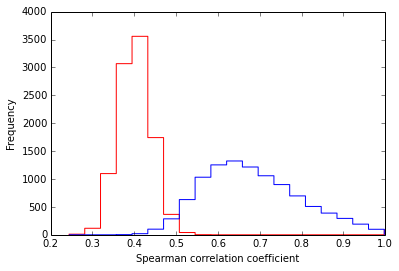
\includegraphics[width=10cm]{local_authorities_files/local_authorities_14_1.png}\end{center}
        \caption{Histogram of Spearman correlations between local positivity and estimated prevalence, calculated at each of 10000 parameter samples.}
        \label{}
    \end{figure}
    
    For the samples drawn, the correlation between prevalence and positivity
(measured by Spearman's \(\rho\)) was always positive and statistically
significant (\(p<0.05\)). However, the correlations - especially for
women - were sometimes weak (see histograms).

As a consistency check, we calculate weighted averages of the prevalence
estimates by LA, and compare these to estimates made from the aggregated
national numbers of tests and diagnoses.

    \begin{footnotesize}
        \begin{Verbatim}[commandchars=\\\{\}]
{\color{incolor}In [{\color{incolor}9}]:} \PY{c}{\PYZsh{} Figure 4}
        
        \PY{n}{pop\PYZus{}active\PYZus{}m} \PY{o}{=} \PY{n}{empty}\PY{p}{(}\PY{p}{[}\PY{n}{n\PYZus{}sample}\PY{p}{,}\PY{n+nb}{len}\PY{p}{(}\PY{n}{alldata}\PY{o}{.}\PY{n}{index}\PY{p}{)}\PY{p}{]}\PY{p}{)}
        \PY{n}{pop\PYZus{}active\PYZus{}f} \PY{o}{=} \PY{n}{empty}\PY{p}{(}\PY{p}{[}\PY{n}{n\PYZus{}sample}\PY{p}{,}\PY{n+nb}{len}\PY{p}{(}\PY{n}{alldata}\PY{o}{.}\PY{n}{index}\PY{p}{)}\PY{p}{]}\PY{p}{)}
        
        \PY{k}{for} \PY{n}{i} \PY{o+ow}{in} \PY{n+nb}{xrange}\PY{p}{(}\PY{n+nb}{len}\PY{p}{(}\PY{n}{alldata}\PY{o}{.}\PY{n}{index}\PY{p}{)}\PY{p}{)}\PY{p}{:}
            \PY{n}{pop\PYZus{}active\PYZus{}m}\PY{p}{[}\PY{p}{:}\PY{p}{,}\PY{n}{i}\PY{p}{]} \PY{o}{=} \PY{n}{rs}\PY{o}{.}\PY{n}{binomial}\PY{p}{(}\PY{n}{alldata}\PY{p}{[}\PY{l+s}{\PYZsq{}}\PY{l+s}{population.male.15\PYZhy{}19}\PY{l+s}{\PYZsq{}}\PY{p}{]}\PY{p}{[}\PY{n}{i}\PY{p}{]} \PYZbs{}
                                            \PY{o}{+} \PY{n}{alldata}\PY{p}{[}\PY{l+s}{\PYZsq{}}\PY{l+s}{population.male.20\PYZhy{}24}\PY{l+s}{\PYZsq{}}\PY{p}{]}\PY{p}{[}\PY{n}{i}\PY{p}{]}\PY{p}{,} 
                                \PY{n}{p\PYZus{}active\PYZus{}m\PYZus{}16\PYZus{}24}\PY{p}{,} \PY{n}{size}\PY{o}{=}\PY{n}{n\PYZus{}sample}\PY{p}{)}
            \PY{n}{pop\PYZus{}active\PYZus{}f}\PY{p}{[}\PY{p}{:}\PY{p}{,}\PY{n}{i}\PY{p}{]} \PY{o}{=} \PY{n}{rs}\PY{o}{.}\PY{n}{binomial}\PY{p}{(}\PY{n}{alldata}\PY{p}{[}\PY{l+s}{\PYZsq{}}\PY{l+s}{population.female.15\PYZhy{}19}\PY{l+s}{\PYZsq{}}\PY{p}{]}\PY{p}{[}\PY{n}{i}\PY{p}{]} \PYZbs{}
                                            \PY{o}{+} \PY{n}{alldata}\PY{p}{[}\PY{l+s}{\PYZsq{}}\PY{l+s}{population.female.20\PYZhy{}24}\PY{l+s}{\PYZsq{}}\PY{p}{]}\PY{p}{[}\PY{n}{i}\PY{p}{]}\PY{p}{,} 
                                \PY{n}{p\PYZus{}active\PYZus{}f\PYZus{}16\PYZus{}24}\PY{p}{,} \PY{n}{size}\PY{o}{=}\PY{n}{n\PYZus{}sample}\PY{p}{)}
            
        \PY{c}{\PYZsh{} testing and diagnosis rates sampled as in england.ipynb}
        \PY{n}{test\PYZus{}rate\PYZus{}m\PYZus{}15\PYZus{}24} \PY{o}{=} \PY{n}{rs}\PY{o}{.}\PY{n}{gamma}\PY{p}{(}\PY{l+m+mi}{566908}\PY{p}{,} \PY{l+m+mi}{1}\PY{p}{,} \PY{n}{size}\PY{o}{=}\PY{n}{n\PYZus{}sample}\PY{p}{)}\PY{o}{/}\PY{n}{pop\PYZus{}active\PYZus{}m\PYZus{}15\PYZus{}24}
        \PY{n}{diag\PYZus{}rate\PYZus{}m\PYZus{}15\PYZus{}24} \PY{o}{=} \PY{n}{rs}\PY{o}{.}\PY{n}{gamma}\PY{p}{(}\PY{l+m+mi}{48387}\PY{p}{,} \PY{l+m+mi}{1}\PY{p}{,} \PY{n}{size}\PY{o}{=}\PY{n}{n\PYZus{}sample}\PY{p}{)}\PY{o}{/}\PY{n}{pop\PYZus{}active\PYZus{}m\PYZus{}15\PYZus{}24}
        \PY{n}{test\PYZus{}rate\PYZus{}f\PYZus{}15\PYZus{}24} \PY{o}{=} \PY{n}{rs}\PY{o}{.}\PY{n}{gamma}\PY{p}{(}\PY{l+m+mi}{1205896}\PY{p}{,} \PY{l+m+mi}{1}\PY{p}{,} \PY{n}{size}\PY{o}{=}\PY{n}{n\PYZus{}sample}\PY{p}{)}\PY{o}{/}\PY{n}{pop\PYZus{}active\PYZus{}f\PYZus{}15\PYZus{}24}
        \PY{n}{diag\PYZus{}rate\PYZus{}f\PYZus{}15\PYZus{}24} \PY{o}{=} \PY{n}{rs}\PY{o}{.}\PY{n}{gamma}\PY{p}{(}\PY{l+m+mi}{88101}\PY{p}{,} \PY{l+m+mi}{1}\PY{p}{,} \PY{n}{size}\PY{o}{=}\PY{n}{n\PYZus{}sample}\PY{p}{)}\PY{o}{/}\PY{n}{pop\PYZus{}active\PYZus{}f\PYZus{}15\PYZus{}24}
        
        \PY{n}{inc\PYZus{}m} \PY{o}{=} \PY{n}{empty}\PY{p}{(}\PY{n}{n\PYZus{}sample}\PY{p}{)}\PY{p}{;} \PY{n}{scr\PYZus{}m} \PY{o}{=} \PY{n}{empty}\PY{p}{(}\PY{n}{n\PYZus{}sample}\PY{p}{)}\PY{p}{;} \PY{n}{prev\PYZus{}m} \PY{o}{=} \PY{n}{empty}\PY{p}{(}\PY{n}{n\PYZus{}sample}\PY{p}{)}\PY{p}{;} 
        \PY{n}{inc\PYZus{}f} \PY{o}{=} \PY{n}{empty}\PY{p}{(}\PY{n}{n\PYZus{}sample}\PY{p}{)}\PY{p}{;} \PY{n}{scr\PYZus{}f} \PY{o}{=} \PY{n}{empty}\PY{p}{(}\PY{n}{n\PYZus{}sample}\PY{p}{)}\PY{p}{;} \PY{n}{prev\PYZus{}f} \PY{o}{=} \PY{n}{empty}\PY{p}{(}\PY{n}{n\PYZus{}sample}\PY{p}{)}\PY{p}{;} 
        
        \PY{k}{for} \PY{n}{j} \PY{o+ow}{in} \PY{n+nb}{xrange}\PY{p}{(}\PY{n}{n\PYZus{}sample}\PY{p}{)}\PY{p}{:}
            \PY{c}{\PYZsh{} local screening and incidence, given local testing and diagnoses}
            \PY{p}{[}\PY{n}{inc\PYZus{}m}\PY{p}{[}\PY{n}{j}\PY{p}{]}\PY{p}{,} \PY{n}{scr\PYZus{}m}\PY{p}{[}\PY{n}{j}\PY{p}{]}\PY{p}{]} \PY{o}{=} \PY{n}{fsolve}\PY{p}{(}\PY{k}{lambda} \PY{n}{x}\PY{p}{:} \PY{n}{test\PYZus{}diag\PYZus{}fun}\PY{p}{(}\PY{n}{concatenate}\PY{p}{(}\PY{p}{[}
                            \PY{n}{x}\PY{p}{,} \PY{n}{array}\PY{p}{(}\PY{p}{[}
                                    \PY{l+m+mi}{1}\PY{o}{\PYZhy{}}\PY{n}{p\PYZus{}asymp\PYZus{}m}\PY{p}{[}\PY{n}{j}\PY{p}{]}\PY{p}{,} \PY{c}{\PYZsh{} proportion of incident infections which are symptomatic}
                                    \PY{n}{sc\PYZus{}m}\PY{p}{[}\PY{n}{j}\PY{p}{]}\PY{p}{,} \PY{c}{\PYZsh{} rate of self\PYZhy{}clear }
                                    \PY{n}{att\PYZus{}symp}\PY{p}{[}\PY{n}{j}\PY{p}{]}\PY{p}{,}
                                    \PY{n}{p\PYZus{}true\PYZus{}pos\PYZus{}m}\PY{p}{[}\PY{n}{j}\PY{p}{]}\PY{p}{,} 
                                    \PY{n}{p\PYZus{}false\PYZus{}pos\PYZus{}m}\PY{p}{[}\PY{n}{j}\PY{p}{]}
                                \PY{p}{]}\PY{p}{)}\PY{p}{]}\PY{p}{)}\PY{p}{)} \PY{o}{\PYZhy{}} \PY{n}{array}\PY{p}{(}\PY{p}{[}\PY{n}{test\PYZus{}rate\PYZus{}m\PYZus{}15\PYZus{}24}\PY{p}{[}\PY{n}{j}\PY{p}{]}\PY{p}{,}\PY{n}{diag\PYZus{}rate\PYZus{}m\PYZus{}15\PYZus{}24}\PY{p}{[}\PY{n}{j}\PY{p}{]}\PY{p}{]}\PY{p}{)}\PY{p}{,} \PY{p}{[}\PY{l+m+mf}{0.09}\PY{p}{,} \PY{l+m+mf}{0.25}\PY{p}{]}\PY{p}{)}
            \PY{c}{\PYZsh{} local prevalence, calculated from local screening and incidence}
            \PY{n}{prev\PYZus{}m}\PY{p}{[}\PY{n}{j}\PY{p}{]} \PY{o}{=} \PY{n}{dyn\PYZus{}fun}\PY{p}{(}
                \PY{n}{inc\PYZus{}m}\PY{p}{[}\PY{n}{j}\PY{p}{]}\PY{o}{*}\PY{n}{p\PYZus{}asymp\PYZus{}m}\PY{p}{[}\PY{n}{j}\PY{p}{]}\PY{p}{,} 
                \PY{n}{sc\PYZus{}m}\PY{p}{[}\PY{n}{j}\PY{p}{]} \PY{o}{+} \PY{n}{scr\PYZus{}m}\PY{p}{[}\PY{n}{j}\PY{p}{]}\PY{o}{*}\PY{n}{p\PYZus{}true\PYZus{}pos\PYZus{}m}\PY{p}{[}\PY{n}{j}\PY{p}{]}\PY{p}{,} 
                \PY{n}{inc\PYZus{}m}\PY{p}{[}\PY{n}{j}\PY{p}{]}\PY{o}{*}\PY{p}{(}\PY{l+m+mi}{1}\PY{o}{\PYZhy{}}\PY{n}{p\PYZus{}asymp\PYZus{}m}\PY{p}{[}\PY{n}{j}\PY{p}{]}\PY{p}{)}\PY{p}{,} 
                \PY{n}{scr\PYZus{}m}\PY{p}{[}\PY{n}{j}\PY{p}{]}\PY{o}{*}\PY{n}{p\PYZus{}true\PYZus{}pos\PYZus{}m}\PY{p}{[}\PY{n}{j}\PY{p}{]} \PY{o}{+} \PY{n}{att\PYZus{}symp}\PY{p}{[}\PY{n}{j}\PY{p}{]}\PY{o}{*}\PY{n}{p\PYZus{}true\PYZus{}pos\PYZus{}m}\PY{p}{[}\PY{n}{j}\PY{p}{]}
            \PY{p}{)}
            \PY{c}{\PYZsh{} local screening and incidence, given local testing and diagnoses}
            \PY{p}{[}\PY{n}{inc\PYZus{}f}\PY{p}{[}\PY{n}{j}\PY{p}{]}\PY{p}{,} \PY{n}{scr\PYZus{}f}\PY{p}{[}\PY{n}{j}\PY{p}{]}\PY{p}{]} \PY{o}{=} \PY{n}{fsolve}\PY{p}{(}\PY{k}{lambda} \PY{n}{x}\PY{p}{:} \PY{n}{test\PYZus{}diag\PYZus{}fun}\PY{p}{(}\PY{n}{concatenate}\PY{p}{(}\PY{p}{[}
                            \PY{n}{x}\PY{p}{,} \PY{n}{array}\PY{p}{(}\PY{p}{[}
                                    \PY{l+m+mi}{1}\PY{o}{\PYZhy{}}\PY{n}{p\PYZus{}asymp\PYZus{}f}\PY{p}{[}\PY{n}{j}\PY{p}{]}\PY{p}{,} \PY{c}{\PYZsh{} proportion of incident infections which are symptomatic}
                                    \PY{n}{sc\PYZus{}f}\PY{p}{[}\PY{n}{j}\PY{p}{]}\PY{p}{,} \PY{c}{\PYZsh{} rate of self\PYZhy{}clear }
                                    \PY{n}{att\PYZus{}symp}\PY{p}{[}\PY{n}{j}\PY{p}{]}\PY{p}{,}
                                    \PY{n}{p\PYZus{}true\PYZus{}pos\PYZus{}f}\PY{p}{[}\PY{n}{j}\PY{p}{]}\PY{p}{,} 
                                    \PY{n}{p\PYZus{}false\PYZus{}pos\PYZus{}f}\PY{p}{[}\PY{n}{j}\PY{p}{]}
                                \PY{p}{]}\PY{p}{)}\PY{p}{]}\PY{p}{)}\PY{p}{)} \PY{o}{\PYZhy{}} \PY{n}{array}\PY{p}{(}\PY{p}{[}\PY{n}{test\PYZus{}rate\PYZus{}f\PYZus{}15\PYZus{}24}\PY{p}{[}\PY{n}{j}\PY{p}{]}\PY{p}{,}\PY{n}{diag\PYZus{}rate\PYZus{}f\PYZus{}15\PYZus{}24}\PY{p}{[}\PY{n}{j}\PY{p}{]}\PY{p}{]}\PY{p}{)}\PY{p}{,} \PY{p}{[}\PY{l+m+mf}{0.09}\PY{p}{,} \PY{l+m+mf}{0.25}\PY{p}{]}\PY{p}{)}
            \PY{c}{\PYZsh{} local prevalence, calculated from local screening and incidence}
            \PY{n}{prev\PYZus{}f}\PY{p}{[}\PY{n}{j}\PY{p}{]} \PY{o}{=} \PY{n}{dyn\PYZus{}fun}\PY{p}{(}
                \PY{n}{inc\PYZus{}f}\PY{p}{[}\PY{n}{j}\PY{p}{]}\PY{o}{*}\PY{n}{p\PYZus{}asymp\PYZus{}f}\PY{p}{[}\PY{n}{j}\PY{p}{]}\PY{p}{,} 
                \PY{n}{sc\PYZus{}f}\PY{p}{[}\PY{n}{j}\PY{p}{]} \PY{o}{+} \PY{n}{scr\PYZus{}f}\PY{p}{[}\PY{n}{j}\PY{p}{]}\PY{o}{*}\PY{n}{p\PYZus{}true\PYZus{}pos\PYZus{}f}\PY{p}{[}\PY{n}{j}\PY{p}{]}\PY{p}{,} 
                \PY{n}{inc\PYZus{}f}\PY{p}{[}\PY{n}{j}\PY{p}{]}\PY{o}{*}\PY{p}{(}\PY{l+m+mi}{1}\PY{o}{\PYZhy{}}\PY{n}{p\PYZus{}asymp\PYZus{}f}\PY{p}{[}\PY{n}{j}\PY{p}{]}\PY{p}{)}\PY{p}{,} 
                \PY{n}{sc\PYZus{}f}\PY{p}{[}\PY{n}{j}\PY{p}{]} \PY{o}{+} \PY{n}{scr\PYZus{}f}\PY{p}{[}\PY{n}{j}\PY{p}{]}\PY{o}{*}\PY{n}{p\PYZus{}true\PYZus{}pos\PYZus{}f}\PY{p}{[}\PY{n}{j}\PY{p}{]} \PY{o}{+} \PY{n}{att\PYZus{}symp}\PY{p}{[}\PY{n}{j}\PY{p}{]}\PY{o}{*}\PY{n}{p\PYZus{}true\PYZus{}pos\PYZus{}f}\PY{p}{[}\PY{n}{j}\PY{p}{]}
            \PY{p}{)}
        
        \PY{n}{hm\PYZus{}las}\PY{o}{=}\PY{n}{plt}\PY{o}{.}\PY{n}{hist}\PY{p}{(}
            \PY{n+nb}{sum}\PY{p}{(}\PY{n}{prev\PYZus{}m\PYZus{}la}\PY{o}{*}\PY{n}{pop\PYZus{}active\PYZus{}m}\PY{p}{,} \PY{n}{axis}\PY{o}{=}\PY{l+m+mi}{1}\PY{p}{)}\PY{o}{/}\PY{n+nb}{sum}\PY{p}{(}\PY{n}{pop\PYZus{}active\PYZus{}m}\PY{p}{,} \PY{n}{axis}\PY{o}{=}\PY{l+m+mi}{1}\PY{p}{)}\PY{p}{,} 
            \PY{l+m+mi}{20}\PY{p}{,} \PY{n}{histtype}\PY{o}{=}\PY{l+s}{\PYZsq{}}\PY{l+s}{step}\PY{l+s}{\PYZsq{}}\PY{p}{,} \PY{n}{normed}\PY{o}{=}\PY{l+s}{\PYZsq{}}\PY{l+s}{true}\PY{l+s}{\PYZsq{}}\PY{p}{,}
            \PY{n}{label} \PY{o}{=} \PY{l+s}{\PYZsq{}}\PY{l+s}{men; by LA}\PY{l+s}{\PYZsq{}}\PY{p}{)}
        \PY{n}{hm\PYZus{}total}\PY{o}{=}\PY{n}{plt}\PY{o}{.}\PY{n}{hist}\PY{p}{(}\PY{n}{prev\PYZus{}m}\PY{p}{,} \PY{l+m+mi}{20}\PY{p}{,} \PY{n}{linestyle}\PY{o}{=}\PY{l+s}{\PYZsq{}}\PY{l+s}{dashed}\PY{l+s}{\PYZsq{}}\PY{p}{,} \PY{n}{histtype}\PY{o}{=}\PY{l+s}{\PYZsq{}}\PY{l+s}{step}\PY{l+s}{\PYZsq{}}\PY{p}{,} \PY{n}{normed}\PY{o}{=}\PY{l+s}{\PYZsq{}}\PY{l+s}{true}\PY{l+s}{\PYZsq{}}\PY{p}{,} \PY{n}{color}\PY{o}{=}\PY{l+s}{\PYZsq{}}\PY{l+s}{b}\PY{l+s}{\PYZsq{}}\PY{p}{,}
            \PY{n}{label} \PY{o}{=} \PY{l+s}{\PYZsq{}}\PY{l+s}{men; national}\PY{l+s}{\PYZsq{}}\PY{p}{)}
        \PY{n}{hf\PYZus{}las}\PY{o}{=}\PY{n}{plt}\PY{o}{.}\PY{n}{hist}\PY{p}{(}
            \PY{n+nb}{sum}\PY{p}{(}\PY{n}{prev\PYZus{}f\PYZus{}la}\PY{o}{*}\PY{n}{pop\PYZus{}active\PYZus{}f}\PY{p}{,} \PY{n}{axis}\PY{o}{=}\PY{l+m+mi}{1}\PY{p}{)}\PY{o}{/}\PY{n+nb}{sum}\PY{p}{(}\PY{n}{pop\PYZus{}active\PYZus{}f}\PY{p}{,} \PY{n}{axis}\PY{o}{=}\PY{l+m+mi}{1}\PY{p}{)}\PY{p}{,} 
            \PY{l+m+mi}{20}\PY{p}{,} \PY{n}{histtype}\PY{o}{=}\PY{l+s}{\PYZsq{}}\PY{l+s}{step}\PY{l+s}{\PYZsq{}}\PY{p}{,} \PY{n}{color}\PY{o}{=}\PY{l+s}{\PYZsq{}}\PY{l+s}{r}\PY{l+s}{\PYZsq{}}\PY{p}{,} \PY{n}{normed}\PY{o}{=}\PY{l+s}{\PYZsq{}}\PY{l+s}{true}\PY{l+s}{\PYZsq{}}\PY{p}{,}
            \PY{n}{label} \PY{o}{=} \PY{l+s}{\PYZsq{}}\PY{l+s}{women; by LA}\PY{l+s}{\PYZsq{}}\PY{p}{)}
        \PY{n}{hf\PYZus{}total}\PY{o}{=}\PY{n}{plt}\PY{o}{.}\PY{n}{hist}\PY{p}{(}\PY{n}{prev\PYZus{}f}\PY{p}{,} \PY{l+m+mi}{20}\PY{p}{,} \PY{n}{linestyle}\PY{o}{=}\PY{l+s}{\PYZsq{}}\PY{l+s}{dashed}\PY{l+s}{\PYZsq{}}\PY{p}{,} \PY{n}{histtype}\PY{o}{=}\PY{l+s}{\PYZsq{}}\PY{l+s}{step}\PY{l+s}{\PYZsq{}}\PY{p}{,} \PY{n}{normed}\PY{o}{=}\PY{l+s}{\PYZsq{}}\PY{l+s}{true}\PY{l+s}{\PYZsq{}}\PY{p}{,} \PY{n}{color}\PY{o}{=}\PY{l+s}{\PYZsq{}}\PY{l+s}{r}\PY{l+s}{\PYZsq{}}\PY{p}{,}
            \PY{n}{label} \PY{o}{=} \PY{l+s}{\PYZsq{}}\PY{l+s}{women; national}\PY{l+s}{\PYZsq{}}\PY{p}{)}
        
        \PY{n}{plt}\PY{o}{.}\PY{n}{xlabel}\PY{p}{(}\PY{l+s}{\PYZsq{}}\PY{l+s}{Prevalence}\PY{l+s}{\PYZsq{}}\PY{p}{)}
        \PY{n}{plt}\PY{o}{.}\PY{n}{legend}\PY{p}{(}\PY{p}{)}
\end{Verbatim}
    \end{footnotesize}

    \begin{footnotesize}
            \begin{Verbatim}[commandchars=\\\{\}]
{\color{outcolor}Out[{\color{outcolor}9}]:} <matplotlib.legend.Legend at 0x10b776ed0>
\end{Verbatim}
    \end{footnotesize}
        
    \begin{figure}
        \begin{center}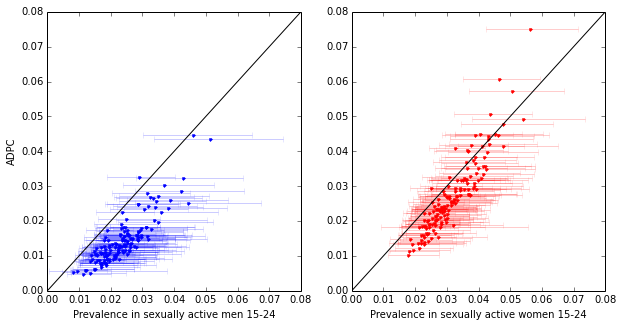
\includegraphics[width=10cm]{local_authorities_files/local_authorities_16_1.png}\end{center}
        \caption{Weighted average of sampled prevalences, by LA (solid lines), and sample based on national numbers of tests and diagnoses (dashed lines).}
        \label{}
    \end{figure}
    
    The sampled prevalence distributions are very close, giving confidence
in our method.

\subsection{Local differences in
prevalence}\label{local-differences-in-prevalence}

We now use our samples to compare prevalence by local authority.

    \begin{footnotesize}
        \begin{Verbatim}[commandchars=\\\{\}]
{\color{incolor}In [{\color{incolor}10}]:} \PY{c}{\PYZsh{} Figure 5}
         
         \PY{n}{fig} \PY{o}{=} \PY{n}{plt}\PY{o}{.}\PY{n}{figure}\PY{p}{(}\PY{n}{figsize} \PY{o}{=} \PY{p}{(}\PY{l+m+mi}{12}\PY{p}{,}\PY{l+m+mi}{3}\PY{p}{)}\PY{p}{)}
         \PY{n}{ax1} \PY{o}{=} \PY{n}{fig}\PY{o}{.}\PY{n}{add\PYZus{}subplot}\PY{p}{(}\PY{l+m+mi}{121}\PY{p}{)}
         \PY{n}{ax2} \PY{o}{=} \PY{n}{fig}\PY{o}{.}\PY{n}{add\PYZus{}subplot}\PY{p}{(}\PY{l+m+mi}{122}\PY{p}{)}
         
         \PY{n}{order\PYZus{}m} \PY{o}{=} \PY{n}{argsort}\PY{p}{(}\PY{n}{percentile}\PY{p}{(}\PY{n}{prev\PYZus{}m\PYZus{}la}\PY{p}{,}\PY{l+m+mi}{50}\PY{p}{,}\PY{n}{axis}\PY{o}{=}\PY{l+m+mi}{0}\PY{p}{)}\PY{p}{)} \PY{c}{\PYZsh{} order by prevalence in men}
         \PY{c}{\PYZsh{} Comment\PYZhy{}out the next line to plot all LAs. You will also need to adjust axis sizes.}
         \PY{n}{order\PYZus{}m} \PY{o}{=} \PY{n}{order\PYZus{}m}\PY{p}{[}\PY{n}{append}\PY{p}{(}\PY{n+nb}{range}\PY{p}{(}\PY{l+m+mi}{0}\PY{p}{,}\PY{l+m+mi}{5}\PY{p}{)}\PY{p}{,}\PY{n+nb}{range}\PY{p}{(}\PY{l+m+mi}{146}\PY{p}{,}\PY{l+m+mi}{151}\PY{p}{)}\PY{p}{)}\PY{p}{]} 
         \PY{n}{ax1}\PY{o}{.}\PY{n}{errorbar}\PY{p}{(}
             \PY{n}{y} \PY{o}{=} \PY{n+nb}{range}\PY{p}{(}\PY{n+nb}{len}\PY{p}{(}\PY{n}{order\PYZus{}m}\PY{p}{)}\PY{p}{)}\PY{p}{,} 
             \PY{n}{x} \PY{o}{=} \PY{p}{(}\PY{n}{percentile}\PY{p}{(}\PY{n}{prev\PYZus{}m\PYZus{}la}\PY{p}{,}\PY{l+m+mi}{50}\PY{p}{,}\PY{n}{axis}\PY{o}{=}\PY{l+m+mi}{0}\PY{p}{)}\PY{p}{)}\PY{p}{[}\PY{n}{order\PYZus{}m}\PY{p}{]}\PY{p}{,} 
             \PY{n}{xerr}\PY{o}{=}\PY{n}{array}\PY{p}{(}\PY{p}{[}\PY{n}{percentile}\PY{p}{(}\PY{n}{prev\PYZus{}m\PYZus{}la}\PY{p}{[}\PY{p}{:}\PY{p}{,}\PY{n}{order\PYZus{}m}\PY{p}{]}\PY{p}{,}\PY{l+m+mi}{50}\PY{p}{,}\PY{n}{axis}\PY{o}{=}\PY{l+m+mi}{0}\PY{p}{)} \PY{o}{\PYZhy{}} \PY{n}{percentile}\PY{p}{(}\PY{n}{prev\PYZus{}m\PYZus{}la}\PY{p}{[}\PY{p}{:}\PY{p}{,}\PY{n}{order\PYZus{}m}\PY{p}{]}\PY{p}{,}\PY{l+m+mf}{2.5}\PY{p}{,}\PY{n}{axis}\PY{o}{=}\PY{l+m+mi}{0}\PY{p}{)}\PY{p}{,}
                     \PY{n}{percentile}\PY{p}{(}\PY{n}{prev\PYZus{}m\PYZus{}la}\PY{p}{[}\PY{p}{:}\PY{p}{,}\PY{n}{order\PYZus{}m}\PY{p}{]}\PY{p}{,}\PY{l+m+mf}{97.5}\PY{p}{,}\PY{n}{axis}\PY{o}{=}\PY{l+m+mi}{0}\PY{p}{)} \PY{o}{\PYZhy{}} \PY{n}{percentile}\PY{p}{(}\PY{n}{prev\PYZus{}m\PYZus{}la}\PY{p}{[}\PY{p}{:}\PY{p}{,}\PY{n}{order\PYZus{}m}\PY{p}{]}\PY{p}{,}\PY{l+m+mi}{50}\PY{p}{,}\PY{n}{axis}\PY{o}{=}\PY{l+m+mi}{0}\PY{p}{)}\PY{p}{]}
                     \PY{p}{)}\PY{p}{,} 
             \PY{n}{fmt}\PY{o}{=}\PY{l+s}{\PYZsq{}}\PY{l+s}{.}\PY{l+s}{\PYZsq{}}\PY{p}{)}
         
         \PY{n}{ax1}\PY{o}{.}\PY{n}{set\PYZus{}ylim}\PY{p}{(}\PY{o}{\PYZhy{}}\PY{l+m+mi}{1}\PY{p}{,} \PY{n+nb}{len}\PY{p}{(}\PY{n}{order\PYZus{}m}\PY{p}{)}\PY{p}{)}\PY{p}{;} \PY{n}{ax1}\PY{o}{.}\PY{n}{set\PYZus{}xlim}\PY{p}{(}\PY{l+m+mi}{0}\PY{p}{,} \PY{l+m+mf}{0.17}\PY{p}{)}
         \PY{n}{ax1}\PY{o}{.}\PY{n}{set\PYZus{}xlabel}\PY{p}{(}\PY{l+s}{\PYZsq{}}\PY{l+s}{Prevalence in sexually active men 15\PYZhy{}24}\PY{l+s}{\PYZsq{}}\PY{p}{)}
         \PY{n}{ax1}\PY{o}{.}\PY{n}{grid}\PY{p}{(}\PY{n+nb+bp}{True}\PY{p}{)}
         \PY{n}{ax1}\PY{o}{.}\PY{n}{set\PYZus{}yticklabels}\PY{p}{(}\PY{p}{[}\PY{p}{]}\PY{p}{)}
         
         \PY{k}{print} \PY{l+s}{\PYZsq{}}\PY{l+s}{Lowest prevalence in men (median sample):}\PY{l+s}{\PYZsq{}}\PY{p}{,} \PY{p}{(}\PY{n}{percentile}\PY{p}{(}\PY{n}{prev\PYZus{}m\PYZus{}la}\PY{p}{,}\PY{l+m+mi}{50}\PY{p}{,}\PY{n}{axis}\PY{o}{=}\PY{l+m+mi}{0}\PY{p}{)}\PY{p}{)}\PY{p}{[}\PY{n}{order\PYZus{}m}\PY{p}{[}\PY{l+m+mi}{0}\PY{p}{]}\PY{p}{]}
         \PY{k}{print} \PY{l+s}{\PYZsq{}}\PY{l+s}{Highest prevalence in men (median sample):}\PY{l+s}{\PYZsq{}}\PY{p}{,} \PY{p}{(}\PY{n}{percentile}\PY{p}{(}\PY{n}{prev\PYZus{}m\PYZus{}la}\PY{p}{,}\PY{l+m+mi}{50}\PY{p}{,}\PY{n}{axis}\PY{o}{=}\PY{l+m+mi}{0}\PY{p}{)}\PY{p}{)}\PY{p}{[}\PY{n}{order\PYZus{}m}\PY{p}{[}\PY{o}{\PYZhy{}}\PY{l+m+mi}{1}\PY{p}{]}\PY{p}{]}
         
         \PY{n}{order\PYZus{}f} \PY{o}{=} \PY{n}{argsort}\PY{p}{(}\PY{n}{percentile}\PY{p}{(}\PY{n}{prev\PYZus{}f\PYZus{}la}\PY{p}{,}\PY{l+m+mi}{50}\PY{p}{,}\PY{n}{axis}\PY{o}{=}\PY{l+m+mi}{0}\PY{p}{)}\PY{p}{)} \PY{c}{\PYZsh{} order by prevalence in women}
         \PY{c}{\PYZsh{} Comment\PYZhy{}out the next line to plot all LAs. You will also need to adjust axis sizes.}
         \PY{n}{order\PYZus{}f} \PY{o}{=} \PY{n}{order\PYZus{}f}\PY{p}{[}\PY{n}{append}\PY{p}{(}\PY{n+nb}{range}\PY{p}{(}\PY{l+m+mi}{0}\PY{p}{,}\PY{l+m+mi}{5}\PY{p}{)}\PY{p}{,}\PY{n+nb}{range}\PY{p}{(}\PY{l+m+mi}{146}\PY{p}{,}\PY{l+m+mi}{151}\PY{p}{)}\PY{p}{)}\PY{p}{]} 
         \PY{n}{ax2}\PY{o}{.}\PY{n}{errorbar}\PY{p}{(}
             \PY{n}{y} \PY{o}{=} \PY{n+nb}{range}\PY{p}{(}\PY{n+nb}{len}\PY{p}{(}\PY{n}{order\PYZus{}f}\PY{p}{)}\PY{p}{)}\PY{p}{,} 
             \PY{n}{x} \PY{o}{=} \PY{p}{(}\PY{n}{percentile}\PY{p}{(}\PY{n}{prev\PYZus{}f\PYZus{}la}\PY{p}{,}\PY{l+m+mi}{50}\PY{p}{,}\PY{n}{axis}\PY{o}{=}\PY{l+m+mi}{0}\PY{p}{)}\PY{p}{)}\PY{p}{[}\PY{n}{order\PYZus{}f}\PY{p}{]}\PY{p}{,} 
             \PY{n}{xerr}\PY{o}{=}\PY{n}{array}\PY{p}{(}\PY{p}{[}\PY{n}{percentile}\PY{p}{(}\PY{n}{prev\PYZus{}f\PYZus{}la}\PY{p}{[}\PY{p}{:}\PY{p}{,}\PY{n}{order\PYZus{}f}\PY{p}{]}\PY{p}{,}\PY{l+m+mi}{50}\PY{p}{,}\PY{n}{axis}\PY{o}{=}\PY{l+m+mi}{0}\PY{p}{)} \PY{o}{\PYZhy{}} \PY{n}{percentile}\PY{p}{(}\PY{n}{prev\PYZus{}f\PYZus{}la}\PY{p}{[}\PY{p}{:}\PY{p}{,}\PY{n}{order\PYZus{}f}\PY{p}{]}\PY{p}{,}\PY{l+m+mf}{2.5}\PY{p}{,}\PY{n}{axis}\PY{o}{=}\PY{l+m+mi}{0}\PY{p}{)}\PY{p}{,}
                     \PY{n}{percentile}\PY{p}{(}\PY{n}{prev\PYZus{}f\PYZus{}la}\PY{p}{[}\PY{p}{:}\PY{p}{,}\PY{n}{order\PYZus{}f}\PY{p}{]}\PY{p}{,}\PY{l+m+mf}{97.5}\PY{p}{,}\PY{n}{axis}\PY{o}{=}\PY{l+m+mi}{0}\PY{p}{)} \PY{o}{\PYZhy{}} \PY{n}{percentile}\PY{p}{(}\PY{n}{prev\PYZus{}f\PYZus{}la}\PY{p}{[}\PY{p}{:}\PY{p}{,}\PY{n}{order\PYZus{}f}\PY{p}{]}\PY{p}{,}\PY{l+m+mi}{50}\PY{p}{,}\PY{n}{axis}\PY{o}{=}\PY{l+m+mi}{0}\PY{p}{)}\PY{p}{]}
                     \PY{p}{)}\PY{p}{,} 
             \PY{n}{color}\PY{o}{=}\PY{l+s}{\PYZsq{}}\PY{l+s}{r}\PY{l+s}{\PYZsq{}}\PY{p}{,}\PY{n}{fmt}\PY{o}{=}\PY{l+s}{\PYZsq{}}\PY{l+s}{.}\PY{l+s}{\PYZsq{}}\PY{p}{)}  
         
         \PY{k}{for} \PY{n}{i} \PY{o+ow}{in} \PY{n+nb}{xrange}\PY{p}{(}\PY{l+m+mi}{10}\PY{p}{)}\PY{p}{:}
             \PY{n}{ax1}\PY{o}{.}\PY{n}{text}\PY{p}{(}\PY{l+m+mf}{0.1}\PY{p}{,} \PY{n}{i}\PY{p}{,} \PY{n}{alldata}\PY{o}{.}\PY{n}{la}\PY{p}{[}\PY{n}{order\PYZus{}m}\PY{p}{[}\PY{n}{i}\PY{p}{]}\PY{p}{]}\PY{p}{)}
             \PY{n}{ax2}\PY{o}{.}\PY{n}{text}\PY{p}{(}\PY{l+m+mf}{0.1}\PY{p}{,} \PY{n}{i}\PY{p}{,} \PY{n}{alldata}\PY{o}{.}\PY{n}{la}\PY{p}{[}\PY{n}{order\PYZus{}f}\PY{p}{[}\PY{n}{i}\PY{p}{]}\PY{p}{]}\PY{p}{)}
         
         \PY{n}{ax2}\PY{o}{.}\PY{n}{set\PYZus{}ylim}\PY{p}{(}\PY{o}{\PYZhy{}}\PY{l+m+mi}{1}\PY{p}{,} \PY{n+nb}{len}\PY{p}{(}\PY{n}{order\PYZus{}f}\PY{p}{)}\PY{p}{)}\PY{p}{;} \PY{n}{ax2}\PY{o}{.}\PY{n}{set\PYZus{}xlim}\PY{p}{(}\PY{l+m+mi}{0}\PY{p}{,} \PY{l+m+mf}{0.17}\PY{p}{)}
         \PY{n}{ax2}\PY{o}{.}\PY{n}{set\PYZus{}xlabel}\PY{p}{(}\PY{l+s}{\PYZsq{}}\PY{l+s}{Prevalence in sexually active women 15\PYZhy{}24}\PY{l+s}{\PYZsq{}}\PY{p}{)}
         \PY{n}{ax2}\PY{o}{.}\PY{n}{grid}\PY{p}{(}\PY{n+nb+bp}{True}\PY{p}{)}
         \PY{n}{ax2}\PY{o}{.}\PY{n}{set\PYZus{}yticklabels}\PY{p}{(}\PY{p}{[}\PY{p}{]}\PY{p}{)}
         
         \PY{k}{print} \PY{l+s}{\PYZsq{}}\PY{l+s}{Lowest prevalence in women (median sample):}\PY{l+s}{\PYZsq{}}\PY{p}{,} \PY{p}{(}\PY{n}{percentile}\PY{p}{(}\PY{n}{prev\PYZus{}f\PYZus{}la}\PY{p}{,}\PY{l+m+mi}{50}\PY{p}{,}\PY{n}{axis}\PY{o}{=}\PY{l+m+mi}{0}\PY{p}{)}\PY{p}{)}\PY{p}{[}\PY{n}{order\PYZus{}f}\PY{p}{[}\PY{l+m+mi}{0}\PY{p}{]}\PY{p}{]}
         \PY{k}{print} \PY{l+s}{\PYZsq{}}\PY{l+s}{Highest prevalence in women (median sample):}\PY{l+s}{\PYZsq{}}\PY{p}{,} \PY{p}{(}\PY{n}{percentile}\PY{p}{(}\PY{n}{prev\PYZus{}f\PYZus{}la}\PY{p}{,}\PY{l+m+mi}{50}\PY{p}{,}\PY{n}{axis}\PY{o}{=}\PY{l+m+mi}{0}\PY{p}{)}\PY{p}{)}\PY{p}{[}\PY{n}{order\PYZus{}f}\PY{p}{[}\PY{o}{\PYZhy{}}\PY{l+m+mi}{1}\PY{p}{]}\PY{p}{]}
\end{Verbatim}
    \end{footnotesize}

    \begin{Verbatim}[commandchars=\\\{\}]
Lowest prevalence in men (median sample): 0.00819755429809
Highest prevalence in men (median sample): 0.0513318116948
Lowest prevalence in women (median sample): 0.0178619507471
Highest prevalence in women (median sample): 0.0561422126184
    \end{Verbatim}

    \begin{figure}
        \begin{center}\adjustimage{max size={0.9\linewidth}{0.4\paperheight}}{local_authorities_files/local_authorities_18_1.png}\end{center}
        \caption{Median and central 95\% credible intervals for chlamydia prevalence in the LAs with the five highest and five lowest estimated prevalences for men (left) and women (right).}
        \label{}
    \end{figure}
    
    In general, the 95\% credible intervals for the highest and lowest LAs
do not overlap at all, or only slightly. However, there are over 100 LAs
with intermediate prevalence in which the distributions do overlap. (A
plot showing all LAs can be obtained by commenting-out the lines
indicated above.) Although there are local differences in prevalence,
they are generally small compared with the uncertainty in our estimates.
Only in the most extreme cases can differences be clearly resolved.

We also plot inferred prevalence against deprivation (rank of average
score from the English Indices of Deprivation 2010):

    \begin{footnotesize}
        \begin{Verbatim}[commandchars=\\\{\}]
{\color{incolor}In [{\color{incolor}11}]:} \PY{c}{\PYZsh{} Figure 6}
         
         \PY{c}{\PYZsh{} lookup table for local authority coding in NCSP vs deprivation data}
         \PY{c}{\PYZsh{} Contains National Statistics data © Crown copyright and database right 2016}
         \PY{n}{district\PYZus{}key} \PY{o}{=} \PY{n}{pd}\PY{o}{.}\PY{n}{read\PYZus{}csv}\PY{p}{(}\PY{l+s}{\PYZsq{}}\PY{l+s}{LAD12\PYZus{}CTY12\PYZus{}EN\PYZus{}LU.csv}\PY{l+s}{\PYZsq{}}\PY{p}{)}
         
         \PY{c}{\PYZsh{} indices of deprivation downloaded from }
         \PY{c}{\PYZsh{} https://www.gov.uk/government/statistics/english\PYZhy{}indices\PYZhy{}of\PYZhy{}deprivation\PYZhy{}2010 1 December 2010}
         \PY{c}{\PYZsh{} Contains public sector information licensed under the Open Government Licence v3.0; }
         \PY{c}{\PYZsh{} http://www.nationalarchives.gov.uk/doc/open\PYZhy{}government\PYZhy{}licence/version/3/}
         \PY{n}{code\PYZus{}key} \PY{o}{=} \PY{n}{pd}\PY{o}{.}\PY{n}{read\PYZus{}csv}\PY{p}{(}\PY{l+s}{\PYZsq{}}\PY{l+s}{code\PYZus{}equivalents.csv}\PY{l+s}{\PYZsq{}}\PY{p}{)} \PY{c}{\PYZsh{} downloaded from https://data.gov.uk/dataset/local\PYZhy{}authority\PYZhy{}districts\PYZhy{}uk\PYZhy{}2012\PYZhy{}names\PYZhy{}and\PYZhy{}codes 4 January 2016}
         \PY{n}{deprivation} \PY{o}{=} \PY{n}{pd}\PY{o}{.}\PY{n}{read\PYZus{}csv}\PY{p}{(}\PY{l+s}{\PYZsq{}}\PY{l+s}{deprivation\PYZus{}indices\PYZus{}2010.csv}\PY{l+s}{\PYZsq{}}\PY{p}{)} 
         
         \PY{n}{fig} \PY{o}{=} \PY{n}{plt}\PY{o}{.}\PY{n}{figure}\PY{p}{(}\PY{n}{figsize} \PY{o}{=} \PY{p}{(}\PY{l+m+mi}{10}\PY{p}{,}\PY{l+m+mi}{5}\PY{p}{)}\PY{p}{)}
         \PY{n}{ax1} \PY{o}{=} \PY{n}{fig}\PY{o}{.}\PY{n}{add\PYZus{}subplot}\PY{p}{(}\PY{l+m+mi}{121}\PY{p}{)}
         \PY{n}{ax2} \PY{o}{=} \PY{n}{fig}\PY{o}{.}\PY{n}{add\PYZus{}subplot}\PY{p}{(}\PY{l+m+mi}{122}\PY{p}{)}
         
         \PY{n}{quantiles\PYZus{}m} \PY{o}{=} \PY{n}{percentile}\PY{p}{(}\PY{n}{prev\PYZus{}m\PYZus{}la}\PY{p}{,} \PY{p}{[}\PY{l+m+mi}{50}\PY{p}{,}\PY{l+m+mf}{2.5}\PY{p}{,}\PY{l+m+mf}{97.5}\PY{p}{]}\PY{p}{,} \PY{l+m+mi}{0}\PY{p}{)}
         \PY{n}{quantiles\PYZus{}f} \PY{o}{=} \PY{n}{percentile}\PY{p}{(}\PY{n}{prev\PYZus{}f\PYZus{}la}\PY{p}{,} \PY{p}{[}\PY{l+m+mi}{50}\PY{p}{,}\PY{l+m+mf}{2.5}\PY{p}{,}\PY{l+m+mf}{97.5}\PY{p}{]}\PY{p}{,} \PY{l+m+mi}{0}\PY{p}{)}
         
         \PY{k}{for} \PY{n}{i} \PY{o+ow}{in} \PY{n}{deprivation}\PY{o}{.}\PY{n}{index}\PY{p}{:}
             
             \PY{n}{old\PYZus{}code} \PY{o}{=} \PY{n}{deprivation}\PY{p}{[}\PY{l+s}{u\PYZsq{}}\PY{l+s}{LA CODE}\PY{l+s}{\PYZsq{}}\PY{p}{]}\PY{p}{[}\PY{n}{i}\PY{p}{]}
             \PY{n}{new\PYZus{}code} \PY{o}{=} \PY{n}{code\PYZus{}key}\PY{p}{[}\PY{l+s}{\PYZsq{}}\PY{l+s}{Current code}\PY{l+s}{\PYZsq{}}\PY{p}{]}\PY{p}{[}\PY{n}{code\PYZus{}key}\PY{p}{[}\PY{l+s}{\PYZsq{}}\PY{l+s}{Former code}\PY{l+s}{\PYZsq{}}\PY{p}{]} \PY{o}{==} \PY{n}{old\PYZus{}code}\PY{p}{]}\PY{o}{.}\PY{n}{tolist}\PY{p}{(}\PY{p}{)}\PY{p}{[}\PY{l+m+mi}{0}\PY{p}{]}
             
             \PY{c}{\PYZsh{} special case for Northumberland, because a new code was allocated when boundaries changed:}
             \PY{k}{if} \PY{n}{new\PYZus{}code} \PY{o}{==} \PY{l+s}{\PYZsq{}}\PY{l+s}{E06000048}\PY{l+s}{\PYZsq{}}\PY{p}{:} \PY{c}{\PYZsh{} Northumberland}
                 \PY{n}{new\PYZus{}code} \PY{o}{=} \PY{l+s}{\PYZsq{}}\PY{l+s}{E06000057}\PY{l+s}{\PYZsq{}}
             
             \PY{k}{if} \PY{n}{new\PYZus{}code} \PY{o+ow}{in} \PY{n}{alldata}\PY{o}{.}\PY{n}{la\PYZus{}code}\PY{o}{.}\PY{n}{tolist}\PY{p}{(}\PY{p}{)}\PY{p}{:} \PY{c}{\PYZsh{} if LA can be found in NCSP data using new code}
                 \PY{n}{ax1}\PY{o}{.}\PY{n}{plot}\PY{p}{(}\PY{n}{deprivation}\PY{p}{[}\PY{l+s}{u\PYZsq{}}\PY{l+s}{Rank of Average Score}\PY{l+s}{\PYZsq{}}\PY{p}{]}\PY{p}{[}\PY{n}{i}\PY{p}{]}\PY{p}{,}
                         \PY{n}{quantiles\PYZus{}m}\PY{p}{[}\PY{l+m+mi}{0}\PY{p}{]}\PY{p}{[}\PY{n}{where}\PY{p}{(}\PY{n}{alldata}\PY{o}{.}\PY{n}{la\PYZus{}code} \PY{o}{==} \PY{n}{new\PYZus{}code}\PY{p}{)}\PY{p}{]}\PY{p}{,}
                         \PY{l+s}{\PYZsq{}}\PY{l+s}{.b}\PY{l+s}{\PYZsq{}}\PY{p}{)}
                 \PY{n}{ax1}\PY{o}{.}\PY{n}{errorbar}\PY{p}{(}\PY{n}{deprivation}\PY{p}{[}\PY{l+s}{u\PYZsq{}}\PY{l+s}{Rank of Average Score}\PY{l+s}{\PYZsq{}}\PY{p}{]}\PY{p}{[}\PY{n}{i}\PY{p}{]}\PY{p}{,}
                         \PY{n}{quantiles\PYZus{}m}\PY{p}{[}\PY{l+m+mi}{0}\PY{p}{]}\PY{p}{[}\PY{n}{where}\PY{p}{(}\PY{n}{alldata}\PY{o}{.}\PY{n}{la\PYZus{}code} \PY{o}{==} \PY{n}{new\PYZus{}code}\PY{p}{)}\PY{p}{]}\PY{p}{,}
                         \PY{n}{yerr} \PY{o}{=} \PY{n}{array}\PY{p}{(}\PY{p}{[}\PY{p}{(}\PY{n}{quantiles\PYZus{}m}\PY{p}{[}\PY{l+m+mi}{0}\PY{p}{]}\PY{o}{\PYZhy{}}\PY{n}{quantiles\PYZus{}m}\PY{p}{[}\PY{l+m+mi}{1}\PY{p}{]}\PY{p}{)}\PY{p}{[}\PY{n}{where}\PY{p}{(}\PY{n}{alldata}\PY{o}{.}\PY{n}{la\PYZus{}code} \PY{o}{==} \PY{n}{new\PYZus{}code}\PY{p}{)}\PY{p}{]}\PY{p}{,}
                                      \PY{p}{(}\PY{n}{quantiles\PYZus{}m}\PY{p}{[}\PY{l+m+mi}{2}\PY{p}{]}\PY{o}{\PYZhy{}}\PY{n}{quantiles\PYZus{}m}\PY{p}{[}\PY{l+m+mi}{0}\PY{p}{]}\PY{p}{)}\PY{p}{[}\PY{n}{where}\PY{p}{(}\PY{n}{alldata}\PY{o}{.}\PY{n}{la\PYZus{}code} \PY{o}{==} \PY{n}{new\PYZus{}code}\PY{p}{)}\PY{p}{]}\PY{p}{]}\PY{p}{)}\PY{p}{,}
                         \PY{n}{color}\PY{o}{=}\PY{l+s}{\PYZsq{}}\PY{l+s}{b}\PY{l+s}{\PYZsq{}}\PY{p}{,} \PY{n}{alpha}\PY{o}{=}\PY{l+m+mf}{0.2}\PY{p}{)}
                 \PY{n}{ax2}\PY{o}{.}\PY{n}{plot}\PY{p}{(}\PY{n}{deprivation}\PY{p}{[}\PY{l+s}{u\PYZsq{}}\PY{l+s}{Rank of Average Score}\PY{l+s}{\PYZsq{}}\PY{p}{]}\PY{p}{[}\PY{n}{i}\PY{p}{]}\PY{p}{,}
                         \PY{n}{quantiles\PYZus{}f}\PY{p}{[}\PY{l+m+mi}{0}\PY{p}{]}\PY{p}{[}\PY{n}{where}\PY{p}{(}\PY{n}{alldata}\PY{o}{.}\PY{n}{la\PYZus{}code} \PY{o}{==} \PY{n}{new\PYZus{}code}\PY{p}{)}\PY{p}{]}\PY{p}{,}
                         \PY{l+s}{\PYZsq{}}\PY{l+s}{.r}\PY{l+s}{\PYZsq{}}\PY{p}{)}
                 \PY{n}{ax2}\PY{o}{.}\PY{n}{errorbar}\PY{p}{(}\PY{n}{deprivation}\PY{p}{[}\PY{l+s}{u\PYZsq{}}\PY{l+s}{Rank of Average Score}\PY{l+s}{\PYZsq{}}\PY{p}{]}\PY{p}{[}\PY{n}{i}\PY{p}{]}\PY{p}{,}
                         \PY{n}{quantiles\PYZus{}f}\PY{p}{[}\PY{l+m+mi}{0}\PY{p}{]}\PY{p}{[}\PY{n}{where}\PY{p}{(}\PY{n}{alldata}\PY{o}{.}\PY{n}{la\PYZus{}code} \PY{o}{==} \PY{n}{new\PYZus{}code}\PY{p}{)}\PY{p}{]}\PY{p}{,}
                         \PY{n}{yerr} \PY{o}{=} \PY{n}{array}\PY{p}{(}\PY{p}{[}\PY{p}{(}\PY{n}{quantiles\PYZus{}f}\PY{p}{[}\PY{l+m+mi}{0}\PY{p}{]}\PY{o}{\PYZhy{}}\PY{n}{quantiles\PYZus{}f}\PY{p}{[}\PY{l+m+mi}{1}\PY{p}{]}\PY{p}{)}\PY{p}{[}\PY{n}{where}\PY{p}{(}\PY{n}{alldata}\PY{o}{.}\PY{n}{la\PYZus{}code} \PY{o}{==} \PY{n}{new\PYZus{}code}\PY{p}{)}\PY{p}{]}\PY{p}{,}
                                      \PY{p}{(}\PY{n}{quantiles\PYZus{}f}\PY{p}{[}\PY{l+m+mi}{2}\PY{p}{]}\PY{o}{\PYZhy{}}\PY{n}{quantiles\PYZus{}f}\PY{p}{[}\PY{l+m+mi}{0}\PY{p}{]}\PY{p}{)}\PY{p}{[}\PY{n}{where}\PY{p}{(}\PY{n}{alldata}\PY{o}{.}\PY{n}{la\PYZus{}code} \PY{o}{==} \PY{n}{new\PYZus{}code}\PY{p}{)}\PY{p}{]}\PY{p}{]}\PY{p}{)}\PY{p}{,}
                         \PY{n}{color}\PY{o}{=}\PY{l+s}{\PYZsq{}}\PY{l+s}{r}\PY{l+s}{\PYZsq{}}\PY{p}{,} \PY{n}{alpha}\PY{o}{=}\PY{l+m+mf}{0.2}\PY{p}{)}
             \PY{k}{elif} \PY{n}{old\PYZus{}code} \PY{o+ow}{in} \PY{n}{district\PYZus{}key}\PY{p}{[}\PY{l+s}{\PYZsq{}}\PY{l+s}{LAD12CDO}\PY{l+s}{\PYZsq{}}\PY{p}{]}\PY{o}{.}\PY{n}{tolist}\PY{p}{(}\PY{p}{)}\PY{p}{:} \PY{c}{\PYZsh{} if LA can be found in list of districts}
                 \PY{n}{new\PYZus{}code} \PY{o}{=} \PY{n}{district\PYZus{}key}\PY{p}{[}\PY{l+s}{\PYZsq{}}\PY{l+s}{CTY12CD}\PY{l+s}{\PYZsq{}}\PY{p}{]}\PY{p}{[}\PY{n}{district\PYZus{}key}\PY{p}{[}\PY{l+s}{\PYZsq{}}\PY{l+s}{LAD12CDO}\PY{l+s}{\PYZsq{}}\PY{p}{]}\PY{o}{==}\PY{n}{old\PYZus{}code}\PY{p}{]}\PY{o}{.}\PY{n}{tolist}\PY{p}{(}\PY{p}{)}\PY{p}{[}\PY{l+m+mi}{0}\PY{p}{]}
                 \PY{c}{\PYZsh{} special case for Gateshead, because a new code was allocated when boundaries changed:}
                 \PY{k}{if} \PY{n}{old\PYZus{}code} \PY{o}{==} \PY{l+s}{\PYZsq{}}\PY{l+s}{00CH}\PY{l+s}{\PYZsq{}}\PY{p}{:}
                     \PY{n}{new\PYZus{}code} \PY{o}{=} \PY{l+s}{\PYZsq{}}\PY{l+s}{E08000037}\PY{l+s}{\PYZsq{}}
                 \PY{n}{ax1}\PY{o}{.}\PY{n}{plot}\PY{p}{(}\PY{n}{deprivation}\PY{p}{[}\PY{l+s}{u\PYZsq{}}\PY{l+s}{Rank of Average Score}\PY{l+s}{\PYZsq{}}\PY{p}{]}\PY{p}{[}\PY{n}{i}\PY{p}{]}\PY{p}{,}
                     \PY{n}{quantiles\PYZus{}m}\PY{p}{[}\PY{l+m+mi}{0}\PY{p}{]}\PY{p}{[}\PY{n}{where}\PY{p}{(}\PY{n}{alldata}\PY{o}{.}\PY{n}{la\PYZus{}code} \PY{o}{==} \PY{n}{new\PYZus{}code}\PY{p}{)}\PY{p}{]}\PY{p}{,}
                     \PY{l+s}{\PYZsq{}}\PY{l+s}{.b}\PY{l+s}{\PYZsq{}}\PY{p}{)} 
                 \PY{n}{ax1}\PY{o}{.}\PY{n}{errorbar}\PY{p}{(}\PY{n}{deprivation}\PY{p}{[}\PY{l+s}{u\PYZsq{}}\PY{l+s}{Rank of Average Score}\PY{l+s}{\PYZsq{}}\PY{p}{]}\PY{p}{[}\PY{n}{i}\PY{p}{]}\PY{p}{,}
                         \PY{n}{quantiles\PYZus{}m}\PY{p}{[}\PY{l+m+mi}{0}\PY{p}{]}\PY{p}{[}\PY{n}{where}\PY{p}{(}\PY{n}{alldata}\PY{o}{.}\PY{n}{la\PYZus{}code} \PY{o}{==} \PY{n}{new\PYZus{}code}\PY{p}{)}\PY{p}{]}\PY{p}{,}
                         \PY{n}{yerr} \PY{o}{=} \PY{n}{array}\PY{p}{(}\PY{p}{[}\PY{p}{(}\PY{n}{quantiles\PYZus{}m}\PY{p}{[}\PY{l+m+mi}{0}\PY{p}{]}\PY{o}{\PYZhy{}}\PY{n}{quantiles\PYZus{}m}\PY{p}{[}\PY{l+m+mi}{1}\PY{p}{]}\PY{p}{)}\PY{p}{[}\PY{n}{where}\PY{p}{(}\PY{n}{alldata}\PY{o}{.}\PY{n}{la\PYZus{}code} \PY{o}{==} \PY{n}{new\PYZus{}code}\PY{p}{)}\PY{p}{]}\PY{p}{,}
                                      \PY{p}{(}\PY{n}{quantiles\PYZus{}m}\PY{p}{[}\PY{l+m+mi}{2}\PY{p}{]}\PY{o}{\PYZhy{}}\PY{n}{quantiles\PYZus{}m}\PY{p}{[}\PY{l+m+mi}{0}\PY{p}{]}\PY{p}{)}\PY{p}{[}\PY{n}{where}\PY{p}{(}\PY{n}{alldata}\PY{o}{.}\PY{n}{la\PYZus{}code} \PY{o}{==} \PY{n}{new\PYZus{}code}\PY{p}{)}\PY{p}{]}\PY{p}{]}\PY{p}{)}\PY{p}{,}
                         \PY{n}{color}\PY{o}{=}\PY{l+s}{\PYZsq{}}\PY{l+s}{b}\PY{l+s}{\PYZsq{}}\PY{p}{,} \PY{n}{alpha}\PY{o}{=}\PY{l+m+mf}{0.2}\PY{p}{)}
                 \PY{n}{ax2}\PY{o}{.}\PY{n}{plot}\PY{p}{(}\PY{n}{deprivation}\PY{p}{[}\PY{l+s}{u\PYZsq{}}\PY{l+s}{Rank of Average Score}\PY{l+s}{\PYZsq{}}\PY{p}{]}\PY{p}{[}\PY{n}{i}\PY{p}{]}\PY{p}{,}
                     \PY{n}{quantiles\PYZus{}f}\PY{p}{[}\PY{l+m+mi}{0}\PY{p}{]}\PY{p}{[}\PY{n}{where}\PY{p}{(}\PY{n}{alldata}\PY{o}{.}\PY{n}{la\PYZus{}code} \PY{o}{==} \PY{n}{new\PYZus{}code}\PY{p}{)}\PY{p}{]}\PY{p}{,}
                     \PY{l+s}{\PYZsq{}}\PY{l+s}{.r}\PY{l+s}{\PYZsq{}}\PY{p}{)}            
                 \PY{n}{ax2}\PY{o}{.}\PY{n}{errorbar}\PY{p}{(}\PY{n}{deprivation}\PY{p}{[}\PY{l+s}{u\PYZsq{}}\PY{l+s}{Rank of Average Score}\PY{l+s}{\PYZsq{}}\PY{p}{]}\PY{p}{[}\PY{n}{i}\PY{p}{]}\PY{p}{,}
                         \PY{n}{quantiles\PYZus{}f}\PY{p}{[}\PY{l+m+mi}{0}\PY{p}{]}\PY{p}{[}\PY{n}{where}\PY{p}{(}\PY{n}{alldata}\PY{o}{.}\PY{n}{la\PYZus{}code} \PY{o}{==} \PY{n}{new\PYZus{}code}\PY{p}{)}\PY{p}{]}\PY{p}{,}
                         \PY{n}{yerr} \PY{o}{=} \PY{n}{array}\PY{p}{(}\PY{p}{[}\PY{p}{(}\PY{n}{quantiles\PYZus{}f}\PY{p}{[}\PY{l+m+mi}{0}\PY{p}{]}\PY{o}{\PYZhy{}}\PY{n}{quantiles\PYZus{}f}\PY{p}{[}\PY{l+m+mi}{1}\PY{p}{]}\PY{p}{)}\PY{p}{[}\PY{n}{where}\PY{p}{(}\PY{n}{alldata}\PY{o}{.}\PY{n}{la\PYZus{}code} \PY{o}{==} \PY{n}{new\PYZus{}code}\PY{p}{)}\PY{p}{]}\PY{p}{,}
                                      \PY{p}{(}\PY{n}{quantiles\PYZus{}f}\PY{p}{[}\PY{l+m+mi}{2}\PY{p}{]}\PY{o}{\PYZhy{}}\PY{n}{quantiles\PYZus{}f}\PY{p}{[}\PY{l+m+mi}{0}\PY{p}{]}\PY{p}{)}\PY{p}{[}\PY{n}{where}\PY{p}{(}\PY{n}{alldata}\PY{o}{.}\PY{n}{la\PYZus{}code} \PY{o}{==} \PY{n}{new\PYZus{}code}\PY{p}{)}\PY{p}{]}\PY{p}{]}\PY{p}{)}\PY{p}{,}
                         \PY{n}{color}\PY{o}{=}\PY{l+s}{\PYZsq{}}\PY{l+s}{r}\PY{l+s}{\PYZsq{}}\PY{p}{,} \PY{n}{alpha}\PY{o}{=}\PY{l+m+mf}{0.2}\PY{p}{)}
             \PY{k}{else}\PY{p}{:} 
                 \PY{c}{\PYZsh{} Scilly Isles not plotted because excluded due to low numbers}
                 \PY{k}{print} \PY{l+s}{\PYZsq{}}\PY{l+s}{no}\PY{l+s}{\PYZsq{}}\PY{p}{,} \PY{n}{deprivation}\PY{p}{[}\PY{l+s}{u\PYZsq{}}\PY{l+s}{LA NAME}\PY{l+s}{\PYZsq{}}\PY{p}{]}\PY{p}{[}\PY{n}{i}\PY{p}{]}\PY{p}{,} \PY{n}{old\PYZus{}code}\PY{p}{,} \PY{n}{new\PYZus{}code} 
             
         \PY{n}{ax1}\PY{o}{.}\PY{n}{set\PYZus{}xlim}\PY{p}{(}\PY{p}{[}\PY{l+m+mi}{0}\PY{p}{,}\PY{l+m+mi}{350}\PY{p}{]}\PY{p}{)}\PY{p}{;} \PY{n}{ax1}\PY{o}{.}\PY{n}{set\PYZus{}ylim}\PY{p}{(}\PY{p}{[}\PY{l+m+mi}{0}\PY{p}{,}\PY{l+m+mf}{0.07}\PY{p}{]}\PY{p}{)}
         \PY{n}{ax1}\PY{o}{.}\PY{n}{set\PYZus{}xlabel}\PY{p}{(}\PY{l+s}{\PYZsq{}}\PY{l+s}{Index of Multiple Deprivation}\PY{l+s}{\PYZsq{}}\PY{p}{)}
         \PY{n}{ax1}\PY{o}{.}\PY{n}{set\PYZus{}ylabel}\PY{p}{(}\PY{l+s}{\PYZsq{}}\PY{l+s}{Prevalence in sexually active 15\PYZhy{}24\PYZhy{}year\PYZhy{}olds}\PY{l+s}{\PYZsq{}}\PY{p}{)}
         \PY{c}{\PYZsh{}ax1.set\PYZus{}title(\PYZsq{}Sexually active men 15\PYZhy{}24 years\PYZsq{})}
         \PY{n}{ax2}\PY{o}{.}\PY{n}{set\PYZus{}xlim}\PY{p}{(}\PY{p}{[}\PY{l+m+mi}{0}\PY{p}{,}\PY{l+m+mi}{350}\PY{p}{]}\PY{p}{)}\PY{p}{;} \PY{n}{ax2}\PY{o}{.}\PY{n}{set\PYZus{}ylim}\PY{p}{(}\PY{p}{[}\PY{l+m+mi}{0}\PY{p}{,}\PY{l+m+mf}{0.07}\PY{p}{]}\PY{p}{)}
         \PY{n}{ax2}\PY{o}{.}\PY{n}{set\PYZus{}xlabel}\PY{p}{(}\PY{l+s}{\PYZsq{}}\PY{l+s}{Index of Multiple Deprivation}\PY{l+s}{\PYZsq{}}\PY{p}{)}
         \PY{c}{\PYZsh{}ax2.set\PYZus{}ylabel(\PYZsq{}Prevalence\PYZsq{})}
         \PY{c}{\PYZsh{}ax2.set\PYZus{}title(\PYZsq{}Sexually active women 15\PYZhy{}24 years\PYZsq{})}
\end{Verbatim}
    \end{footnotesize}

    \begin{Verbatim}[commandchars=\\\{\}]
no Isles of Scilly 00HF E06000053
    \end{Verbatim}

    \begin{footnotesize}
            \begin{Verbatim}[commandchars=\\\{\}]
{\color{outcolor}Out[{\color{outcolor}11}]:} <matplotlib.text.Text at 0x113fbfa50>
\end{Verbatim}
    \end{footnotesize}
        
    \begin{figure}
        \begin{center}\adjustimage{max size={0.9\linewidth}{0.4\paperheight}}{local_authorities_files/local_authorities_20_2.png}\end{center}
        \caption{Estimated chlamydia prevalence with rank of average deprivation score (lowest rank is most deprived district), for men (left) and women (right) aged 15-24. Points and error bars give median and central 95\% credible interval sampled prevalence.}
        \label{}
    \end{figure}
    
    The pattern shown, of higher prevalence in more deprived areas, agrees
with primary analysis of Natsal-3 (Sonnenberg \emph{et al.}, 2013) which
identified index of multiple deprivation quintile as a risk factor for
chlamydia infection.

We can also show local prevalence on a map:

    \begin{footnotesize}
        \begin{Verbatim}[commandchars=\\\{\}]
{\color{incolor}In [{\color{incolor}12}]:} \PY{c}{\PYZsh{} Figure 7}
         
         \PY{k+kn}{import} \PY{n+nn}{shapefile}
         \PY{k+kn}{import} \PY{n+nn}{matplotlib.pyplot} \PY{k+kn}{as} \PY{n+nn}{plt}
         \PY{k+kn}{import} \PY{n+nn}{matplotlib.patches} \PY{k+kn}{as} \PY{n+nn}{patches}
         \PY{k+kn}{from} \PY{n+nn}{matplotlib.patches} \PY{k+kn}{import} \PY{n}{Polygon}
         \PY{k+kn}{from} \PY{n+nn}{matplotlib.collections} \PY{k+kn}{import} \PY{n}{PatchCollection}
         \PY{k+kn}{from} \PY{n+nn}{mpl\PYZus{}toolkits.axes\PYZus{}grid1.inset\PYZus{}locator} \PY{k+kn}{import} \PY{n}{inset\PYZus{}axes}
         
         \PY{n}{sf} \PY{o}{=} \PY{n}{shapefile}\PY{o}{.}\PY{n}{Reader}\PY{p}{(}\PY{l+s}{\PYZdq{}}\PY{l+s}{County\PYZus{}and\PYZus{}unitary\PYZus{}authorities\PYZus{}E+W\PYZus{}2013\PYZus{}Boundaries\PYZus{}Generalised\PYZus{}Clipped/CTYUA\PYZus{}DEC\PYZus{}2013\PYZus{}EW\PYZus{}BGC}\PY{l+s}{\PYZdq{}}\PY{p}{)}
         \PY{n}{recs}    \PY{o}{=} \PY{n}{sf}\PY{o}{.}\PY{n}{records}\PY{p}{(}\PY{p}{)}
         \PY{n}{shapes}  \PY{o}{=} \PY{n}{sf}\PY{o}{.}\PY{n}{shapes}\PY{p}{(}\PY{p}{)}
         
         \PY{n}{blues} \PY{o}{=} \PY{n}{plt}\PY{o}{.}\PY{n}{get\PYZus{}cmap}\PY{p}{(}\PY{l+s}{\PYZsq{}}\PY{l+s}{Blues}\PY{l+s}{\PYZsq{}}\PY{p}{)}  \PY{c}{\PYZsh{} this returns a colormap}
         \PY{n}{reds} \PY{o}{=} \PY{n}{plt}\PY{o}{.}\PY{n}{get\PYZus{}cmap}\PY{p}{(}\PY{l+s}{\PYZsq{}}\PY{l+s}{Reds}\PY{l+s}{\PYZsq{}}\PY{p}{)}  \PY{c}{\PYZsh{} this returns a colormap}
         
         \PY{n}{key\PYZus{}ys} \PY{o}{=} \PY{n}{array}\PY{p}{(}\PY{p}{[}\PY{l+m+mf}{5.2}\PY{p}{,} \PY{l+m+mf}{5.6}\PY{p}{,} \PY{l+m+mi}{6}\PY{p}{,} \PY{l+m+mf}{6.4}\PY{p}{,} \PY{l+m+mf}{6.8}\PY{p}{]}\PY{p}{)}\PY{o}{*}\PY{l+m+mi}{10}\PY{o}{*}\PY{o}{*}\PY{l+m+mi}{5} \PY{c}{\PYZsh{} y\PYZhy{}co\PYZhy{}ordinates for key}
         \PY{n}{key\PYZus{}labels} \PY{o}{=} \PY{p}{[}\PY{l+s}{\PYZsq{}}\PY{l+s}{lowest quintile}\PY{l+s}{\PYZsq{}}\PY{p}{,}\PY{l+s}{\PYZsq{}}\PY{l+s}{2nd quintile}\PY{l+s}{\PYZsq{}}\PY{p}{,}\PY{l+s}{\PYZsq{}}\PY{l+s}{3rd quintile}\PY{l+s}{\PYZsq{}}\PY{p}{,}\PY{l+s}{\PYZsq{}}\PY{l+s}{4th quintile}\PY{l+s}{\PYZsq{}}\PY{p}{,}\PY{l+s}{\PYZsq{}}\PY{l+s}{highest prevalence quintile}\PY{l+s}{\PYZsq{}}\PY{p}{]}
         
         \PY{n}{fig} \PY{o}{=} \PY{n}{plt}\PY{o}{.}\PY{n}{figure}\PY{p}{(}\PY{n}{figsize} \PY{o}{=} \PY{p}{(}\PY{l+m+mi}{10}\PY{p}{,}\PY{l+m+mi}{5}\PY{p}{)}\PY{p}{)}
         \PY{n}{ax1} \PY{o}{=} \PY{n}{fig}\PY{o}{.}\PY{n}{add\PYZus{}subplot}\PY{p}{(}\PY{l+m+mi}{121}\PY{p}{)}
         \PY{n}{ains1} \PY{o}{=} \PY{n}{inset\PYZus{}axes}\PY{p}{(}\PY{n}{ax1}\PY{p}{,} \PY{n}{width}\PY{o}{=}\PY{l+s}{\PYZsq{}}\PY{l+s}{40}\PY{l+s}{\PYZpc{}}\PY{l+s}{\PYZsq{}}\PY{p}{,} \PY{n}{height}\PY{o}{=}\PY{l+s}{\PYZsq{}}\PY{l+s}{30}\PY{l+s}{\PYZpc{}}\PY{l+s}{\PYZsq{}}\PY{p}{,} \PY{n}{loc}\PY{o}{=}\PY{l+m+mi}{6}\PY{p}{)}
         \PY{n}{ax2} \PY{o}{=} \PY{n}{fig}\PY{o}{.}\PY{n}{add\PYZus{}subplot}\PY{p}{(}\PY{l+m+mi}{122}\PY{p}{)}
         \PY{n}{ains2} \PY{o}{=} \PY{n}{inset\PYZus{}axes}\PY{p}{(}\PY{n}{ax2}\PY{p}{,} \PY{n}{width}\PY{o}{=}\PY{l+s}{\PYZsq{}}\PY{l+s}{40}\PY{l+s}{\PYZpc{}}\PY{l+s}{\PYZsq{}}\PY{p}{,} \PY{n}{height}\PY{o}{=}\PY{l+s}{\PYZsq{}}\PY{l+s}{30}\PY{l+s}{\PYZpc{}}\PY{l+s}{\PYZsq{}}\PY{p}{,} \PY{n}{loc}\PY{o}{=}\PY{l+m+mi}{6}\PY{p}{)}
         
         \PY{n}{n\PYZus{}quantile} \PY{o}{=} \PY{l+m+mi}{5} \PY{c}{\PYZsh{} how many different colours do you want to plot?}
         
         \PY{k}{def} \PY{n+nf}{tickpar}\PY{p}{(}\PY{n}{ax}\PY{p}{)}\PY{p}{:}
             \PY{n}{ax}\PY{o}{.}\PY{n}{tick\PYZus{}params}\PY{p}{(}
                 \PY{n}{axis}\PY{o}{=}\PY{l+s}{\PYZsq{}}\PY{l+s}{both}\PY{l+s}{\PYZsq{}}\PY{p}{,} \PY{c}{\PYZsh{} changes apply to }
                 \PY{n}{which}\PY{o}{=}\PY{l+s}{\PYZsq{}}\PY{l+s}{both}\PY{l+s}{\PYZsq{}}\PY{p}{,} \PY{c}{\PYZsh{} both major and minor ticks are affected}
                 \PY{n}{bottom}\PY{o}{=}\PY{l+s}{\PYZsq{}}\PY{l+s}{off}\PY{l+s}{\PYZsq{}}\PY{p}{,} \PY{c}{\PYZsh{} ticks along the bottom edge are off}
                 \PY{n}{top}\PY{o}{=}\PY{l+s}{\PYZsq{}}\PY{l+s}{off}\PY{l+s}{\PYZsq{}}\PY{p}{,} \PY{c}{\PYZsh{} ticks along the top edge are off}
                 \PY{n}{left}\PY{o}{=}\PY{l+s}{\PYZsq{}}\PY{l+s}{off}\PY{l+s}{\PYZsq{}}\PY{p}{,}      
                 \PY{n}{right}\PY{o}{=}\PY{l+s}{\PYZsq{}}\PY{l+s}{off}\PY{l+s}{\PYZsq{}}\PY{p}{,}         
                 \PY{n}{labelbottom}\PY{o}{=}\PY{l+s}{\PYZsq{}}\PY{l+s}{off}\PY{l+s}{\PYZsq{}}\PY{p}{,}
                 \PY{n}{labelleft}\PY{o}{=}\PY{l+s}{\PYZsq{}}\PY{l+s}{off}\PY{l+s}{\PYZsq{}}\PY{p}{)} \PY{c}{\PYZsh{} labels along the left edge are off}
             
         \PY{c}{\PYZsh{}\PYZsh{}\PYZsh{}\PYZsh{}\PYZsh{}\PYZsh{}\PYZsh{}\PYZsh{}\PYZsh{}\PYZsh{}\PYZsh{}\PYZsh{}\PYZsh{}\PYZsh{}\PYZsh{}\PYZsh{}\PYZsh{}\PYZsh{}\PYZsh{}\PYZsh{}\PYZsh{}\PYZsh{}\PYZsh{}}
         \PY{c}{\PYZsh{} plot prevalence in men}
         \PY{c}{\PYZsh{}\PYZsh{}\PYZsh{}\PYZsh{}\PYZsh{}\PYZsh{}\PYZsh{}\PYZsh{}\PYZsh{}\PYZsh{}\PYZsh{}\PYZsh{}\PYZsh{}\PYZsh{}\PYZsh{}\PYZsh{}\PYZsh{}\PYZsh{}\PYZsh{}\PYZsh{}\PYZsh{}\PYZsh{}\PYZsh{}}
         
         \PY{n}{cNorm}  \PY{o}{=} \PY{n}{plt}\PY{o}{.}\PY{n}{Normalize}\PY{p}{(}\PY{n}{vmin}\PY{o}{=}\PY{l+m+mi}{0}\PY{p}{,} \PY{n}{vmax}\PY{o}{=}\PY{n}{n\PYZus{}quantile}\PY{p}{)}
         \PY{n}{scalarMap} \PY{o}{=} \PY{n}{plt}\PY{o}{.}\PY{n}{cm}\PY{o}{.}\PY{n}{ScalarMappable}\PY{p}{(}\PY{n}{norm}\PY{o}{=}\PY{n}{cNorm}\PY{p}{,} \PY{n}{cmap}\PY{o}{=}\PY{n}{blues}\PY{p}{)}
         \PY{n}{colors} \PY{o}{=} \PY{n}{argsort}\PY{p}{(}\PY{n}{percentile}\PY{p}{(}\PY{n}{prev\PYZus{}m\PYZus{}la}\PY{p}{,}\PY{l+m+mi}{50}\PY{p}{,}\PY{l+m+mi}{0}\PY{p}{)}\PY{p}{)}
         \PY{n}{ranks} \PY{o}{=} \PY{n}{argsort}\PY{p}{(}\PY{n}{colors}\PY{p}{)}
         \PY{c}{\PYZsh{}patches = []}
         
         \PY{k}{for} \PY{n}{nshp} \PY{o+ow}{in} \PY{n}{alldata}\PY{o}{.}\PY{n}{index}\PY{p}{:}
             
            
             \PY{c}{\PYZsh{} code for this LA}
             \PY{n}{thiscode} \PY{o}{=} \PY{n}{alldata}\PY{o}{.}\PY{n}{la\PYZus{}code}\PY{p}{[}\PY{n}{nshp}\PY{p}{]}
             \PY{c}{\PYZsh{} index to find the right shape file for this la:}
             \PY{n}{shpin} \PY{o}{=} \PY{n}{where}\PY{p}{(} \PY{n+nb}{map}\PY{p}{(}\PY{k}{lambda} \PY{n}{x}\PY{p}{:} \PY{n}{thiscode} \PY{o}{==} \PY{n}{x}\PY{p}{,} \PY{p}{[}\PY{n}{recs}\PY{p}{[}\PY{n}{i}\PY{p}{]}\PY{p}{[}\PY{l+m+mi}{0}\PY{p}{]} \PY{k}{for} \PY{n}{i} \PY{o+ow}{in} \PY{n+nb}{range}\PY{p}{(}\PY{n+nb}{len}\PY{p}{(}\PY{n}{recs}\PY{p}{)}\PY{p}{)}\PY{p}{]}\PY{p}{)} \PY{p}{)} 
             \PY{n}{shpin} \PY{o}{=} \PY{n+nb}{int}\PY{p}{(}\PY{n}{shpin}\PY{p}{[}\PY{l+m+mi}{0}\PY{p}{]}\PY{p}{)}
             
             \PY{n}{ptchs}   \PY{o}{=} \PY{p}{[}\PY{p}{]}
             \PY{n}{ptchs\PYZus{}l}   \PY{o}{=} \PY{p}{[}\PY{p}{]} \PY{c}{\PYZsh{} for london}
             \PY{n}{pts}     \PY{o}{=} \PY{n}{array}\PY{p}{(}\PY{n}{shapes}\PY{p}{[}\PY{n}{shpin}\PY{p}{]}\PY{o}{.}\PY{n}{points}\PY{p}{)}
             \PY{n}{prt}     \PY{o}{=} \PY{n}{shapes}\PY{p}{[}\PY{n}{shpin}\PY{p}{]}\PY{o}{.}\PY{n}{parts}
             \PY{n}{par}     \PY{o}{=} \PY{n+nb}{list}\PY{p}{(}\PY{n}{prt}\PY{p}{)} \PY{o}{+} \PY{p}{[}\PY{n}{pts}\PY{o}{.}\PY{n}{shape}\PY{p}{[}\PY{l+m+mi}{0}\PY{p}{]}\PY{p}{]}
             
             \PY{n}{colorVal} \PY{o}{=} \PY{n}{scalarMap}\PY{o}{.}\PY{n}{to\PYZus{}rgba}\PY{p}{(}\PY{n}{n\PYZus{}quantile}\PY{o}{*}\PY{n}{ranks}\PY{p}{[}\PY{n}{nshp}\PY{p}{]}\PY{o}{/}\PY{l+m+mi}{151}\PY{p}{)}
             
             \PY{k}{for} \PY{n}{pij} \PY{o+ow}{in} \PY{n+nb}{xrange}\PY{p}{(}\PY{n+nb}{len}\PY{p}{(}\PY{n}{prt}\PY{p}{)}\PY{p}{)}\PY{p}{:}
                 \PY{n}{ptchs}\PY{o}{.}\PY{n}{append}\PY{p}{(}\PY{n}{Polygon}\PY{p}{(}\PY{n}{pts}\PY{p}{[}\PY{n}{par}\PY{p}{[}\PY{n}{pij}\PY{p}{]}\PY{p}{:}\PY{n}{par}\PY{p}{[}\PY{n}{pij}\PY{o}{+}\PY{l+m+mi}{1}\PY{p}{]}\PY{p}{]}\PY{p}{)}\PY{p}{)}
                 
                 \PY{n}{p} \PY{o}{=} \PY{n}{PatchCollection}\PY{p}{(}\PY{n}{ptchs}\PY{p}{,} \PY{n}{facecolor}\PY{o}{=}\PY{n}{colorVal}\PY{p}{,} \PY{n}{edgecolor}\PY{o}{=}\PY{l+s}{\PYZsq{}}\PY{l+s}{k}\PY{l+s}{\PYZsq{}}\PY{p}{,} \PY{n}{linewidth}\PY{o}{=}\PY{l+m+mf}{0.1}\PY{p}{)}
                 \PY{n}{p}\PY{o}{.}\PY{n}{set\PYZus{}clim}\PY{p}{(}\PY{p}{[}\PY{l+m+mi}{0}\PY{p}{,}\PY{l+m+mi}{151}\PY{p}{]}\PY{p}{)}
                 \PY{n}{ax1}\PY{o}{.}\PY{n}{add\PYZus{}collection}\PY{p}{(}\PY{n}{p}\PY{p}{)}
                 
                 \PY{k}{if} \PY{n}{alldata}\PY{o}{.}\PY{n}{gor}\PY{p}{[}\PY{n}{nshp}\PY{p}{]} \PY{o}{==} \PY{l+s}{\PYZsq{}}\PY{l+s}{london}\PY{l+s}{\PYZsq{}}\PY{p}{:}
                     \PY{n}{p} \PY{o}{=} \PY{n}{PatchCollection}\PY{p}{(}\PY{n}{ptchs}\PY{p}{,} \PY{n}{facecolor}\PY{o}{=}\PY{n}{colorVal}\PY{p}{,} \PY{n}{edgecolor}\PY{o}{=}\PY{l+s}{\PYZsq{}}\PY{l+s}{k}\PY{l+s}{\PYZsq{}}\PY{p}{,} \PY{n}{linewidth}\PY{o}{=}\PY{l+m+mf}{0.1}\PY{p}{)}
                     \PY{n}{ains1}\PY{o}{.}\PY{n}{add\PYZus{}collection}\PY{p}{(}\PY{n}{p}\PY{p}{)}
         
         \PY{k}{for} \PY{n}{i} \PY{o+ow}{in} \PY{n+nb}{xrange}\PY{p}{(}\PY{l+m+mi}{5}\PY{p}{)}\PY{p}{:}
             \PY{n}{ax1}\PY{o}{.}\PY{n}{add\PYZus{}patch}\PY{p}{(}\PY{n}{patches}\PY{o}{.}\PY{n}{Rectangle}\PY{p}{(}\PY{p}{(}\PY{l+m+mf}{0.2}\PY{o}{*}\PY{l+m+mi}{10}\PY{o}{*}\PY{o}{*}\PY{l+m+mi}{5}\PY{p}{,} \PY{n}{key\PYZus{}ys}\PY{p}{[}\PY{n}{i}\PY{p}{]}\PY{p}{)}\PY{p}{,} \PY{l+m+mf}{0.25}\PY{o}{*}\PY{l+m+mi}{10}\PY{o}{*}\PY{o}{*}\PY{l+m+mi}{5}\PY{p}{,} \PY{l+m+mf}{0.25}\PY{o}{*}\PY{l+m+mi}{10}\PY{o}{*}\PY{o}{*}\PY{l+m+mi}{5}\PY{p}{,} \PY{n}{fc}\PY{o}{=}\PY{n}{blues}\PY{p}{(}\PY{l+m+mf}{0.2}\PY{o}{*}\PY{n}{i}\PY{p}{)}\PY{p}{)}\PY{p}{)}
             \PY{n}{ax1}\PY{o}{.}\PY{n}{text}\PY{p}{(}\PY{l+m+mf}{0.6}\PY{o}{*}\PY{l+m+mi}{10}\PY{o}{*}\PY{o}{*}\PY{l+m+mi}{5}\PY{p}{,} \PY{n}{key\PYZus{}ys}\PY{p}{[}\PY{n}{i}\PY{p}{]}\PY{p}{,} \PY{n}{key\PYZus{}labels}\PY{p}{[}\PY{n}{i}\PY{p}{]}\PY{p}{)}
         
         \PY{n}{ax1}\PY{o}{.}\PY{n}{text}\PY{p}{(}\PY{l+m+mf}{0.6}\PY{o}{*}\PY{l+m+mi}{10}\PY{o}{*}\PY{o}{*}\PY{l+m+mi}{5}\PY{p}{,} \PY{l+m+mf}{6.8}\PY{o}{*}\PY{l+m+mi}{10}\PY{o}{*}\PY{o}{*}\PY{l+m+mi}{5}\PY{p}{,} \PY{l+s}{\PYZsq{}}\PY{l+s}{highest prevalence quintile}\PY{l+s}{\PYZsq{}}\PY{p}{)}
         \PY{n}{ax1}\PY{o}{.}\PY{n}{text}\PY{p}{(}\PY{l+m+mf}{0.6}\PY{o}{*}\PY{l+m+mi}{10}\PY{o}{*}\PY{o}{*}\PY{l+m+mi}{5}\PY{p}{,} \PY{l+m+mf}{6.4}\PY{o}{*}\PY{l+m+mi}{10}\PY{o}{*}\PY{o}{*}\PY{l+m+mi}{5}\PY{p}{,} \PY{l+s}{\PYZsq{}}\PY{l+s}{4th quintile}\PY{l+s}{\PYZsq{}}\PY{p}{)}
         \PY{n}{ax1}\PY{o}{.}\PY{n}{text}\PY{p}{(}\PY{l+m+mf}{0.6}\PY{o}{*}\PY{l+m+mi}{10}\PY{o}{*}\PY{o}{*}\PY{l+m+mi}{5}\PY{p}{,} \PY{l+m+mi}{6}\PY{o}{*}\PY{l+m+mi}{10}\PY{o}{*}\PY{o}{*}\PY{l+m+mi}{5}\PY{p}{,} \PY{l+s}{\PYZsq{}}\PY{l+s}{3rd quintile}\PY{l+s}{\PYZsq{}}\PY{p}{)}
         \PY{n}{ax1}\PY{o}{.}\PY{n}{text}\PY{p}{(}\PY{l+m+mf}{0.6}\PY{o}{*}\PY{l+m+mi}{10}\PY{o}{*}\PY{o}{*}\PY{l+m+mi}{5}\PY{p}{,} \PY{l+m+mf}{5.6}\PY{o}{*}\PY{l+m+mi}{10}\PY{o}{*}\PY{o}{*}\PY{l+m+mi}{5}\PY{p}{,} \PY{l+s}{\PYZsq{}}\PY{l+s}{2nd quintile}\PY{l+s}{\PYZsq{}}\PY{p}{)}
         \PY{n}{ax1}\PY{o}{.}\PY{n}{text}\PY{p}{(}\PY{l+m+mf}{0.6}\PY{o}{*}\PY{l+m+mi}{10}\PY{o}{*}\PY{o}{*}\PY{l+m+mi}{5}\PY{p}{,} \PY{l+m+mf}{5.2}\PY{o}{*}\PY{l+m+mi}{10}\PY{o}{*}\PY{o}{*}\PY{l+m+mi}{5}\PY{p}{,} \PY{l+s}{\PYZsq{}}\PY{l+s}{lowest quintile}\PY{l+s}{\PYZsq{}}\PY{p}{)}
         
         \PY{n}{ax1}\PY{o}{.}\PY{n}{set\PYZus{}xlim}\PY{p}{(}\PY{l+m+mi}{0}\PY{p}{,} \PY{l+m+mf}{0.7}\PY{o}{*}\PY{l+m+mi}{10}\PY{o}{*}\PY{o}{*}\PY{l+m+mi}{6}\PY{p}{)}
         \PY{n}{ax1}\PY{o}{.}\PY{n}{set\PYZus{}ylim}\PY{p}{(}\PY{l+m+mi}{0}\PY{p}{,} \PY{l+m+mf}{0.7}\PY{o}{*}\PY{l+m+mi}{10}\PY{o}{*}\PY{o}{*}\PY{l+m+mi}{6}\PY{p}{)}
         \PY{n}{ax1}\PY{o}{.}\PY{n}{set\PYZus{}aspect}\PY{p}{(}\PY{l+s}{\PYZsq{}}\PY{l+s}{equal}\PY{l+s}{\PYZsq{}}\PY{p}{,} \PY{l+s}{\PYZsq{}}\PY{l+s}{datalim}\PY{l+s}{\PYZsq{}}\PY{p}{)}
         \PY{n}{tickpar}\PY{p}{(}\PY{n}{ax1}\PY{p}{)}
         \PY{n}{ains1}\PY{o}{.}\PY{n}{set\PYZus{}xlim}\PY{p}{(}\PY{l+m+mf}{0.5}\PY{o}{*}\PY{l+m+mi}{10}\PY{o}{*}\PY{o}{*}\PY{l+m+mi}{6}\PY{p}{,} \PY{l+m+mf}{0.565}\PY{o}{*}\PY{l+m+mi}{10}\PY{o}{*}\PY{o}{*}\PY{l+m+mi}{6}\PY{p}{)}
         \PY{n}{ains1}\PY{o}{.}\PY{n}{set\PYZus{}ylim}\PY{p}{(}\PY{l+m+mf}{1.55}\PY{o}{*}\PY{l+m+mi}{10}\PY{o}{*}\PY{o}{*}\PY{l+m+mi}{5}\PY{p}{,} \PY{l+m+mf}{2.05}\PY{o}{*}\PY{l+m+mi}{10}\PY{o}{*}\PY{o}{*}\PY{l+m+mi}{5}\PY{p}{)}
         \PY{n}{ains1}\PY{o}{.}\PY{n}{set\PYZus{}aspect}\PY{p}{(}\PY{l+s}{\PYZsq{}}\PY{l+s}{equal}\PY{l+s}{\PYZsq{}}\PY{p}{,} \PY{l+s}{\PYZsq{}}\PY{l+s}{datalim}\PY{l+s}{\PYZsq{}}\PY{p}{)}
         \PY{n}{tickpar}\PY{p}{(}\PY{n}{ains1}\PY{p}{)}
         \PY{n}{p} \PY{o}{=} \PY{n}{PatchCollection}\PY{p}{(}\PY{n}{ptchs}\PY{p}{,} \PY{n}{cmap}\PY{o}{=}\PY{n}{blues}\PY{p}{)}
         \PY{n}{p} \PY{o}{=} \PY{n}{PatchCollection}\PY{p}{(}\PY{n}{ptchs\PYZus{}l}\PY{p}{,} \PY{n}{cmap}\PY{o}{=}\PY{n}{blues}\PY{p}{)}
         
         \PY{c}{\PYZsh{}\PYZsh{}\PYZsh{}\PYZsh{}\PYZsh{}\PYZsh{}\PYZsh{}\PYZsh{}\PYZsh{}\PYZsh{}\PYZsh{}\PYZsh{}\PYZsh{}\PYZsh{}\PYZsh{}\PYZsh{}\PYZsh{}\PYZsh{}\PYZsh{}\PYZsh{}\PYZsh{}\PYZsh{}\PYZsh{}}
         \PY{c}{\PYZsh{} plot prevalence in women}
         \PY{c}{\PYZsh{}\PYZsh{}\PYZsh{}\PYZsh{}\PYZsh{}\PYZsh{}\PYZsh{}\PYZsh{}\PYZsh{}\PYZsh{}\PYZsh{}\PYZsh{}\PYZsh{}\PYZsh{}\PYZsh{}\PYZsh{}\PYZsh{}\PYZsh{}\PYZsh{}\PYZsh{}\PYZsh{}\PYZsh{}\PYZsh{}}
         
         \PY{n}{cNorm}  \PY{o}{=} \PY{n}{plt}\PY{o}{.}\PY{n}{Normalize}\PY{p}{(}\PY{n}{vmin}\PY{o}{=}\PY{l+m+mi}{0}\PY{p}{,} \PY{n}{vmax}\PY{o}{=}\PY{n}{n\PYZus{}quantile}\PY{p}{)}
         \PY{n}{scalarMap} \PY{o}{=} \PY{n}{plt}\PY{o}{.}\PY{n}{cm}\PY{o}{.}\PY{n}{ScalarMappable}\PY{p}{(}\PY{n}{norm}\PY{o}{=}\PY{n}{cNorm}\PY{p}{,} \PY{n}{cmap}\PY{o}{=}\PY{n}{reds}\PY{p}{)}
         \PY{n}{colors} \PY{o}{=} \PY{n}{argsort}\PY{p}{(}\PY{n}{percentile}\PY{p}{(}\PY{n}{prev\PYZus{}f\PYZus{}la}\PY{p}{,}\PY{l+m+mi}{50}\PY{p}{,}\PY{l+m+mi}{0}\PY{p}{)}\PY{p}{)}
         \PY{n}{ranks} \PY{o}{=} \PY{n}{argsort}\PY{p}{(}\PY{n}{colors}\PY{p}{)}
         \PY{c}{\PYZsh{}patches = []}
         
         \PY{k}{for} \PY{n}{nshp} \PY{o+ow}{in} \PY{n}{alldata}\PY{o}{.}\PY{n}{index}\PY{p}{:}
             
             \PY{c}{\PYZsh{} code for this LA}
             \PY{n}{thiscode} \PY{o}{=} \PY{n}{alldata}\PY{o}{.}\PY{n}{la\PYZus{}code}\PY{p}{[}\PY{n}{nshp}\PY{p}{]}
             \PY{c}{\PYZsh{} index to find the right shape file for this la:}
             \PY{n}{shpin} \PY{o}{=} \PY{n}{where}\PY{p}{(} \PY{n+nb}{map}\PY{p}{(}\PY{k}{lambda} \PY{n}{x}\PY{p}{:} \PY{n}{thiscode} \PY{o}{==} \PY{n}{x}\PY{p}{,} \PY{p}{[}\PY{n}{recs}\PY{p}{[}\PY{n}{i}\PY{p}{]}\PY{p}{[}\PY{l+m+mi}{0}\PY{p}{]} \PY{k}{for} \PY{n}{i} \PY{o+ow}{in} \PY{n+nb}{range}\PY{p}{(}\PY{n+nb}{len}\PY{p}{(}\PY{n}{recs}\PY{p}{)}\PY{p}{)}\PY{p}{]}\PY{p}{)} \PY{p}{)} 
             \PY{n}{shpin} \PY{o}{=} \PY{n+nb}{int}\PY{p}{(}\PY{n}{shpin}\PY{p}{[}\PY{l+m+mi}{0}\PY{p}{]}\PY{p}{)}
             
             \PY{n}{ptchs}   \PY{o}{=} \PY{p}{[}\PY{p}{]}
             \PY{n}{ptchs\PYZus{}l}   \PY{o}{=} \PY{p}{[}\PY{p}{]}
             \PY{n}{pts}     \PY{o}{=} \PY{n}{array}\PY{p}{(}\PY{n}{shapes}\PY{p}{[}\PY{n}{shpin}\PY{p}{]}\PY{o}{.}\PY{n}{points}\PY{p}{)}
             \PY{n}{prt}     \PY{o}{=} \PY{n}{shapes}\PY{p}{[}\PY{n}{shpin}\PY{p}{]}\PY{o}{.}\PY{n}{parts}
             \PY{n}{par}     \PY{o}{=} \PY{n+nb}{list}\PY{p}{(}\PY{n}{prt}\PY{p}{)} \PY{o}{+} \PY{p}{[}\PY{n}{pts}\PY{o}{.}\PY{n}{shape}\PY{p}{[}\PY{l+m+mi}{0}\PY{p}{]}\PY{p}{]}
             
             \PY{n}{colorVal} \PY{o}{=} \PY{n}{scalarMap}\PY{o}{.}\PY{n}{to\PYZus{}rgba}\PY{p}{(}\PY{n}{n\PYZus{}quantile}\PY{o}{*}\PY{n}{ranks}\PY{p}{[}\PY{n}{nshp}\PY{p}{]}\PY{o}{/}\PY{l+m+mi}{151}\PY{p}{)}
             
             \PY{k}{for} \PY{n}{pij} \PY{o+ow}{in} \PY{n+nb}{xrange}\PY{p}{(}\PY{n+nb}{len}\PY{p}{(}\PY{n}{prt}\PY{p}{)}\PY{p}{)}\PY{p}{:}
                 \PY{n}{ptchs}\PY{o}{.}\PY{n}{append}\PY{p}{(}\PY{n}{Polygon}\PY{p}{(}\PY{n}{pts}\PY{p}{[}\PY{n}{par}\PY{p}{[}\PY{n}{pij}\PY{p}{]}\PY{p}{:}\PY{n}{par}\PY{p}{[}\PY{n}{pij}\PY{o}{+}\PY{l+m+mi}{1}\PY{p}{]}\PY{p}{]}\PY{p}{)}\PY{p}{)}
                 
                 \PY{n}{p} \PY{o}{=} \PY{n}{PatchCollection}\PY{p}{(}\PY{n}{ptchs}\PY{p}{,} \PY{n}{facecolor}\PY{o}{=}\PY{n}{colorVal}\PY{p}{,} \PY{n}{edgecolor}\PY{o}{=}\PY{l+s}{\PYZsq{}}\PY{l+s}{k}\PY{l+s}{\PYZsq{}}\PY{p}{,} \PY{n}{linewidth}\PY{o}{=}\PY{l+m+mf}{0.1}\PY{p}{)}
                 \PY{n}{p}\PY{o}{.}\PY{n}{set\PYZus{}clim}\PY{p}{(}\PY{p}{[}\PY{l+m+mi}{0}\PY{p}{,}\PY{l+m+mi}{151}\PY{p}{]}\PY{p}{)}
                 \PY{n}{ax2}\PY{o}{.}\PY{n}{add\PYZus{}collection}\PY{p}{(}\PY{n}{p}\PY{p}{)}
         
                 \PY{k}{if} \PY{n}{alldata}\PY{o}{.}\PY{n}{gor}\PY{p}{[}\PY{n}{nshp}\PY{p}{]} \PY{o}{==} \PY{l+s}{\PYZsq{}}\PY{l+s}{london}\PY{l+s}{\PYZsq{}}\PY{p}{:}
                     \PY{n}{p} \PY{o}{=} \PY{n}{PatchCollection}\PY{p}{(}\PY{n}{ptchs}\PY{p}{,} \PY{n}{facecolor}\PY{o}{=}\PY{n}{colorVal}\PY{p}{,} \PY{n}{edgecolor}\PY{o}{=}\PY{l+s}{\PYZsq{}}\PY{l+s}{k}\PY{l+s}{\PYZsq{}}\PY{p}{,} \PY{n}{linewidth}\PY{o}{=}\PY{l+m+mf}{0.1}\PY{p}{)}
                     \PY{n}{ains2}\PY{o}{.}\PY{n}{add\PYZus{}collection}\PY{p}{(}\PY{n}{p}\PY{p}{)}
         
         \PY{k}{for} \PY{n}{i} \PY{o+ow}{in} \PY{n+nb}{xrange}\PY{p}{(}\PY{l+m+mi}{5}\PY{p}{)}\PY{p}{:}
             \PY{n}{ax2}\PY{o}{.}\PY{n}{add\PYZus{}patch}\PY{p}{(}\PY{n}{patches}\PY{o}{.}\PY{n}{Rectangle}\PY{p}{(}\PY{p}{(}\PY{l+m+mf}{0.2}\PY{o}{*}\PY{l+m+mi}{10}\PY{o}{*}\PY{o}{*}\PY{l+m+mi}{5}\PY{p}{,} \PY{n}{key\PYZus{}ys}\PY{p}{[}\PY{n}{i}\PY{p}{]}\PY{p}{)}\PY{p}{,} \PY{l+m+mf}{0.25}\PY{o}{*}\PY{l+m+mi}{10}\PY{o}{*}\PY{o}{*}\PY{l+m+mi}{5}\PY{p}{,} \PY{l+m+mf}{0.25}\PY{o}{*}\PY{l+m+mi}{10}\PY{o}{*}\PY{o}{*}\PY{l+m+mi}{5}\PY{p}{,} \PY{n}{fc}\PY{o}{=}\PY{n}{reds}\PY{p}{(}\PY{l+m+mf}{0.2}\PY{o}{*}\PY{n}{i}\PY{p}{)}\PY{p}{)}\PY{p}{)}
             \PY{n}{ax2}\PY{o}{.}\PY{n}{text}\PY{p}{(}\PY{l+m+mf}{0.6}\PY{o}{*}\PY{l+m+mi}{10}\PY{o}{*}\PY{o}{*}\PY{l+m+mi}{5}\PY{p}{,} \PY{n}{key\PYZus{}ys}\PY{p}{[}\PY{n}{i}\PY{p}{]}\PY{p}{,} \PY{n}{key\PYZus{}labels}\PY{p}{[}\PY{n}{i}\PY{p}{]}\PY{p}{)}
         
         \PY{n}{ax2}\PY{o}{.}\PY{n}{set\PYZus{}xlim}\PY{p}{(}\PY{l+m+mi}{0}\PY{p}{,} \PY{l+m+mf}{0.7}\PY{o}{*}\PY{l+m+mi}{10}\PY{o}{*}\PY{o}{*}\PY{l+m+mi}{6}\PY{p}{)}
         \PY{n}{ax2}\PY{o}{.}\PY{n}{set\PYZus{}ylim}\PY{p}{(}\PY{l+m+mi}{0}\PY{p}{,} \PY{l+m+mf}{0.7}\PY{o}{*}\PY{l+m+mi}{10}\PY{o}{*}\PY{o}{*}\PY{l+m+mi}{6}\PY{p}{)}
         \PY{n}{ax2}\PY{o}{.}\PY{n}{set\PYZus{}aspect}\PY{p}{(}\PY{l+s}{\PYZsq{}}\PY{l+s}{equal}\PY{l+s}{\PYZsq{}}\PY{p}{,} \PY{l+s}{\PYZsq{}}\PY{l+s}{datalim}\PY{l+s}{\PYZsq{}}\PY{p}{)}
         \PY{n}{ains2}\PY{o}{.}\PY{n}{set\PYZus{}xlim}\PY{p}{(}\PY{l+m+mf}{0.5}\PY{o}{*}\PY{l+m+mi}{10}\PY{o}{*}\PY{o}{*}\PY{l+m+mi}{6}\PY{p}{,} \PY{l+m+mf}{0.565}\PY{o}{*}\PY{l+m+mi}{10}\PY{o}{*}\PY{o}{*}\PY{l+m+mi}{6}\PY{p}{)}
         \PY{n}{ains2}\PY{o}{.}\PY{n}{set\PYZus{}ylim}\PY{p}{(}\PY{l+m+mf}{1.55}\PY{o}{*}\PY{l+m+mi}{10}\PY{o}{*}\PY{o}{*}\PY{l+m+mi}{5}\PY{p}{,} \PY{l+m+mf}{2.05}\PY{o}{*}\PY{l+m+mi}{10}\PY{o}{*}\PY{o}{*}\PY{l+m+mi}{5}\PY{p}{)}
         \PY{n}{ains2}\PY{o}{.}\PY{n}{set\PYZus{}aspect}\PY{p}{(}\PY{l+s}{\PYZsq{}}\PY{l+s}{equal}\PY{l+s}{\PYZsq{}}\PY{p}{,} \PY{l+s}{\PYZsq{}}\PY{l+s}{datalim}\PY{l+s}{\PYZsq{}}\PY{p}{)}
         \PY{n}{tickpar}\PY{p}{(}\PY{n}{ax2}\PY{p}{)}
         \PY{n}{tickpar}\PY{p}{(}\PY{n}{ains2}\PY{p}{)}
         \PY{n}{p} \PY{o}{=} \PY{n}{PatchCollection}\PY{p}{(}\PY{n}{ptchs}\PY{p}{,} \PY{n}{cmap}\PY{o}{=}\PY{n}{reds}\PY{p}{)}
         
         \PY{c}{\PYZsh{} Crown Copyright statement required by ONS.}
         \PY{n}{fig}\PY{o}{.}\PY{n}{text}\PY{p}{(}\PY{l+m+mf}{0.9}\PY{p}{,}\PY{l+m+mf}{0.1}\PY{p}{,}\PY{l+s}{u\PYZsq{}}\PY{l+s}{Contains National Statistics data }\PY{l+s+se}{\PYZbs{}N\PYZob{}COPYRIGHT SIGN\PYZcb{}}\PY{l+s}{ Crown copyright and database right 2016}\PY{l+s}{\PYZsq{}}\PY{p}{,} \PY{n}{ha}\PY{o}{=}\PY{l+s}{\PYZsq{}}\PY{l+s}{right}\PY{l+s}{\PYZsq{}}\PY{p}{,} \PY{n}{va}\PY{o}{=}\PY{l+s}{\PYZsq{}}\PY{l+s}{top}\PY{l+s}{\PYZsq{}}\PY{p}{)}
\end{Verbatim}
    \end{footnotesize}

    \begin{footnotesize}
            \begin{Verbatim}[commandchars=\\\{\}]
{\color{outcolor}Out[{\color{outcolor}12}]:} <matplotlib.text.Text at 0x1193707d0>
\end{Verbatim}
    \end{footnotesize}
        
    \begin{figure}
        \begin{center}\adjustimage{max size={0.9\linewidth}{0.4\paperheight}}{local_authorities_files/local_authorities_22_1.png}\end{center}
        \caption{English local authorities, coloured by quintile for estimated chlamydia prevalence in men (left) and women (right). The inset panel shows the London boroughs.}
        \label{}
    \end{figure}
    
    A proportion of the uncertainty in absolute prevalence values is due to
uncertainty in model parameters that do not vary across LAs. To make
comparisons of relative prevalence across LAs while controlling for this
additional uncertainty, we compare the prevalence calculated for each
LA, at each sampled set of model parameters.

    \begin{footnotesize}
        \begin{Verbatim}[commandchars=\\\{\}]
{\color{incolor}In [{\color{incolor}13}]:} \PY{c}{\PYZsh{} Figure 8}
         
         \PY{k+kn}{import} \PY{n+nn}{matplotlib.colors} \PY{k+kn}{as} \PY{n+nn}{colors}
         \PY{k+kn}{import} \PY{n+nn}{matplotlib.cm} \PY{k+kn}{as} \PY{n+nn}{cmx}
         
         \PY{n}{fig} \PY{o}{=} \PY{n}{plt}\PY{o}{.}\PY{n}{figure}\PY{p}{(}\PY{n}{figsize} \PY{o}{=} \PY{p}{(}\PY{l+m+mi}{10}\PY{p}{,}\PY{l+m+mi}{5}\PY{p}{)}\PY{p}{)}
         \PY{n}{ax1} \PY{o}{=} \PY{n}{fig}\PY{o}{.}\PY{n}{add\PYZus{}subplot}\PY{p}{(}\PY{l+m+mi}{121}\PY{p}{)}
         \PY{n}{ax2} \PY{o}{=} \PY{n}{fig}\PY{o}{.}\PY{n}{add\PYZus{}subplot}\PY{p}{(}\PY{l+m+mi}{122}\PY{p}{)}
         
         \PY{c}{\PYZsh{} sort samples}
         \PY{n}{prev\PYZus{}m\PYZus{}la} \PY{o}{=} \PY{n}{prev\PYZus{}m\PYZus{}la}\PY{p}{[}\PY{n}{argsort}\PY{p}{(}\PY{n}{percentile}\PY{p}{(}\PY{n}{prev\PYZus{}m\PYZus{}la}\PY{p}{,}\PY{l+m+mi}{50}\PY{p}{,}\PY{l+m+mi}{1}\PY{p}{)}\PY{p}{)}\PY{p}{,}\PY{p}{:}\PY{p}{]}
         \PY{n}{prev\PYZus{}f\PYZus{}la} \PY{o}{=} \PY{n}{prev\PYZus{}f\PYZus{}la}\PY{p}{[}\PY{n}{argsort}\PY{p}{(}\PY{n}{percentile}\PY{p}{(}\PY{n}{prev\PYZus{}f\PYZus{}la}\PY{p}{,}\PY{l+m+mi}{50}\PY{p}{,}\PY{l+m+mi}{1}\PY{p}{)}\PY{p}{)}\PY{p}{,}\PY{p}{:}\PY{p}{]}
         
         \PY{n}{rb} \PY{o}{=} \PY{n}{plt}\PY{o}{.}\PY{n}{get\PYZus{}cmap}\PY{p}{(}\PY{l+s}{\PYZsq{}}\PY{l+s}{gist\PYZus{}rainbow}\PY{l+s}{\PYZsq{}}\PY{p}{)}  \PY{c}{\PYZsh{} this returns a colormap}
         \PY{n}{ax1}\PY{o}{.}\PY{n}{set\PYZus{}color\PYZus{}cycle}\PY{p}{(}\PY{n}{rb}\PY{p}{(}\PY{n}{array}\PY{p}{(}\PY{n+nb}{range}\PY{p}{(}\PY{l+m+mi}{151}\PY{p}{)}\PY{p}{)}\PY{o}{/}\PY{l+m+mf}{151.}\PY{p}{)}\PY{p}{)}
         \PY{n}{p1}\PY{o}{=}\PY{n}{ax1}\PY{o}{.}\PY{n}{plot}\PY{p}{(}
             \PY{n+nb}{range}\PY{p}{(}\PY{n}{n\PYZus{}sample}\PY{p}{)}\PY{p}{,}
             \PY{n}{prev\PYZus{}m\PYZus{}la}\PY{p}{[}\PY{p}{:}\PY{p}{,}\PY{n}{argsort}\PY{p}{(}\PY{n}{percentile}\PY{p}{(}\PY{n}{prev\PYZus{}m\PYZus{}la}\PY{p}{,}\PY{l+m+mi}{50}\PY{p}{,}\PY{l+m+mi}{0}\PY{p}{)}\PY{p}{)}\PY{p}{]}\PY{p}{,} 
             \PY{l+s}{\PYZsq{}}\PY{l+s}{.}\PY{l+s}{\PYZsq{}}\PY{p}{,} \PY{n}{markersize}\PY{o}{=}\PY{l+m+mf}{0.01}\PY{p}{,}\PY{n}{alpha}\PY{o}{=}\PY{l+m+mf}{0.5}\PY{p}{)}
         \PY{n}{ax2}\PY{o}{.}\PY{n}{set\PYZus{}color\PYZus{}cycle}\PY{p}{(}\PY{n}{rb}\PY{p}{(}\PY{n}{array}\PY{p}{(}\PY{n+nb}{range}\PY{p}{(}\PY{l+m+mi}{151}\PY{p}{)}\PY{p}{)}\PY{o}{/}\PY{l+m+mf}{151.}\PY{p}{)}\PY{p}{)}
         \PY{n}{p2}\PY{o}{=}\PY{n}{ax2}\PY{o}{.}\PY{n}{plot}\PY{p}{(}
             \PY{n+nb}{range}\PY{p}{(}\PY{n}{n\PYZus{}sample}\PY{p}{)}\PY{p}{,}
             \PY{n}{prev\PYZus{}f\PYZus{}la}\PY{p}{[}\PY{p}{:}\PY{p}{,}\PY{n}{argsort}\PY{p}{(}\PY{n}{percentile}\PY{p}{(}\PY{n}{prev\PYZus{}f\PYZus{}la}\PY{p}{,}\PY{l+m+mi}{50}\PY{p}{,}\PY{l+m+mi}{0}\PY{p}{)}\PY{p}{)}\PY{p}{]}\PY{p}{,} 
             \PY{l+s}{\PYZsq{}}\PY{l+s}{.}\PY{l+s}{\PYZsq{}}\PY{p}{,} \PY{n}{markersize}\PY{o}{=}\PY{l+m+mf}{0.01}\PY{p}{,}\PY{n}{alpha}\PY{o}{=}\PY{l+m+mf}{0.5}\PY{p}{)}
         
         \PY{n}{ax1}\PY{o}{.}\PY{n}{set\PYZus{}xlabel}\PY{p}{(}\PY{l+s}{\PYZsq{}}\PY{l+s}{Sample (ordered by median prevalence across LAs)}\PY{l+s}{\PYZsq{}}\PY{p}{)}
         \PY{n}{ax1}\PY{o}{.}\PY{n}{set\PYZus{}ylabel}\PY{p}{(}\PY{l+s}{\PYZsq{}}\PY{l+s}{Sampled prevalence}\PY{l+s}{\PYZsq{}}\PY{p}{)}
         \PY{n}{ax1}\PY{o}{.}\PY{n}{set\PYZus{}title}\PY{p}{(}\PY{l+s}{\PYZsq{}}\PY{l+s}{Sexually active men, 15\PYZhy{}24 years}\PY{l+s}{\PYZsq{}}\PY{p}{)}
         \PY{n}{ax1}\PY{o}{.}\PY{n}{set\PYZus{}ylim}\PY{p}{(}\PY{p}{[}\PY{l+m+mi}{0}\PY{p}{,}\PY{l+m+mf}{0.1}\PY{p}{]}\PY{p}{)}
         \PY{n}{ax2}\PY{o}{.}\PY{n}{set\PYZus{}xlabel}\PY{p}{(}\PY{l+s}{\PYZsq{}}\PY{l+s}{Sample (ordered by median prevalence across LAs)}\PY{l+s}{\PYZsq{}}\PY{p}{)}
         \PY{n}{ax2}\PY{o}{.}\PY{n}{set\PYZus{}title}\PY{p}{(}\PY{l+s}{\PYZsq{}}\PY{l+s}{Sexually active women, 15\PYZhy{}24 years}\PY{l+s}{\PYZsq{}}\PY{p}{)}
         \PY{n}{ax2}\PY{o}{.}\PY{n}{set\PYZus{}ylim}\PY{p}{(}\PY{p}{[}\PY{l+m+mi}{0}\PY{p}{,}\PY{l+m+mf}{0.1}\PY{p}{]}\PY{p}{)}
\end{Verbatim}
    \end{footnotesize}

    \begin{footnotesize}
            \begin{Verbatim}[commandchars=\\\{\}]
{\color{outcolor}Out[{\color{outcolor}13}]:} (0, 0.1)
\end{Verbatim}
    \end{footnotesize}
        
    \begin{figure}
        \begin{center}\adjustimage{max size={0.9\linewidth}{0.4\paperheight}}{local_authorities_files/local_authorities_24_1.png}\end{center}
        \caption{All prevalence samples, for all LA. Horizontal position indicates whether sampled parameter values generally estimated prevalence to be high or low. Vertical position gives the prevalence sampled. Colour (unique to each LA) corresponds to median sampled prevalence for that authority.}
        \label{}
    \end{figure}
    
    In each panel (left, men; right, women) one dot represents one sampled
prevalence in one local authority. Its position on the x-axis
corresponds to one set of sampled parameters (Table 2 in the main text)
and indicates whether this set generally estimated prevalence to be low,
intermediate or high by ordering for the median prevalence across LAs.
The position on the y-axis is the sampled prevalence. The colour is
unique to each LA, and determined on a colour scale according to that
LA's median sampled prevalence so that low-prevalence LAs are red and
high-prevalence are violet.

The samples for each LA form a band -- indicating that rank of
prevalence is largely preserved across samples. The fact that the bands
overlap shows that there is some swapping of rank order -- this is due
to uncertainty in the rate of testing and diagnosis. The y-range over
which the band moves as it goes from left to right is at least as great
as the thickness of the band itself, showing that uncertainty in the
model parameters in Table 2 contributes at least as much variation in
the final sample as does uncertainty in the testing and diagnosis rates.
Improving estimates of natural history and behaviour parameters would
improve prevalence estimates.

Another approach to examing the same question is shown below:

    \begin{footnotesize}
        \begin{Verbatim}[commandchars=\\\{\}]
{\color{incolor}In [{\color{incolor}14}]:} \PY{c}{\PYZsh{} Figure 9}
         
         \PY{n}{n\PYZus{}quantiles} \PY{o}{=} \PY{l+m+mi}{5} \PY{c}{\PYZsh{} choose how many bands you\PYZsq{}d like to plot}
         
         \PY{n}{fig} \PY{o}{=} \PY{n}{plt}\PY{o}{.}\PY{n}{figure}\PY{p}{(}\PY{n}{figsize} \PY{o}{=} \PY{p}{(}\PY{l+m+mi}{10}\PY{p}{,}\PY{l+m+mi}{3}\PY{p}{)}\PY{p}{)}
         \PY{n}{ax1} \PY{o}{=} \PY{n}{fig}\PY{o}{.}\PY{n}{add\PYZus{}subplot}\PY{p}{(}\PY{l+m+mi}{121}\PY{p}{)}
         \PY{n}{ax2} \PY{o}{=} \PY{n}{fig}\PY{o}{.}\PY{n}{add\PYZus{}subplot}\PY{p}{(}\PY{l+m+mi}{122}\PY{p}{)}
         
         \PY{c}{\PYZsh{} sort las}
         \PY{n}{prev\PYZus{}m\PYZus{}la\PYZus{}s} \PY{o}{=} \PY{n}{prev\PYZus{}m\PYZus{}la}\PY{p}{[}\PY{p}{:}\PY{p}{,}\PY{n}{argsort}\PY{p}{(}\PY{n}{percentile}\PY{p}{(}\PY{n}{prev\PYZus{}m\PYZus{}la}\PY{p}{,}\PY{l+m+mi}{50}\PY{p}{,}\PY{l+m+mi}{0}\PY{p}{)}\PY{p}{)}\PY{p}{]}
         \PY{n}{prev\PYZus{}f\PYZus{}la\PYZus{}s} \PY{o}{=} \PY{n}{prev\PYZus{}f\PYZus{}la}\PY{p}{[}\PY{p}{:}\PY{p}{,}\PY{n}{argsort}\PY{p}{(}\PY{n}{percentile}\PY{p}{(}\PY{n}{prev\PYZus{}f\PYZus{}la}\PY{p}{,}\PY{l+m+mi}{50}\PY{p}{,}\PY{l+m+mi}{0}\PY{p}{)}\PY{p}{)}\PY{p}{]}
         
         \PY{c}{\PYZsh{} men}
         \PY{n}{blues} \PY{o}{=} \PY{n}{plt}\PY{o}{.}\PY{n}{get\PYZus{}cmap}\PY{p}{(}\PY{l+s}{\PYZsq{}}\PY{l+s}{Blues}\PY{l+s}{\PYZsq{}}\PY{p}{)}
         \PY{n}{quantiles} \PY{o}{=} \PY{n}{n\PYZus{}quantiles}\PY{o}{*}\PY{n}{argsort}\PY{p}{(}\PY{n}{prev\PYZus{}m\PYZus{}la\PYZus{}s}\PY{p}{,}\PY{n}{axis}\PY{o}{=}\PY{l+m+mi}{1}\PY{p}{)}\PY{o}{/}\PY{l+m+mi}{151}
         \PY{n}{sizes} \PY{o}{=} \PY{p}{[}\PY{n}{bincount}\PY{p}{(}\PY{n}{quantiles}\PY{p}{[}\PY{p}{:}\PY{p}{,}\PY{n}{i}\PY{p}{]}\PY{p}{,} \PY{n}{minlength}\PY{o}{=}\PY{n}{n\PYZus{}quantiles}\PY{p}{)} \PY{k}{for} \PY{n}{i} \PY{o+ow}{in} \PY{n+nb}{range}\PY{p}{(}\PY{l+m+mi}{151}\PY{p}{)}\PY{p}{]}
         \PY{n}{bottoms} \PY{o}{=} \PY{n}{zeros}\PY{p}{(}\PY{l+m+mi}{151}\PY{p}{)}
         \PY{k}{for} \PY{n}{i} \PY{o+ow}{in} \PY{n+nb}{xrange}\PY{p}{(}\PY{n}{n\PYZus{}quantiles}\PY{p}{)}\PY{p}{:}
             \PY{n}{ax1}\PY{o}{.}\PY{n}{bar}\PY{p}{(}\PY{n+nb}{range}\PY{p}{(}\PY{l+m+mi}{151}\PY{p}{)}\PY{p}{,} \PY{n}{array}\PY{p}{(}\PY{p}{[}\PY{n}{sizes}\PY{p}{[}\PY{n}{j}\PY{p}{]}\PY{p}{[}\PY{n}{i}\PY{p}{]} \PY{k}{for} \PY{n}{j} \PY{o+ow}{in} \PY{n+nb}{range}\PY{p}{(}\PY{l+m+mi}{151}\PY{p}{)}\PY{p}{]}\PY{p}{)}\PY{o}{/}\PY{n+nb}{float}\PY{p}{(}\PY{n}{n\PYZus{}sample}\PY{p}{)}\PY{p}{,} 
                     \PY{l+m+mi}{1}\PY{p}{,} 
                     \PY{n}{bottoms}\PY{p}{,} 
                     \PY{n}{color}\PY{o}{=}\PY{n}{blues}\PY{p}{(}\PY{p}{(}\PY{l+m+mf}{0.}\PY{o}{+}\PY{n}{i}\PY{p}{)}\PY{o}{/}\PY{n}{n\PYZus{}quantiles}\PY{p}{)}\PY{p}{,} \PY{n}{edgecolor}\PY{o}{=}\PY{l+s}{\PYZsq{}}\PY{l+s}{None}\PY{l+s}{\PYZsq{}}\PY{p}{)}
             \PY{n}{bottoms} \PY{o}{=} \PY{n}{bottoms} \PY{o}{+} \PY{n}{array}\PY{p}{(}\PY{p}{[}\PY{n}{sizes}\PY{p}{[}\PY{n}{j}\PY{p}{]}\PY{p}{[}\PY{n}{i}\PY{p}{]} \PY{k}{for} \PY{n}{j} \PY{o+ow}{in} \PY{n+nb}{range}\PY{p}{(}\PY{l+m+mi}{151}\PY{p}{)}\PY{p}{]}\PY{p}{)}\PY{o}{/}\PY{n+nb}{float}\PY{p}{(}\PY{n}{n\PYZus{}sample}\PY{p}{)}
         
         \PY{c}{\PYZsh{} these labels are positioned for quintiles}
         \PY{n}{ax1}\PY{o}{.}\PY{n}{annotate}\PY{p}{(}\PY{l+s}{\PYZsq{}}\PY{l+s}{first quintile}\PY{l+s}{\PYZsq{}}\PY{p}{,} \PY{p}{[}\PY{l+m+mi}{15}\PY{p}{,} \PY{l+m+mf}{0.6}\PY{p}{]}\PY{p}{,} \PY{n}{rotation} \PY{o}{=} \PY{l+s}{\PYZsq{}}\PY{l+s}{vertical}\PY{l+s}{\PYZsq{}}\PY{p}{)}
         \PY{n}{ax1}\PY{o}{.}\PY{n}{annotate}\PY{p}{(}\PY{l+s}{\PYZsq{}}\PY{l+s}{second quintile}\PY{l+s}{\PYZsq{}}\PY{p}{,} \PY{p}{[}\PY{l+m+mi}{45}\PY{p}{,} \PY{l+m+mf}{0.6}\PY{p}{]}\PY{p}{,} \PY{n}{rotation} \PY{o}{=} \PY{l+s}{\PYZsq{}}\PY{l+s}{vertical}\PY{l+s}{\PYZsq{}}\PY{p}{)}
         \PY{n}{ax1}\PY{o}{.}\PY{n}{annotate}\PY{p}{(}\PY{l+s}{\PYZsq{}}\PY{l+s}{third quintile}\PY{l+s}{\PYZsq{}}\PY{p}{,} \PY{p}{[}\PY{l+m+mi}{75}\PY{p}{,} \PY{l+m+mf}{0.6}\PY{p}{]}\PY{p}{,} \PY{n}{rotation} \PY{o}{=} \PY{l+s}{\PYZsq{}}\PY{l+s}{vertical}\PY{l+s}{\PYZsq{}}\PY{p}{)}
         \PY{n}{ax1}\PY{o}{.}\PY{n}{annotate}\PY{p}{(}\PY{l+s}{\PYZsq{}}\PY{l+s}{fourth quintile}\PY{l+s}{\PYZsq{}}\PY{p}{,} \PY{p}{[}\PY{l+m+mi}{110}\PY{p}{,} \PY{l+m+mf}{0.6}\PY{p}{]}\PY{p}{,} \PY{n}{rotation} \PY{o}{=} \PY{l+s}{\PYZsq{}}\PY{l+s}{vertical}\PY{l+s}{\PYZsq{}}\PY{p}{,} \PY{n}{color}\PY{o}{=}\PY{l+s}{\PYZsq{}}\PY{l+s}{0.9}\PY{l+s}{\PYZsq{}}\PY{p}{)}
         \PY{n}{ax1}\PY{o}{.}\PY{n}{annotate}\PY{p}{(}\PY{l+s}{\PYZsq{}}\PY{l+s}{fifth quintile}\PY{l+s}{\PYZsq{}}\PY{p}{,} \PY{p}{[}\PY{l+m+mi}{135}\PY{p}{,} \PY{l+m+mf}{0.6}\PY{p}{]}\PY{p}{,} \PY{n}{rotation} \PY{o}{=} \PY{l+s}{\PYZsq{}}\PY{l+s}{vertical}\PY{l+s}{\PYZsq{}}\PY{p}{,} \PY{n}{color}\PY{o}{=}\PY{l+s}{\PYZsq{}}\PY{l+s}{0.9}\PY{l+s}{\PYZsq{}}\PY{p}{)}
         
         \PY{n}{ax1}\PY{o}{.}\PY{n}{set\PYZus{}xlim}\PY{p}{(}\PY{p}{[}\PY{l+m+mi}{0}\PY{p}{,}\PY{l+m+mi}{151}\PY{p}{]}\PY{p}{)}
         \PY{n}{ax1}\PY{o}{.}\PY{n}{set\PYZus{}ylim}\PY{p}{(}\PY{p}{[}\PY{l+m+mi}{0}\PY{p}{,}\PY{l+m+mi}{1}\PY{p}{]}\PY{p}{)}
         \PY{n}{ax1}\PY{o}{.}\PY{n}{set\PYZus{}xlabel}\PY{p}{(}\PY{l+s}{\PYZsq{}}\PY{l+s}{LA (ordered by median sampled prevalence)}\PY{l+s}{\PYZsq{}}\PY{p}{)}
         \PY{n}{ax1}\PY{o}{.}\PY{n}{set\PYZus{}ylabel}\PY{p}{(}\PY{l+s}{\PYZsq{}}\PY{l+s}{Proportion of prevalence samples in each quintile}\PY{l+s}{\PYZsq{}}\PY{p}{)}
         \PY{c}{\PYZsh{}ax1.set\PYZus{}title(\PYZsq{}Sexually active men, 15\PYZhy{}24 years\PYZsq{})}
         
         \PY{c}{\PYZsh{} how many quintiles are occupied \PYZgt{}5\PYZpc{} of the time?}
         \PY{c}{\PYZsh{}howmany = [sum(sizes[i] \PYZgt{}= 0.05*n\PYZus{}sample) for i in range(151)] }
         \PY{c}{\PYZsh{}print \PYZob{}x:howmany.count(x)/151. for x in howmany\PYZcb{}}
         
         \PY{c}{\PYZsh{} women}
         \PY{n}{reds} \PY{o}{=} \PY{n}{plt}\PY{o}{.}\PY{n}{get\PYZus{}cmap}\PY{p}{(}\PY{l+s}{\PYZsq{}}\PY{l+s}{Reds}\PY{l+s}{\PYZsq{}}\PY{p}{)}
         \PY{n}{quantiles} \PY{o}{=} \PY{n}{n\PYZus{}quantiles}\PY{o}{*}\PY{n}{argsort}\PY{p}{(}\PY{n}{prev\PYZus{}f\PYZus{}la\PYZus{}s}\PY{p}{,}\PY{n}{axis}\PY{o}{=}\PY{l+m+mi}{1}\PY{p}{)}\PY{o}{/}\PY{l+m+mi}{151}
         \PY{n}{sizes} \PY{o}{=} \PY{p}{[}\PY{n}{bincount}\PY{p}{(}\PY{n}{quantiles}\PY{p}{[}\PY{p}{:}\PY{p}{,}\PY{n}{i}\PY{p}{]}\PY{p}{,} \PY{n}{minlength}\PY{o}{=}\PY{n}{n\PYZus{}quantiles}\PY{p}{)} \PY{k}{for} \PY{n}{i} \PY{o+ow}{in} \PY{n+nb}{range}\PY{p}{(}\PY{l+m+mi}{151}\PY{p}{)}\PY{p}{]}
         \PY{n}{bottoms} \PY{o}{=} \PY{n}{zeros}\PY{p}{(}\PY{l+m+mi}{151}\PY{p}{)}
         \PY{k}{for} \PY{n}{i} \PY{o+ow}{in} \PY{n+nb}{xrange}\PY{p}{(}\PY{n}{n\PYZus{}quantiles}\PY{p}{)}\PY{p}{:}
             \PY{n}{ax2}\PY{o}{.}\PY{n}{bar}\PY{p}{(}\PY{n+nb}{range}\PY{p}{(}\PY{l+m+mi}{151}\PY{p}{)}\PY{p}{,} 
                     \PY{n}{array}\PY{p}{(}\PY{p}{[}\PY{n}{sizes}\PY{p}{[}\PY{n}{j}\PY{p}{]}\PY{p}{[}\PY{n}{i}\PY{p}{]} \PY{k}{for} \PY{n}{j} \PY{o+ow}{in} \PY{n+nb}{range}\PY{p}{(}\PY{l+m+mi}{151}\PY{p}{)}\PY{p}{]}\PY{p}{)}\PY{o}{/}\PY{n+nb}{float}\PY{p}{(}\PY{n}{n\PYZus{}sample}\PY{p}{)}\PY{p}{,} 
                     \PY{l+m+mi}{1}\PY{p}{,} 
                     \PY{n}{bottoms}\PY{p}{,} 
                     \PY{n}{color}\PY{o}{=}\PY{n}{reds}\PY{p}{(}\PY{p}{(}\PY{l+m+mf}{0.}\PY{o}{+}\PY{n}{i}\PY{p}{)}\PY{o}{/}\PY{n}{n\PYZus{}quantiles}\PY{p}{)}\PY{p}{,} \PY{n}{edgecolor}\PY{o}{=}\PY{l+s}{\PYZsq{}}\PY{l+s}{None}\PY{l+s}{\PYZsq{}}\PY{p}{)}
             \PY{n}{bottoms} \PY{o}{=} \PY{n}{bottoms} \PY{o}{+} \PY{n}{array}\PY{p}{(}\PY{p}{[}\PY{n}{sizes}\PY{p}{[}\PY{n}{j}\PY{p}{]}\PY{p}{[}\PY{n}{i}\PY{p}{]} \PY{k}{for} \PY{n}{j} \PY{o+ow}{in} \PY{n+nb}{range}\PY{p}{(}\PY{l+m+mi}{151}\PY{p}{)}\PY{p}{]}\PY{p}{)}\PY{o}{/}\PY{n+nb}{float}\PY{p}{(}\PY{n}{n\PYZus{}sample}\PY{p}{)}
         
         \PY{c}{\PYZsh{} these labels are positioned for quintiles}
         \PY{n}{ax2}\PY{o}{.}\PY{n}{annotate}\PY{p}{(}\PY{l+s}{\PYZsq{}}\PY{l+s}{first quintile}\PY{l+s}{\PYZsq{}}\PY{p}{,} \PY{p}{[}\PY{l+m+mi}{15}\PY{p}{,} \PY{l+m+mf}{0.6}\PY{p}{]}\PY{p}{,} \PY{n}{rotation} \PY{o}{=} \PY{l+s}{\PYZsq{}}\PY{l+s}{vertical}\PY{l+s}{\PYZsq{}}\PY{p}{)}
         \PY{n}{ax2}\PY{o}{.}\PY{n}{annotate}\PY{p}{(}\PY{l+s}{\PYZsq{}}\PY{l+s}{second quintile}\PY{l+s}{\PYZsq{}}\PY{p}{,} \PY{p}{[}\PY{l+m+mi}{45}\PY{p}{,} \PY{l+m+mf}{0.6}\PY{p}{]}\PY{p}{,} \PY{n}{rotation} \PY{o}{=} \PY{l+s}{\PYZsq{}}\PY{l+s}{vertical}\PY{l+s}{\PYZsq{}}\PY{p}{)}
         \PY{n}{ax2}\PY{o}{.}\PY{n}{annotate}\PY{p}{(}\PY{l+s}{\PYZsq{}}\PY{l+s}{third quintile}\PY{l+s}{\PYZsq{}}\PY{p}{,} \PY{p}{[}\PY{l+m+mi}{75}\PY{p}{,} \PY{l+m+mf}{0.6}\PY{p}{]}\PY{p}{,} \PY{n}{rotation} \PY{o}{=} \PY{l+s}{\PYZsq{}}\PY{l+s}{vertical}\PY{l+s}{\PYZsq{}}\PY{p}{)}
         \PY{n}{ax2}\PY{o}{.}\PY{n}{annotate}\PY{p}{(}\PY{l+s}{\PYZsq{}}\PY{l+s}{fourth quintile}\PY{l+s}{\PYZsq{}}\PY{p}{,} \PY{p}{[}\PY{l+m+mi}{110}\PY{p}{,} \PY{l+m+mf}{0.6}\PY{p}{]}\PY{p}{,} \PY{n}{rotation} \PY{o}{=} \PY{l+s}{\PYZsq{}}\PY{l+s}{vertical}\PY{l+s}{\PYZsq{}}\PY{p}{,} \PY{n}{color}\PY{o}{=}\PY{l+s}{\PYZsq{}}\PY{l+s}{0.9}\PY{l+s}{\PYZsq{}}\PY{p}{)}
         \PY{n}{ax2}\PY{o}{.}\PY{n}{annotate}\PY{p}{(}\PY{l+s}{\PYZsq{}}\PY{l+s}{fifth quintile}\PY{l+s}{\PYZsq{}}\PY{p}{,} \PY{p}{[}\PY{l+m+mi}{135}\PY{p}{,} \PY{l+m+mf}{0.6}\PY{p}{]}\PY{p}{,} \PY{n}{rotation} \PY{o}{=} \PY{l+s}{\PYZsq{}}\PY{l+s}{vertical}\PY{l+s}{\PYZsq{}}\PY{p}{,} \PY{n}{color}\PY{o}{=}\PY{l+s}{\PYZsq{}}\PY{l+s}{0.9}\PY{l+s}{\PYZsq{}}\PY{p}{)}
         
         \PY{n}{ax2}\PY{o}{.}\PY{n}{set\PYZus{}xlim}\PY{p}{(}\PY{p}{[}\PY{l+m+mi}{0}\PY{p}{,}\PY{l+m+mi}{151}\PY{p}{]}\PY{p}{)}
         \PY{n}{ax2}\PY{o}{.}\PY{n}{set\PYZus{}ylim}\PY{p}{(}\PY{p}{[}\PY{l+m+mi}{0}\PY{p}{,}\PY{l+m+mi}{1}\PY{p}{]}\PY{p}{)}
         \PY{n}{ax2}\PY{o}{.}\PY{n}{set\PYZus{}xlabel}\PY{p}{(}\PY{l+s}{\PYZsq{}}\PY{l+s}{LA (ordered by median sampled prevalence)}\PY{l+s}{\PYZsq{}}\PY{p}{)}
         \PY{c}{\PYZsh{}ax2.set\PYZus{}title(\PYZsq{}Sexually active women, 15\PYZhy{}24 years\PYZsq{})}
         
         \PY{c}{\PYZsh{} how many quintiles are occupied \PYZgt{}5\PYZpc{} of the time?}
         \PY{c}{\PYZsh{}howmany = [sum(sizes[i] \PYZgt{}= 0.05*n\PYZus{}sample) for i in range(151)] }
         \PY{c}{\PYZsh{}print \PYZob{}x:howmany.count(x)/151. for x in howmany\PYZcb{}}
\end{Verbatim}
    \end{footnotesize}

    \begin{footnotesize}
            \begin{Verbatim}[commandchars=\\\{\}]
{\color{outcolor}Out[{\color{outcolor}14}]:} <matplotlib.text.Text at 0x11ea7eed0>
\end{Verbatim}
    \end{footnotesize}
        
    \begin{figure}
        \begin{center}\adjustimage{max size={0.9\linewidth}{0.4\paperheight}}{local_authorities_files/local_authorities_26_1.png}\end{center}
        \caption{For each LA (horizontal axis), this plot shows how often samples placed the authority in the first, second, ..., fifth quintile for prevalence in men (left) and women (right).}
        \label{}
    \end{figure}
    
    This time one column in the x-direction represents one LA, ordered by
median sampled prevalence (lowest to highest). Each column is filled
according to how many times out of 10000 samples the LA fell into the
lowest, second, third, fourth or highest quintile for prevalence.
(Adjust the first line of this code block to choose the number of
quantiles used.) Samples for the lowest-and highest-prevalence LAs are
almost always in the lowest and highest quintiles, respectively, whilst
LAs with prevalence estimates in the middle of the range are more likely
to be found in two or sometimes three quintiles. There is again a clear
order of prevalence which is generally preserved regardless of the
particular sampled model parameters.

    \subsection{Prevalence and incidence}\label{prevalence-and-incidence}

Finally, we plot incidence in each sex against prevalence in the other
to examine the effect of infection levels in men on the rate of new
infections in women, and vice versa.

    \begin{footnotesize}
        \begin{Verbatim}[commandchars=\\\{\}]
{\color{incolor}In [{\color{incolor}15}]:} \PY{c}{\PYZsh{} Figure 10}
         
         \PY{n}{fig} \PY{o}{=} \PY{n}{plt}\PY{o}{.}\PY{n}{figure}\PY{p}{(}\PY{n}{figsize} \PY{o}{=} \PY{p}{(}\PY{l+m+mi}{10}\PY{p}{,}\PY{l+m+mi}{5}\PY{p}{)}\PY{p}{)}
         \PY{n}{ax1} \PY{o}{=} \PY{n}{fig}\PY{o}{.}\PY{n}{add\PYZus{}subplot}\PY{p}{(}\PY{l+m+mi}{121}\PY{p}{)}
         
         \PY{c}{\PYZsh{} add to plot}
         \PY{n}{ax1}\PY{o}{.}\PY{n}{plot}\PY{p}{(}\PY{n}{percentile}\PY{p}{(}\PY{n}{prev\PYZus{}m\PYZus{}la}\PY{p}{,} \PY{l+m+mi}{50}\PY{p}{,} \PY{l+m+mi}{0}\PY{p}{)}\PY{p}{,} \PY{n}{percentile}\PY{p}{(}\PY{n}{inc\PYZus{}f\PYZus{}la}\PY{p}{,} \PY{l+m+mi}{50}\PY{p}{,} \PY{l+m+mi}{0}\PY{p}{)}\PY{p}{,} \PY{l+s}{\PYZsq{}}\PY{l+s}{.}\PY{l+s}{\PYZsq{}}\PY{p}{,} \PY{n}{color}\PY{o}{=}\PY{l+s}{\PYZsq{}}\PY{l+s}{\PYZsh{}F98400}\PY{l+s}{\PYZsq{}}\PY{p}{)}
         \PY{n}{ax1}\PY{o}{.}\PY{n}{plot}\PY{p}{(}\PY{n}{percentile}\PY{p}{(}\PY{n}{prev\PYZus{}f\PYZus{}la}\PY{p}{,} \PY{l+m+mi}{50}\PY{p}{,} \PY{l+m+mi}{0}\PY{p}{)}\PY{p}{,} \PY{n}{percentile}\PY{p}{(}\PY{n}{inc\PYZus{}m\PYZus{}la}\PY{p}{,} \PY{l+m+mi}{50}\PY{p}{,} \PY{l+m+mi}{0}\PY{p}{)}\PY{p}{,} \PY{l+s}{\PYZsq{}}\PY{l+s}{.}\PY{l+s}{\PYZsq{}}\PY{p}{,} \PY{n}{color}\PY{o}{=}\PY{l+s}{\PYZsq{}}\PY{l+s}{\PYZsh{}00A08A}\PY{l+s}{\PYZsq{}}\PY{p}{)}
         \PY{n}{plt\PYZus{}ppc}\PY{p}{(}\PY{n}{ax1}\PY{p}{,} \PY{n}{prev\PYZus{}m\PYZus{}la}\PY{p}{,} \PY{n}{inc\PYZus{}f\PYZus{}la}\PY{p}{,} \PY{l+m+mi}{0}\PY{p}{,} \PY{l+m+mi}{95}\PY{p}{,} \PY{l+s}{\PYZsq{}}\PY{l+s}{\PYZsh{}F98400}\PY{l+s}{\PYZsq{}}\PY{p}{,} \PY{n}{alpha}\PY{o}{=}\PY{l+m+mf}{0.15}\PY{p}{)}
         \PY{n}{plt\PYZus{}ppc}\PY{p}{(}\PY{n}{ax1}\PY{p}{,} \PY{n}{prev\PYZus{}f\PYZus{}la}\PY{p}{,} \PY{n}{inc\PYZus{}m\PYZus{}la}\PY{p}{,} \PY{l+m+mi}{0}\PY{p}{,} \PY{l+m+mi}{95}\PY{p}{,} \PY{l+s}{\PYZsq{}}\PY{l+s}{\PYZsh{}00A08A}\PY{l+s}{\PYZsq{}}\PY{p}{,} \PY{n}{alpha}\PY{o}{=}\PY{l+m+mf}{0.15}\PY{p}{)}
         
         \PY{n}{ax1}\PY{o}{.}\PY{n}{set\PYZus{}xlim}\PY{p}{(}\PY{p}{[}\PY{l+m+mi}{0}\PY{p}{,}\PY{l+m+mf}{0.1}\PY{p}{]}\PY{p}{)}\PY{p}{;} \PY{n}{ax1}\PY{o}{.}\PY{n}{set\PYZus{}ylim}\PY{p}{(}\PY{p}{[}\PY{l+m+mi}{0}\PY{p}{,}\PY{l+m+mf}{0.17}\PY{p}{]}\PY{p}{)}
         
         \PY{n}{ax1}\PY{o}{.}\PY{n}{set\PYZus{}xlabel}\PY{p}{(}\PY{l+s}{\PYZsq{}}\PY{l+s}{Prevalence in sexually active 15\PYZhy{}24\PYZhy{}year\PYZhy{}olds}\PY{l+s}{\PYZsq{}}\PY{p}{)}\PY{p}{;} 
         \PY{n}{ax1}\PY{o}{.}\PY{n}{set\PYZus{}ylabel}\PY{p}{(}\PY{l+s}{\PYZsq{}}\PY{l+s}{Incidence in sexually active 15\PYZhy{}24\PYZhy{}year\PYZhy{}olds}\PY{l+s}{\PYZsq{}}\PY{p}{)}\PY{p}{;} 
         
         \PY{n}{ax1}\PY{o}{.}\PY{n}{plot}\PY{p}{(}\PY{l+m+mf}{0.005}\PY{p}{,} \PY{l+m+mf}{0.16}\PY{p}{,} \PY{l+s}{\PYZsq{}}\PY{l+s}{.}\PY{l+s}{\PYZsq{}}\PY{p}{,} \PY{n}{c}\PY{o}{=}\PY{l+s}{\PYZsq{}}\PY{l+s}{\PYZsh{}F98400}\PY{l+s}{\PYZsq{}}\PY{p}{)}
         \PY{n}{ax1}\PY{o}{.}\PY{n}{text}\PY{p}{(}\PY{l+m+mf}{0.01}\PY{p}{,} \PY{l+m+mf}{0.16}\PY{p}{,} \PY{l+s}{\PYZsq{}}\PY{l+s}{Prevalence in men; incidence in women}\PY{l+s}{\PYZsq{}}\PY{p}{,} \PY{n}{va}\PY{o}{=}\PY{l+s}{\PYZsq{}}\PY{l+s}{center}\PY{l+s}{\PYZsq{}}\PY{p}{)}
         \PY{n}{ax1}\PY{o}{.}\PY{n}{plot}\PY{p}{(}\PY{l+m+mf}{0.005}\PY{p}{,} \PY{l+m+mf}{0.15}\PY{p}{,} \PY{l+s}{\PYZsq{}}\PY{l+s}{.}\PY{l+s}{\PYZsq{}}\PY{p}{,} \PY{n}{c}\PY{o}{=}\PY{l+s}{\PYZsq{}}\PY{l+s}{\PYZsh{}00A08A}\PY{l+s}{\PYZsq{}}\PY{p}{)}
         \PY{n}{ax1}\PY{o}{.}\PY{n}{text}\PY{p}{(}\PY{l+m+mf}{0.01}\PY{p}{,} \PY{l+m+mf}{0.15}\PY{p}{,} \PY{l+s}{\PYZsq{}}\PY{l+s}{Prevalence in women; incidence in men}\PY{l+s}{\PYZsq{}}\PY{p}{,} \PY{n}{va}\PY{o}{=}\PY{l+s}{\PYZsq{}}\PY{l+s}{center}\PY{l+s}{\PYZsq{}}\PY{p}{)}
\end{Verbatim}
    \end{footnotesize}

    \begin{footnotesize}
            \begin{Verbatim}[commandchars=\\\{\}]
{\color{outcolor}Out[{\color{outcolor}15}]:} <matplotlib.text.Text at 0x121c5b2d0>
\end{Verbatim}
    \end{footnotesize}
        
    \begin{figure}
        \begin{center}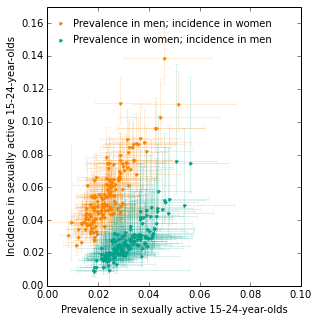
\includegraphics[width=7.5cm]{local_authorities_files/local_authorities_29_1.png}\end{center}
        \caption{Sampled incidence in each sex against prevalence in the other. Markers and error bars indicate median samples and central 95\% credible intervals. }
        \label{}
    \end{figure}
    
    Orange indicates the relationship between prevalence in men and
incidence in women, and green shows the relationship between prevalence
in women and incidence in men.

An natural question is why some LAs have higher incidence and prevalence
than others. One possibility is that higher screening rates in some
areas lower prevalence and incidence. To investigate this, we plot
incidence against screening in men and women:

    \begin{footnotesize}
        \begin{Verbatim}[commandchars=\\\{\}]
{\color{incolor}In [{\color{incolor}16}]:} \PY{c}{\PYZsh{} Figure 11}
         
         \PY{n}{fig} \PY{o}{=} \PY{n}{plt}\PY{o}{.}\PY{n}{figure}\PY{p}{(}\PY{n}{figsize} \PY{o}{=} \PY{p}{(}\PY{l+m+mi}{10}\PY{p}{,}\PY{l+m+mi}{10}\PY{p}{)}\PY{p}{)}
         \PY{n}{ax1} \PY{o}{=} \PY{n}{fig}\PY{o}{.}\PY{n}{add\PYZus{}subplot}\PY{p}{(}\PY{l+m+mi}{221}\PY{p}{)}
         \PY{n}{ax2} \PY{o}{=} \PY{n}{fig}\PY{o}{.}\PY{n}{add\PYZus{}subplot}\PY{p}{(}\PY{l+m+mi}{222}\PY{p}{)}
         \PY{n}{ax3} \PY{o}{=} \PY{n}{fig}\PY{o}{.}\PY{n}{add\PYZus{}subplot}\PY{p}{(}\PY{l+m+mi}{223}\PY{p}{)}
         \PY{n}{ax4} \PY{o}{=} \PY{n}{fig}\PY{o}{.}\PY{n}{add\PYZus{}subplot}\PY{p}{(}\PY{l+m+mi}{224}\PY{p}{)}
         
         \PY{n}{plt\PYZus{}ppc}\PY{p}{(}\PY{n}{ax1}\PY{p}{,} \PY{n}{scr\PYZus{}m\PYZus{}la}\PY{p}{,} \PY{n}{inc\PYZus{}m\PYZus{}la}\PY{p}{,} \PY{l+m+mi}{0}\PY{p}{,} \PY{l+m+mi}{95}\PY{p}{,} \PY{l+s}{\PYZsq{}}\PY{l+s}{b}\PY{l+s}{\PYZsq{}}\PY{p}{,} \PY{n}{alpha}\PY{o}{=}\PY{l+m+mf}{0.2}\PY{p}{)}
         \PY{n}{ax1}\PY{o}{.}\PY{n}{plot}\PY{p}{(}\PY{n}{percentile}\PY{p}{(}\PY{n}{scr\PYZus{}m\PYZus{}la}\PY{p}{,}\PY{l+m+mi}{50}\PY{p}{,}\PY{n}{axis}\PY{o}{=}\PY{l+m+mi}{0}\PY{p}{)}\PY{p}{,} \PY{n}{percentile}\PY{p}{(}\PY{n}{inc\PYZus{}m\PYZus{}la}\PY{p}{,}\PY{l+m+mi}{50}\PY{p}{,}\PY{n}{axis}\PY{o}{=}\PY{l+m+mi}{0}\PY{p}{)}\PY{p}{,} \PY{l+s}{\PYZsq{}}\PY{l+s}{.b}\PY{l+s}{\PYZsq{}}\PY{p}{)}
         \PY{n}{ax1}\PY{o}{.}\PY{n}{set\PYZus{}xlabel}\PY{p}{(}\PY{l+s}{\PYZsq{}}\PY{l+s}{Screening in men}\PY{l+s}{\PYZsq{}}\PY{p}{)}\PY{p}{;} \PY{n}{ax1}\PY{o}{.}\PY{n}{set\PYZus{}ylabel}\PY{p}{(}\PY{l+s}{\PYZsq{}}\PY{l+s}{Incidence in men}\PY{l+s}{\PYZsq{}}\PY{p}{)}
         
         \PY{n}{plt\PYZus{}ppc}\PY{p}{(}\PY{n}{ax2}\PY{p}{,} \PY{n}{scr\PYZus{}f\PYZus{}la}\PY{p}{,} \PY{n}{inc\PYZus{}m\PYZus{}la}\PY{p}{,} \PY{l+m+mi}{0}\PY{p}{,} \PY{l+m+mi}{95}\PY{p}{,} \PY{l+s}{\PYZsq{}}\PY{l+s}{\PYZsh{}00A08A}\PY{l+s}{\PYZsq{}}\PY{p}{,} \PY{n}{alpha}\PY{o}{=}\PY{l+m+mf}{0.2}\PY{p}{)}
         \PY{n}{ax2}\PY{o}{.}\PY{n}{plot}\PY{p}{(}\PY{n}{percentile}\PY{p}{(}\PY{n}{scr\PYZus{}f\PYZus{}la}\PY{p}{,}\PY{l+m+mi}{50}\PY{p}{,}\PY{n}{axis}\PY{o}{=}\PY{l+m+mi}{0}\PY{p}{)}\PY{p}{,} \PY{n}{percentile}\PY{p}{(}\PY{n}{inc\PYZus{}m\PYZus{}la}\PY{p}{,}\PY{l+m+mi}{50}\PY{p}{,}\PY{n}{axis}\PY{o}{=}\PY{l+m+mi}{0}\PY{p}{)}\PY{p}{,} \PY{l+s}{\PYZsq{}}\PY{l+s}{.}\PY{l+s}{\PYZsq{}}\PY{p}{,} \PY{n}{c}\PY{o}{=}\PY{l+s}{\PYZsq{}}\PY{l+s}{\PYZsh{}00A08A}\PY{l+s}{\PYZsq{}}\PY{p}{)}
         \PY{n}{ax2}\PY{o}{.}\PY{n}{set\PYZus{}xlabel}\PY{p}{(}\PY{l+s}{\PYZsq{}}\PY{l+s}{Screening in women}\PY{l+s}{\PYZsq{}}\PY{p}{)}\PY{p}{;} \PY{n}{ax2}\PY{o}{.}\PY{n}{set\PYZus{}ylabel}\PY{p}{(}\PY{l+s}{\PYZsq{}}\PY{l+s}{Incidence in men}\PY{l+s}{\PYZsq{}}\PY{p}{)}
         
         \PY{n}{plt\PYZus{}ppc}\PY{p}{(}\PY{n}{ax3}\PY{p}{,} \PY{n}{scr\PYZus{}m\PYZus{}la}\PY{p}{,} \PY{n}{inc\PYZus{}f\PYZus{}la}\PY{p}{,} \PY{l+m+mi}{0}\PY{p}{,} \PY{l+m+mi}{95}\PY{p}{,} \PY{l+s}{\PYZsq{}}\PY{l+s}{\PYZsh{}F98400}\PY{l+s}{\PYZsq{}}\PY{p}{,} \PY{n}{alpha}\PY{o}{=}\PY{l+m+mf}{0.2}\PY{p}{)}
         \PY{n}{ax3}\PY{o}{.}\PY{n}{plot}\PY{p}{(}\PY{n}{percentile}\PY{p}{(}\PY{n}{scr\PYZus{}m\PYZus{}la}\PY{p}{,}\PY{l+m+mi}{50}\PY{p}{,}\PY{n}{axis}\PY{o}{=}\PY{l+m+mi}{0}\PY{p}{)}\PY{p}{,} \PY{n}{percentile}\PY{p}{(}\PY{n}{inc\PYZus{}f\PYZus{}la}\PY{p}{,}\PY{l+m+mi}{50}\PY{p}{,}\PY{n}{axis}\PY{o}{=}\PY{l+m+mi}{0}\PY{p}{)}\PY{p}{,} \PY{l+s}{\PYZsq{}}\PY{l+s}{.}\PY{l+s}{\PYZsq{}}\PY{p}{,} \PY{n}{c}\PY{o}{=}\PY{l+s}{\PYZsq{}}\PY{l+s}{\PYZsh{}F98400}\PY{l+s}{\PYZsq{}}\PY{p}{)}
         \PY{n}{ax3}\PY{o}{.}\PY{n}{set\PYZus{}xlabel}\PY{p}{(}\PY{l+s}{\PYZsq{}}\PY{l+s}{Screening in men}\PY{l+s}{\PYZsq{}}\PY{p}{)}\PY{p}{;} \PY{n}{ax3}\PY{o}{.}\PY{n}{set\PYZus{}ylabel}\PY{p}{(}\PY{l+s}{\PYZsq{}}\PY{l+s}{Incidence in women}\PY{l+s}{\PYZsq{}}\PY{p}{)}
         
         \PY{n}{plt\PYZus{}ppc}\PY{p}{(}\PY{n}{ax4}\PY{p}{,} \PY{n}{scr\PYZus{}f\PYZus{}la}\PY{p}{,} \PY{n}{inc\PYZus{}f\PYZus{}la}\PY{p}{,} \PY{l+m+mi}{0}\PY{p}{,} \PY{l+m+mi}{95}\PY{p}{,} \PY{l+s}{\PYZsq{}}\PY{l+s}{r}\PY{l+s}{\PYZsq{}}\PY{p}{,} \PY{n}{alpha}\PY{o}{=}\PY{l+m+mf}{0.2}\PY{p}{)}
         \PY{n}{ax4}\PY{o}{.}\PY{n}{plot}\PY{p}{(}\PY{n}{percentile}\PY{p}{(}\PY{n}{scr\PYZus{}f\PYZus{}la}\PY{p}{,}\PY{l+m+mi}{50}\PY{p}{,}\PY{n}{axis}\PY{o}{=}\PY{l+m+mi}{0}\PY{p}{)}\PY{p}{,} \PY{n}{percentile}\PY{p}{(}\PY{n}{inc\PYZus{}f\PYZus{}la}\PY{p}{,}\PY{l+m+mi}{50}\PY{p}{,}\PY{n}{axis}\PY{o}{=}\PY{l+m+mi}{0}\PY{p}{)}\PY{p}{,} \PY{l+s}{\PYZsq{}}\PY{l+s}{.}\PY{l+s}{\PYZsq{}}\PY{p}{,} \PY{n}{c}\PY{o}{=}\PY{l+s}{\PYZsq{}}\PY{l+s}{r}\PY{l+s}{\PYZsq{}}\PY{p}{)}
         \PY{n}{ax4}\PY{o}{.}\PY{n}{set\PYZus{}xlabel}\PY{p}{(}\PY{l+s}{\PYZsq{}}\PY{l+s}{Screening in women}\PY{l+s}{\PYZsq{}}\PY{p}{)}\PY{p}{;} \PY{n}{ax4}\PY{o}{.}\PY{n}{set\PYZus{}ylabel}\PY{p}{(}\PY{l+s}{\PYZsq{}}\PY{l+s}{Incidence in women}\PY{l+s}{\PYZsq{}}\PY{p}{)}
\end{Verbatim}
    \end{footnotesize}

    \begin{footnotesize}
            \begin{Verbatim}[commandchars=\\\{\}]
{\color{outcolor}Out[{\color{outcolor}16}]:} <matplotlib.text.Text at 0x123d92bd0>
\end{Verbatim}
    \end{footnotesize}
        
    \begin{figure}
        \begin{center}\adjustimage{max size={0.9\linewidth}{0.4\paperheight}}{local_authorities_files/local_authorities_31_1.png}\end{center}
        \caption{Sampled incidence vs. screening rate. Markers and error bars indicate median samples and central 95\% credible intervals. Top-left: incidence in men vs. screening in men; top-right: incidence in men vs. screening in women; bottom-left: incidence in women vs. screening in men; bottom-right: incidence in women vs. screening in women.}
        \label{}
    \end{figure}
    
    \begin{footnotesize}
        \begin{Verbatim}[commandchars=\\\{\}]
{\color{incolor}In [{\color{incolor}17}]:} \PY{c}{\PYZsh{} Figure 12}
         
         \PY{c}{\PYZsh{} examine the Spearman correlation by sample}
         \PY{n}{spearman} \PY{o}{=} \PY{n}{empty}\PY{p}{(}\PY{p}{[}\PY{n}{n\PYZus{}sample}\PY{p}{,}\PY{l+m+mi}{4}\PY{p}{]}\PY{p}{)}
         
         \PY{k}{for} \PY{n}{i} \PY{o+ow}{in} \PY{n+nb}{xrange}\PY{p}{(}\PY{n}{shape}\PY{p}{(}\PY{n}{pos\PYZus{}m\PYZus{}la}\PY{p}{)}\PY{p}{[}\PY{l+m+mi}{0}\PY{p}{]}\PY{p}{)}\PY{p}{:}
             \PY{n}{spearman}\PY{p}{[}\PY{n}{i}\PY{p}{,}\PY{l+m+mi}{0}\PY{p}{]} \PY{o}{=} \PY{n}{stats}\PY{o}{.}\PY{n}{spearmanr}\PY{p}{(}\PY{n}{scr\PYZus{}m\PYZus{}la}\PY{p}{[}\PY{n}{i}\PY{p}{]}\PY{p}{,} \PY{n}{inc\PYZus{}m\PYZus{}la}\PY{p}{[}\PY{n}{i}\PY{p}{]}\PY{p}{)}\PY{p}{[}\PY{l+m+mi}{0}\PY{p}{]}
             \PY{n}{spearman}\PY{p}{[}\PY{n}{i}\PY{p}{,}\PY{l+m+mi}{1}\PY{p}{]} \PY{o}{=} \PY{n}{stats}\PY{o}{.}\PY{n}{spearmanr}\PY{p}{(}\PY{n}{scr\PYZus{}f\PYZus{}la}\PY{p}{[}\PY{n}{i}\PY{p}{]}\PY{p}{,} \PY{n}{inc\PYZus{}m\PYZus{}la}\PY{p}{[}\PY{n}{i}\PY{p}{]}\PY{p}{)}\PY{p}{[}\PY{l+m+mi}{0}\PY{p}{]}
             \PY{n}{spearman}\PY{p}{[}\PY{n}{i}\PY{p}{,}\PY{l+m+mi}{2}\PY{p}{]} \PY{o}{=} \PY{n}{stats}\PY{o}{.}\PY{n}{spearmanr}\PY{p}{(}\PY{n}{scr\PYZus{}m\PYZus{}la}\PY{p}{[}\PY{n}{i}\PY{p}{]}\PY{p}{,} \PY{n}{inc\PYZus{}f\PYZus{}la}\PY{p}{[}\PY{n}{i}\PY{p}{]}\PY{p}{)}\PY{p}{[}\PY{l+m+mi}{0}\PY{p}{]}
             \PY{n}{spearman}\PY{p}{[}\PY{n}{i}\PY{p}{,}\PY{l+m+mi}{3}\PY{p}{]} \PY{o}{=} \PY{n}{stats}\PY{o}{.}\PY{n}{spearmanr}\PY{p}{(}\PY{n}{scr\PYZus{}f\PYZus{}la}\PY{p}{[}\PY{n}{i}\PY{p}{]}\PY{p}{,} \PY{n}{inc\PYZus{}f\PYZus{}la}\PY{p}{[}\PY{n}{i}\PY{p}{]}\PY{p}{)}\PY{p}{[}\PY{l+m+mi}{0}\PY{p}{]}
         
         \PY{n}{mpl}\PY{o}{.}\PY{n}{rcParams}\PY{p}{[}\PY{l+s}{\PYZsq{}}\PY{l+s}{axes.color\PYZus{}cycle}\PY{l+s}{\PYZsq{}}\PY{p}{]} \PY{o}{=} \PY{p}{[}\PY{l+s}{\PYZsq{}}\PY{l+s}{b}\PY{l+s}{\PYZsq{}}\PY{p}{,}\PY{l+s}{\PYZsq{}}\PY{l+s}{\PYZsh{}00A08A}\PY{l+s}{\PYZsq{}}\PY{p}{,}\PY{l+s}{\PYZsq{}}\PY{l+s}{\PYZsh{}F98400}\PY{l+s}{\PYZsq{}}\PY{p}{,}\PY{l+s}{\PYZsq{}}\PY{l+s}{r}\PY{l+s}{\PYZsq{}}\PY{p}{]}
         \PY{n}{h}\PY{o}{=}\PY{n}{plt}\PY{o}{.}\PY{n}{hist}\PY{p}{(}\PY{n}{spearman}\PY{p}{,} \PY{l+m+mi}{20}\PY{p}{,} \PY{n}{histtype}\PY{o}{=}\PY{l+s}{\PYZsq{}}\PY{l+s}{step}\PY{l+s}{\PYZsq{}}\PY{p}{,} \PY{p}{)}
         \PY{n}{plt}\PY{o}{.}\PY{n}{xlabel}\PY{p}{(}\PY{l+s}{\PYZsq{}}\PY{l+s}{Spearman correlation coefficient}\PY{l+s}{\PYZsq{}}\PY{p}{)}
         \PY{n}{plt}\PY{o}{.}\PY{n}{ylabel}\PY{p}{(}\PY{l+s}{\PYZsq{}}\PY{l+s}{Frequency}\PY{l+s}{\PYZsq{}}\PY{p}{)}
\end{Verbatim}
    \end{footnotesize}

    \begin{footnotesize}
            \begin{Verbatim}[commandchars=\\\{\}]
{\color{outcolor}Out[{\color{outcolor}17}]:} <matplotlib.text.Text at 0x12415b110>
\end{Verbatim}
    \end{footnotesize}
        
    \begin{figure}
        \begin{center}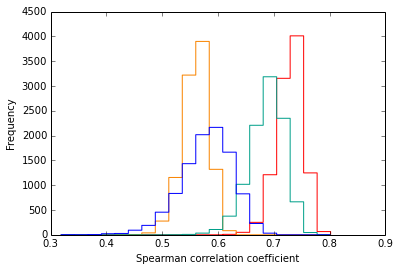
\includegraphics[width=10cm]{local_authorities_files/local_authorities_32_1.png}\end{center}
        \caption{Spearman correlations between screening and incidence, at each of 10000 samples. Blue: incidence in men vs. screening in men; green: incidence in men vs. screening in women; orange: incidence in women vs. screening in men; red: incidence in women vs. screening in women.}
        \label{}
    \end{figure}
    
    (Colours correspond to marker colours in the plot above.) In fact, the
positive correlations show that areas with more screening tend to have
higher incidence.

We also examine the relationship with prevalence:

    \begin{footnotesize}
        \begin{Verbatim}[commandchars=\\\{\}]
{\color{incolor}In [{\color{incolor}18}]:} \PY{c}{\PYZsh{} Figure 13}
         
         \PY{n}{fig} \PY{o}{=} \PY{n}{plt}\PY{o}{.}\PY{n}{figure}\PY{p}{(}\PY{n}{figsize} \PY{o}{=} \PY{p}{(}\PY{l+m+mi}{10}\PY{p}{,}\PY{l+m+mi}{10}\PY{p}{)}\PY{p}{)}
         \PY{n}{ax1} \PY{o}{=} \PY{n}{fig}\PY{o}{.}\PY{n}{add\PYZus{}subplot}\PY{p}{(}\PY{l+m+mi}{221}\PY{p}{)}
         \PY{n}{ax2} \PY{o}{=} \PY{n}{fig}\PY{o}{.}\PY{n}{add\PYZus{}subplot}\PY{p}{(}\PY{l+m+mi}{222}\PY{p}{)}
         \PY{n}{ax3} \PY{o}{=} \PY{n}{fig}\PY{o}{.}\PY{n}{add\PYZus{}subplot}\PY{p}{(}\PY{l+m+mi}{223}\PY{p}{)}
         \PY{n}{ax4} \PY{o}{=} \PY{n}{fig}\PY{o}{.}\PY{n}{add\PYZus{}subplot}\PY{p}{(}\PY{l+m+mi}{224}\PY{p}{)}
         
         \PY{n}{plt\PYZus{}ppc}\PY{p}{(}\PY{n}{ax1}\PY{p}{,} \PY{n}{scr\PYZus{}m\PYZus{}la}\PY{p}{,} \PY{n}{prev\PYZus{}m\PYZus{}la}\PY{p}{,} \PY{l+m+mi}{0}\PY{p}{,} \PY{l+m+mi}{95}\PY{p}{,} \PY{l+s}{\PYZsq{}}\PY{l+s}{b}\PY{l+s}{\PYZsq{}}\PY{p}{,} \PY{n}{alpha}\PY{o}{=}\PY{l+m+mf}{0.2}\PY{p}{)}
         \PY{n}{ax1}\PY{o}{.}\PY{n}{plot}\PY{p}{(}\PY{n}{percentile}\PY{p}{(}\PY{n}{scr\PYZus{}m\PYZus{}la}\PY{p}{,}\PY{l+m+mi}{50}\PY{p}{,}\PY{n}{axis}\PY{o}{=}\PY{l+m+mi}{0}\PY{p}{)}\PY{p}{,} \PY{n}{percentile}\PY{p}{(}\PY{n}{prev\PYZus{}m\PYZus{}la}\PY{p}{,}\PY{l+m+mi}{50}\PY{p}{,}\PY{n}{axis}\PY{o}{=}\PY{l+m+mi}{0}\PY{p}{)}\PY{p}{,} \PY{l+s}{\PYZsq{}}\PY{l+s}{.b}\PY{l+s}{\PYZsq{}}\PY{p}{)}
         \PY{n}{ax1}\PY{o}{.}\PY{n}{set\PYZus{}xlabel}\PY{p}{(}\PY{l+s}{\PYZsq{}}\PY{l+s}{Screening in men}\PY{l+s}{\PYZsq{}}\PY{p}{)}\PY{p}{;} \PY{n}{ax1}\PY{o}{.}\PY{n}{set\PYZus{}ylabel}\PY{p}{(}\PY{l+s}{\PYZsq{}}\PY{l+s}{Prevalence in men}\PY{l+s}{\PYZsq{}}\PY{p}{)}
         
         \PY{n}{plt\PYZus{}ppc}\PY{p}{(}\PY{n}{ax2}\PY{p}{,} \PY{n}{scr\PYZus{}f\PYZus{}la}\PY{p}{,} \PY{n}{prev\PYZus{}m\PYZus{}la}\PY{p}{,} \PY{l+m+mi}{0}\PY{p}{,} \PY{l+m+mi}{95}\PY{p}{,} \PY{l+s}{\PYZsq{}}\PY{l+s}{\PYZsh{}00A08A}\PY{l+s}{\PYZsq{}}\PY{p}{,} \PY{n}{alpha}\PY{o}{=}\PY{l+m+mf}{0.2}\PY{p}{)}
         \PY{n}{ax2}\PY{o}{.}\PY{n}{plot}\PY{p}{(}\PY{n}{percentile}\PY{p}{(}\PY{n}{scr\PYZus{}f\PYZus{}la}\PY{p}{,}\PY{l+m+mi}{50}\PY{p}{,}\PY{n}{axis}\PY{o}{=}\PY{l+m+mi}{0}\PY{p}{)}\PY{p}{,} \PY{n}{percentile}\PY{p}{(}\PY{n}{prev\PYZus{}m\PYZus{}la}\PY{p}{,}\PY{l+m+mi}{50}\PY{p}{,}\PY{n}{axis}\PY{o}{=}\PY{l+m+mi}{0}\PY{p}{)}\PY{p}{,} \PY{l+s}{\PYZsq{}}\PY{l+s}{.}\PY{l+s}{\PYZsq{}}\PY{p}{,} \PY{n}{c}\PY{o}{=}\PY{l+s}{\PYZsq{}}\PY{l+s}{\PYZsh{}00A08A}\PY{l+s}{\PYZsq{}}\PY{p}{)}
         \PY{n}{ax2}\PY{o}{.}\PY{n}{set\PYZus{}xlabel}\PY{p}{(}\PY{l+s}{\PYZsq{}}\PY{l+s}{Screening in women}\PY{l+s}{\PYZsq{}}\PY{p}{)}\PY{p}{;} \PY{n}{ax2}\PY{o}{.}\PY{n}{set\PYZus{}ylabel}\PY{p}{(}\PY{l+s}{\PYZsq{}}\PY{l+s}{Prevalence in men}\PY{l+s}{\PYZsq{}}\PY{p}{)}
         
         \PY{n}{plt\PYZus{}ppc}\PY{p}{(}\PY{n}{ax3}\PY{p}{,} \PY{n}{scr\PYZus{}m\PYZus{}la}\PY{p}{,} \PY{n}{prev\PYZus{}f\PYZus{}la}\PY{p}{,} \PY{l+m+mi}{0}\PY{p}{,} \PY{l+m+mi}{95}\PY{p}{,} \PY{l+s}{\PYZsq{}}\PY{l+s}{\PYZsh{}F98400}\PY{l+s}{\PYZsq{}}\PY{p}{,} \PY{n}{alpha}\PY{o}{=}\PY{l+m+mf}{0.2}\PY{p}{)}
         \PY{n}{ax3}\PY{o}{.}\PY{n}{plot}\PY{p}{(}\PY{n}{percentile}\PY{p}{(}\PY{n}{scr\PYZus{}m\PYZus{}la}\PY{p}{,}\PY{l+m+mi}{50}\PY{p}{,}\PY{n}{axis}\PY{o}{=}\PY{l+m+mi}{0}\PY{p}{)}\PY{p}{,} \PY{n}{percentile}\PY{p}{(}\PY{n}{prev\PYZus{}f\PYZus{}la}\PY{p}{,}\PY{l+m+mi}{50}\PY{p}{,}\PY{n}{axis}\PY{o}{=}\PY{l+m+mi}{0}\PY{p}{)}\PY{p}{,} \PY{l+s}{\PYZsq{}}\PY{l+s}{.}\PY{l+s}{\PYZsq{}}\PY{p}{,} \PY{n}{c}\PY{o}{=}\PY{l+s}{\PYZsq{}}\PY{l+s}{\PYZsh{}F98400}\PY{l+s}{\PYZsq{}}\PY{p}{)}
         \PY{n}{ax3}\PY{o}{.}\PY{n}{set\PYZus{}xlabel}\PY{p}{(}\PY{l+s}{\PYZsq{}}\PY{l+s}{Screening in men}\PY{l+s}{\PYZsq{}}\PY{p}{)}\PY{p}{;} \PY{n}{ax3}\PY{o}{.}\PY{n}{set\PYZus{}ylabel}\PY{p}{(}\PY{l+s}{\PYZsq{}}\PY{l+s}{Prevalence in women}\PY{l+s}{\PYZsq{}}\PY{p}{)}
         
         \PY{n}{plt\PYZus{}ppc}\PY{p}{(}\PY{n}{ax4}\PY{p}{,} \PY{n}{scr\PYZus{}f\PYZus{}la}\PY{p}{,} \PY{n}{prev\PYZus{}f\PYZus{}la}\PY{p}{,} \PY{l+m+mi}{0}\PY{p}{,} \PY{l+m+mi}{95}\PY{p}{,} \PY{l+s}{\PYZsq{}}\PY{l+s}{r}\PY{l+s}{\PYZsq{}}\PY{p}{,} \PY{n}{alpha}\PY{o}{=}\PY{l+m+mf}{0.2}\PY{p}{)}
         \PY{n}{ax4}\PY{o}{.}\PY{n}{plot}\PY{p}{(}\PY{n}{percentile}\PY{p}{(}\PY{n}{scr\PYZus{}f\PYZus{}la}\PY{p}{,}\PY{l+m+mi}{50}\PY{p}{,}\PY{n}{axis}\PY{o}{=}\PY{l+m+mi}{0}\PY{p}{)}\PY{p}{,} \PY{n}{percentile}\PY{p}{(}\PY{n}{prev\PYZus{}f\PYZus{}la}\PY{p}{,}\PY{l+m+mi}{50}\PY{p}{,}\PY{n}{axis}\PY{o}{=}\PY{l+m+mi}{0}\PY{p}{)}\PY{p}{,} \PY{l+s}{\PYZsq{}}\PY{l+s}{.}\PY{l+s}{\PYZsq{}}\PY{p}{,} \PY{n}{c}\PY{o}{=}\PY{l+s}{\PYZsq{}}\PY{l+s}{r}\PY{l+s}{\PYZsq{}}\PY{p}{)}
         \PY{n}{ax4}\PY{o}{.}\PY{n}{set\PYZus{}xlabel}\PY{p}{(}\PY{l+s}{\PYZsq{}}\PY{l+s}{Screening in women}\PY{l+s}{\PYZsq{}}\PY{p}{)}\PY{p}{;} \PY{n}{ax4}\PY{o}{.}\PY{n}{set\PYZus{}ylabel}\PY{p}{(}\PY{l+s}{\PYZsq{}}\PY{l+s}{Prevalence in women}\PY{l+s}{\PYZsq{}}\PY{p}{)}
\end{Verbatim}
    \end{footnotesize}

    \begin{footnotesize}
            \begin{Verbatim}[commandchars=\\\{\}]
{\color{outcolor}Out[{\color{outcolor}18}]:} <matplotlib.text.Text at 0x1245c8c90>
\end{Verbatim}
    \end{footnotesize}
        
    \begin{figure}
        \begin{center}\adjustimage{max size={0.9\linewidth}{0.4\paperheight}}{local_authorities_files/local_authorities_34_1.png}\end{center}
        \caption{Sampled prevalence vs. screening rate. Markers and error bars indicate median samples and central 95\% credible intervals. Top-left: prevalence in men vs. screening in men; top-right: prevalence in men vs. screening in women; bottom-left: prevalence in women vs. screening in men; bottom-right: prevalence in women vs. screening in women.}
        \label{}
    \end{figure}
    
    \begin{footnotesize}
        \begin{Verbatim}[commandchars=\\\{\}]
{\color{incolor}In [{\color{incolor}19}]:} \PY{c}{\PYZsh{} Figure 14}
         \PY{c}{\PYZsh{} examine the Spearman correlation by sample}
         \PY{n}{spearman} \PY{o}{=} \PY{n}{empty}\PY{p}{(}\PY{p}{[}\PY{n}{n\PYZus{}sample}\PY{p}{,}\PY{l+m+mi}{4}\PY{p}{]}\PY{p}{)}
         
         \PY{k}{for} \PY{n}{i} \PY{o+ow}{in} \PY{n+nb}{xrange}\PY{p}{(}\PY{n}{shape}\PY{p}{(}\PY{n}{pos\PYZus{}m\PYZus{}la}\PY{p}{)}\PY{p}{[}\PY{l+m+mi}{0}\PY{p}{]}\PY{p}{)}\PY{p}{:}
             \PY{n}{spearman}\PY{p}{[}\PY{n}{i}\PY{p}{,}\PY{l+m+mi}{0}\PY{p}{]} \PY{o}{=} \PY{n}{stats}\PY{o}{.}\PY{n}{spearmanr}\PY{p}{(}\PY{n}{scr\PYZus{}m\PYZus{}la}\PY{p}{[}\PY{n}{i}\PY{p}{]}\PY{p}{,} \PY{n}{prev\PYZus{}m\PYZus{}la}\PY{p}{[}\PY{n}{i}\PY{p}{]}\PY{p}{)}\PY{p}{[}\PY{l+m+mi}{0}\PY{p}{]}
             \PY{n}{spearman}\PY{p}{[}\PY{n}{i}\PY{p}{,}\PY{l+m+mi}{1}\PY{p}{]} \PY{o}{=} \PY{n}{stats}\PY{o}{.}\PY{n}{spearmanr}\PY{p}{(}\PY{n}{scr\PYZus{}f\PYZus{}la}\PY{p}{[}\PY{n}{i}\PY{p}{]}\PY{p}{,} \PY{n}{prev\PYZus{}m\PYZus{}la}\PY{p}{[}\PY{n}{i}\PY{p}{]}\PY{p}{)}\PY{p}{[}\PY{l+m+mi}{0}\PY{p}{]}
             \PY{n}{spearman}\PY{p}{[}\PY{n}{i}\PY{p}{,}\PY{l+m+mi}{2}\PY{p}{]} \PY{o}{=} \PY{n}{stats}\PY{o}{.}\PY{n}{spearmanr}\PY{p}{(}\PY{n}{scr\PYZus{}m\PYZus{}la}\PY{p}{[}\PY{n}{i}\PY{p}{]}\PY{p}{,} \PY{n}{prev\PYZus{}f\PYZus{}la}\PY{p}{[}\PY{n}{i}\PY{p}{]}\PY{p}{)}\PY{p}{[}\PY{l+m+mi}{0}\PY{p}{]}
             \PY{n}{spearman}\PY{p}{[}\PY{n}{i}\PY{p}{,}\PY{l+m+mi}{3}\PY{p}{]} \PY{o}{=} \PY{n}{stats}\PY{o}{.}\PY{n}{spearmanr}\PY{p}{(}\PY{n}{scr\PYZus{}f\PYZus{}la}\PY{p}{[}\PY{n}{i}\PY{p}{]}\PY{p}{,} \PY{n}{prev\PYZus{}f\PYZus{}la}\PY{p}{[}\PY{n}{i}\PY{p}{]}\PY{p}{)}\PY{p}{[}\PY{l+m+mi}{0}\PY{p}{]}
             
         \PY{n}{h}\PY{o}{=}\PY{n}{plt}\PY{o}{.}\PY{n}{hist}\PY{p}{(}\PY{n}{spearman}\PY{p}{,} \PY{l+m+mi}{20}\PY{p}{,} \PY{n}{histtype}\PY{o}{=}\PY{l+s}{\PYZsq{}}\PY{l+s}{step}\PY{l+s}{\PYZsq{}}\PY{p}{,} \PY{p}{)}
         \PY{n}{plt}\PY{o}{.}\PY{n}{xlabel}\PY{p}{(}\PY{l+s}{\PYZsq{}}\PY{l+s}{Spearman correlation coefficient}\PY{l+s}{\PYZsq{}}\PY{p}{)}
         \PY{n}{plt}\PY{o}{.}\PY{n}{ylabel}\PY{p}{(}\PY{l+s}{\PYZsq{}}\PY{l+s}{Frequency}\PY{l+s}{\PYZsq{}}\PY{p}{)}
\end{Verbatim}
    \end{footnotesize}

    \begin{footnotesize}
            \begin{Verbatim}[commandchars=\\\{\}]
{\color{outcolor}Out[{\color{outcolor}19}]:} <matplotlib.text.Text at 0x1247e59d0>
\end{Verbatim}
    \end{footnotesize}
        
    \begin{figure}
        \begin{center}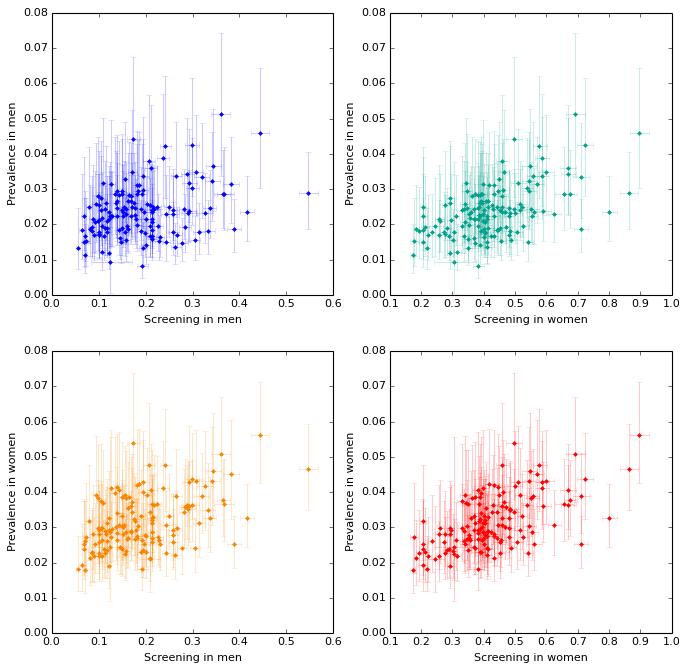
\includegraphics[width=10cm]{local_authorities_files/local_authorities_35_1.png}\end{center}
        \caption{Spearman correlations between screening and prevalence, at each of 10000 samples. Blue: prevalence in men vs. screening in men; green: prevalence in men vs. screening in women; orange: prevalence in women vs. screening in men; red: prevalence in women vs. screening in women.}
        \label{}
    \end{figure}
    
    Prevalence is also generally higher in areas with more screening.

What about the relationship between screening in men vs.~women, and
screening in men vs.~women?

    \begin{footnotesize}
        \begin{Verbatim}[commandchars=\\\{\}]
{\color{incolor}In [{\color{incolor}20}]:} \PY{c}{\PYZsh{} Figure 15}
         
         \PY{n}{fig} \PY{o}{=} \PY{n}{plt}\PY{o}{.}\PY{n}{figure}\PY{p}{(}\PY{n}{figsize} \PY{o}{=} \PY{p}{(}\PY{l+m+mi}{10}\PY{p}{,}\PY{l+m+mi}{5}\PY{p}{)}\PY{p}{)}
         
         \PY{n}{ax1} \PY{o}{=} \PY{n}{fig}\PY{o}{.}\PY{n}{add\PYZus{}subplot}\PY{p}{(}\PY{l+m+mi}{121}\PY{p}{)}
         \PY{n}{plt\PYZus{}ppc}\PY{p}{(}\PY{n}{ax1}\PY{p}{,} \PY{n}{prev\PYZus{}m\PYZus{}la}\PY{p}{,} \PY{n}{prev\PYZus{}f\PYZus{}la}\PY{p}{,} \PY{l+m+mi}{0}\PY{p}{,} \PY{l+m+mi}{95}\PY{p}{,} \PY{l+s}{\PYZsq{}}\PY{l+s}{k}\PY{l+s}{\PYZsq{}}\PY{p}{,} \PY{n}{alpha}\PY{o}{=}\PY{l+m+mf}{0.15}\PY{p}{)}
         \PY{n}{p} \PY{o}{=} \PY{n}{ax1}\PY{o}{.}\PY{n}{plot}\PY{p}{(}\PY{n}{percentile}\PY{p}{(}\PY{n}{prev\PYZus{}m\PYZus{}la}\PY{p}{,}\PY{l+m+mi}{50}\PY{p}{,}\PY{l+m+mi}{0}\PY{p}{)}\PY{p}{,} \PY{n}{percentile}\PY{p}{(}\PY{n}{prev\PYZus{}f\PYZus{}la}\PY{p}{,}\PY{l+m+mi}{50}\PY{p}{,}\PY{l+m+mi}{0}\PY{p}{)}\PY{p}{,} \PY{l+s}{\PYZsq{}}\PY{l+s}{.}\PY{l+s}{\PYZsq{}}\PY{p}{,} \PY{n}{color}\PY{o}{=}\PY{l+s}{\PYZsq{}}\PY{l+s}{k}\PY{l+s}{\PYZsq{}}\PY{p}{)}
         \PY{n}{ax1}\PY{o}{.}\PY{n}{set\PYZus{}xlim}\PY{p}{(}\PY{l+m+mi}{0}\PY{p}{,}\PY{l+m+mf}{0.1}\PY{p}{)}
         \PY{n}{ax1}\PY{o}{.}\PY{n}{set\PYZus{}ylim}\PY{p}{(}\PY{l+m+mi}{0}\PY{p}{,}\PY{l+m+mf}{0.1}\PY{p}{)}
         \PY{n}{ax1}\PY{o}{.}\PY{n}{set\PYZus{}xlabel}\PY{p}{(}\PY{l+s}{\PYZsq{}}\PY{l+s}{Prevalence in men}\PY{l+s}{\PYZsq{}}\PY{p}{)}
         \PY{n}{ax1}\PY{o}{.}\PY{n}{set\PYZus{}ylabel}\PY{p}{(}\PY{l+s}{\PYZsq{}}\PY{l+s}{Prevalence in women}\PY{l+s}{\PYZsq{}}\PY{p}{)}
         
         \PY{n}{ax2} \PY{o}{=} \PY{n}{fig}\PY{o}{.}\PY{n}{add\PYZus{}subplot}\PY{p}{(}\PY{l+m+mi}{122}\PY{p}{)}
         \PY{n}{plt\PYZus{}ppc}\PY{p}{(}\PY{n}{ax2}\PY{p}{,} \PY{n}{scr\PYZus{}m\PYZus{}la}\PY{p}{,} \PY{n}{scr\PYZus{}f\PYZus{}la}\PY{p}{,} \PY{l+m+mi}{0}\PY{p}{,} \PY{l+m+mi}{95}\PY{p}{,} \PY{l+s}{\PYZsq{}}\PY{l+s}{k}\PY{l+s}{\PYZsq{}}\PY{p}{,} \PY{n}{alpha}\PY{o}{=}\PY{l+m+mf}{0.3}\PY{p}{)}
         \PY{n}{p} \PY{o}{=} \PY{n}{ax2}\PY{o}{.}\PY{n}{plot}\PY{p}{(}\PY{n}{percentile}\PY{p}{(}\PY{n}{scr\PYZus{}m\PYZus{}la}\PY{p}{,}\PY{l+m+mi}{50}\PY{p}{,}\PY{l+m+mi}{0}\PY{p}{)}\PY{p}{,} \PY{n}{percentile}\PY{p}{(}\PY{n}{scr\PYZus{}f\PYZus{}la}\PY{p}{,}\PY{l+m+mi}{50}\PY{p}{,}\PY{l+m+mi}{0}\PY{p}{)}\PY{p}{,} \PY{l+s}{\PYZsq{}}\PY{l+s}{.}\PY{l+s}{\PYZsq{}}\PY{p}{,} \PY{n}{color}\PY{o}{=}\PY{l+s}{\PYZsq{}}\PY{l+s}{k}\PY{l+s}{\PYZsq{}}\PY{p}{)}
         \PY{n}{ax2}\PY{o}{.}\PY{n}{set\PYZus{}xlim}\PY{p}{(}\PY{l+m+mi}{0}\PY{p}{,}\PY{l+m+mi}{1}\PY{p}{)}
         \PY{n}{ax2}\PY{o}{.}\PY{n}{set\PYZus{}ylim}\PY{p}{(}\PY{l+m+mi}{0}\PY{p}{,}\PY{l+m+mi}{1}\PY{p}{)}
         \PY{n}{ax2}\PY{o}{.}\PY{n}{set\PYZus{}xlabel}\PY{p}{(}\PY{l+s}{\PYZsq{}}\PY{l+s}{Screening in men}\PY{l+s}{\PYZsq{}}\PY{p}{)}
         \PY{n}{ax2}\PY{o}{.}\PY{n}{set\PYZus{}ylabel}\PY{p}{(}\PY{l+s}{\PYZsq{}}\PY{l+s}{Screening in women}\PY{l+s}{\PYZsq{}}\PY{p}{)}
\end{Verbatim}
    \end{footnotesize}

    \begin{footnotesize}
            \begin{Verbatim}[commandchars=\\\{\}]
{\color{outcolor}Out[{\color{outcolor}20}]:} <matplotlib.text.Text at 0x124c06890>
\end{Verbatim}
    \end{footnotesize}
        
    \begin{figure}
        \begin{center}\adjustimage{max size={0.9\linewidth}{0.4\paperheight}}{local_authorities_files/local_authorities_37_1.png}\end{center}
        \caption{Correlation in local prevalence (left) and screening (right) in men vs. women. Markers and error bars indicate median samples and central 95\% credible intervals.}
        \label{}
    \end{figure}
    
    Prevalence in men and women is positively correlated, because of the
incidence-prevalence relationship illustrated above. LAs with more
asymptomatic screening of men also tend to have more screening of women,
but all LAs have more screening in women than men.


    % Add a bibliography block to the postdoc
    
    
    
    \end{document}
